\section{Shock-tubes}

In this section, we focus on simulation of soot formation in shock-tubes using the constant volume reactor of omnisoot, and compare species mole fraction and soot yield and morphology (if available) with benchmark measurements. Figure~\ref{fig:shocktubeschem} (left pane) illustrates the schematics of a shock-tube along with the idealized wave diagram. Shock-tubes are typically designed as a several meter long cylindrical tube separated by thin diaphragm into a smaller driver section filled a high pressure inert gas, and a longer driven section with diluted reactants. When the diaphragm is ruptured, the first shock wave propagates through the reactant mixture. The front shock compresses the reactants adiabatically raising the temperature and pressure throughout the shock-tube from $\mathrm{T_1}$, $\mathrm{P_1}$ to $\mathrm{T_2}$, $\mathrm{P_2}$. The passage of the reflected shock from the end wall heats up the reactants for the second time reaching $\mathrm{T_5}$, $\mathrm{P_5}$. Figure~\ref{fig:shocktubeschem} (right pane) shows the first and second jump in pressure due to the front and reflected shocks, respectively, and the variation in soot volume fraction during the pyrolysis of 0.03\% benzene in Ar. The reflected shock creates a nearly still mixture with a constant temperature and pressure (as shown in left pane of Figure~\ref{fig:shocktubeschem}) which provides an ideal condition for kinetic studies and rate constant investigations~\citep{kee2017chemically}. Therefore, the use of a shock tube provides a unique opportunity for investigating the kinetics of soot formation from fuels and at various temperatures, pressures and concentrations.

However, the processes investigated in shock tubes are limited to short residence times usually 1-3 ms, so they can only be used to study early stages of soot formation such as inception and surface growth, and not for processes occurring at longer residence times such as coagulation and carbonization. Note that the residence time is calculated after the passage of reflected shock. There is a delay in the increase of volume fraction known as induction time, $\mathrm{\tau_{ind}}$. There has been a lot of research in the literature focused on induction time (similarly on ignition delay time) in shock tubes~\citep{fussey1978shock}, but it is not the focus of this work. Instead, here we mainly investigate the species concentrations and soot characteristics during the pyrolysis of hydrocarbons, especially methane, at atmospheric and higher pressure which can be used for the design and optimization of carbon black in plasma reactors~\citep{fulcheri2023energy}. 

\subsection{Methane pyrolysis data of \citet{agafonov2016unified}}

First, the pyrolysis of 5\% and 10\% $\mathrm{CH_4}$ diluted with Ar is investigated for the post-shock temperature range of 1800-3000 K and the pressure range of 4.7-7.1 bar. We assume the pressure linearly increase by temperature across the simulation cases. The obtained soot yields by were compared with the soot yield measured by \citet{agafonov2016unified} using a dual-beam absorption–emission technique. \citet{agafonov2016unified} reported yield$\times$E(m) at $\mathrm{\lambda}$=632~nm, and yield data was retrieved using E(m)=0.37 suggested therein. 




% run the shock-tube with other mechanisms and include the results in the Appendix

\begin{figure}[!htbp]
	\centering
	\begin{subfigure}[t]{0.4\textwidth}
		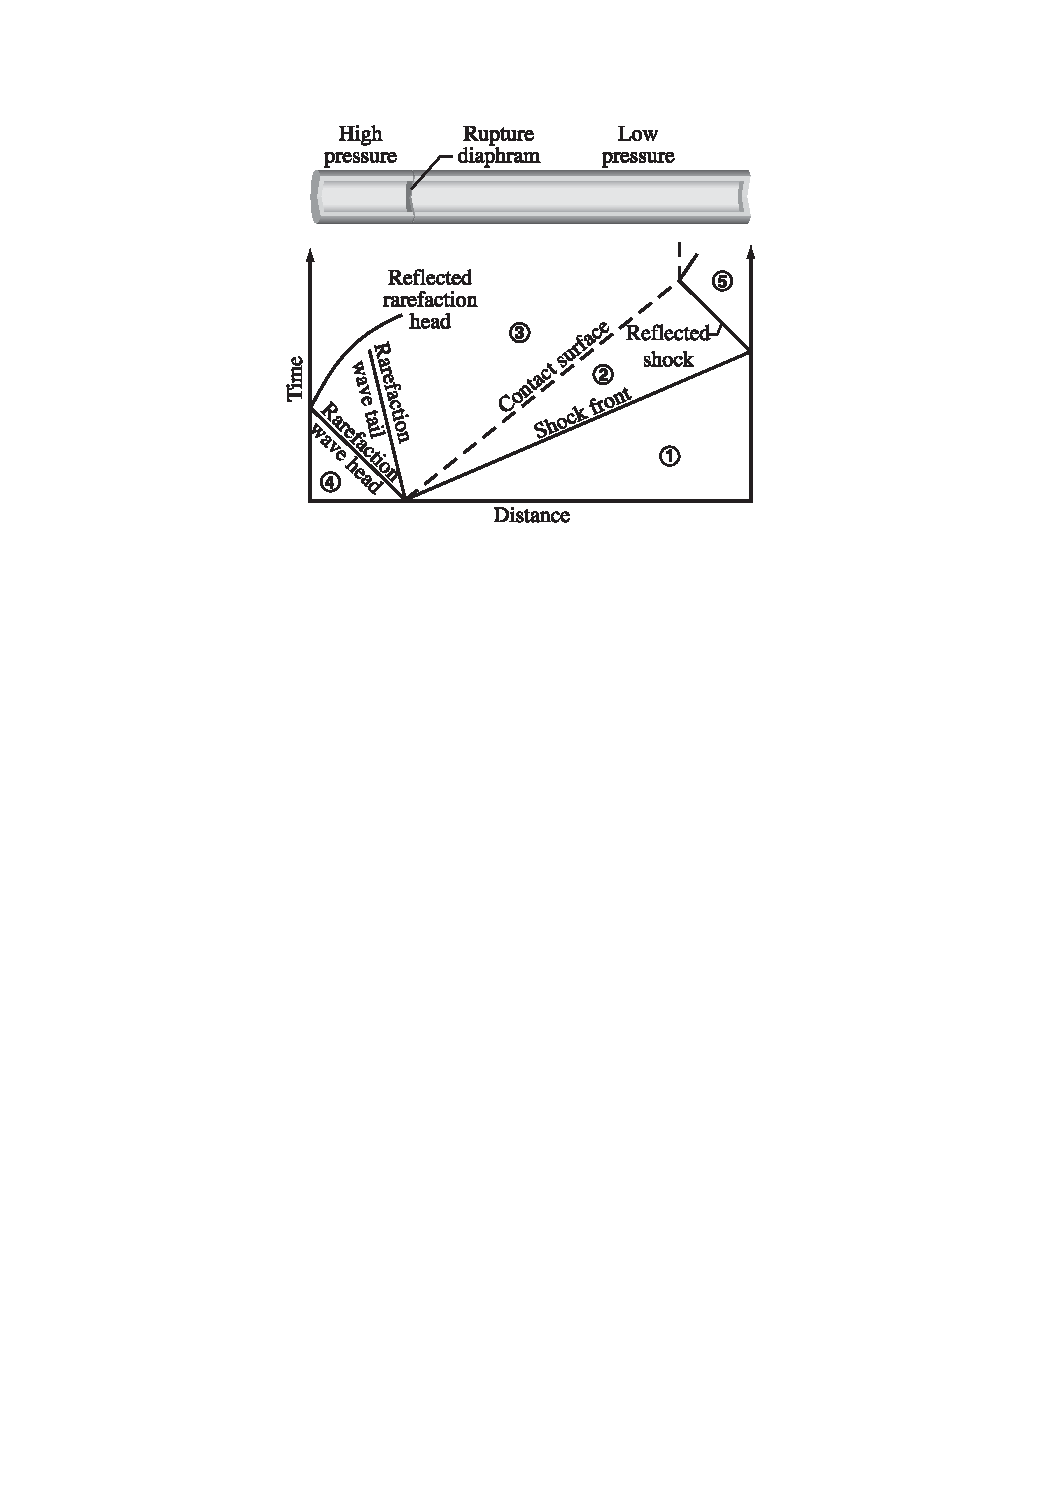
\includegraphics[width=1\textwidth]{Figures/Results/Shocktube/schematics.pdf}
	\end{subfigure}
	\begin{subfigure}[t]{0.4\textwidth}
	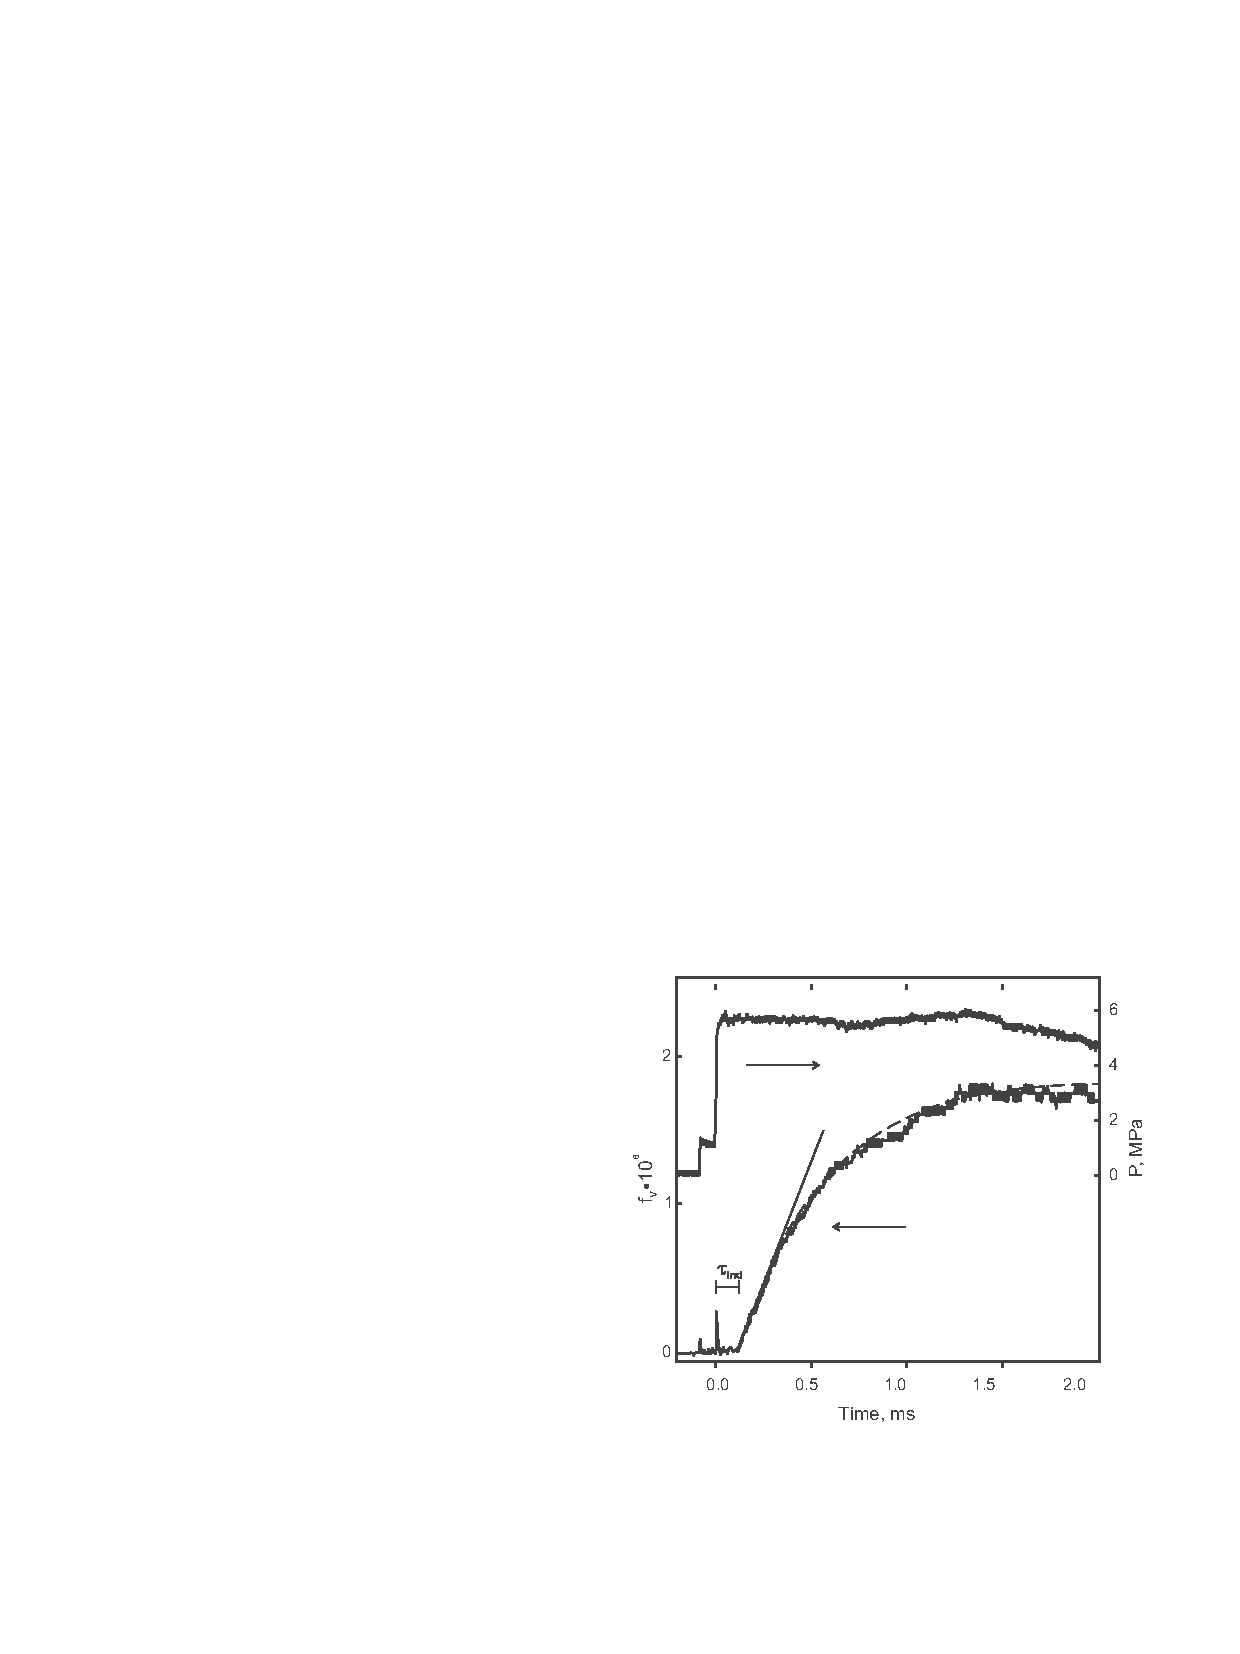
\includegraphics[width=1\textwidth]{Figures/Results/Shocktube/pfv_sample_shocktube.pdf}
	\end{subfigure}
	\caption{The schematics of a shock-tube and the idealized shockwave diagram(left pane reprinted from ~\citet{kee2017chemically}) and the variation of soot volume fraction measured by the extinction record at 633 nm and the pressure profile behind the reflected shock wave in a mixture 0.03\% benzene in Ar at T = 1890 K(right pane reprinted from ~\citet{karasevich1994soot})}
	\label{fig:shocktubeschem}
\end{figure}

Figure~\ref{fig:shocktubeyield} depicts soot yield (SY) at t=1.5 ms for 5\% and 10\% $\mathrm{CH_4}$ over the temperature range of 1800-3000 K using MPBM and SPBM and different inception model and Caltech~\citep{blanquart2009chemical} mechanism. Note that, the simulations were also performed using ABF~\citep{appel2000kinetic} and KAUST~\cite{wang2013pah} mechanisms, and the results were included in Appendix\hl{****}. The soot yield predictions exhibit a close agreement with measurements~\citep{agafonov2016unified} considering the uncertainties in residence time from experiments. The model also successfully captures the bell-shape dependence of soot yield on temperature that has been observed in a variety of hydrocarbons in shock tube~\citep{kellerer1996soot,knorre1996soot}. The particle dynamics model has minimal effect on the predicted soot yield. In the vicinity of peak soot yield, SPBM results in slightly lower yield than MPBM, but they are indistinguishable in the rest of the temperature range. 

%The minor difference between MPBM and SPBM is due to the short residence time (t=1.5 ms) where inception and surface growth are dominant leading to low polydispersity and relatively small agglomerates. 
In \%5 $\mathrm{CH_4}$, the SY peak temperature obtained from the model is slightly shifted towards higher temperatures (2300 K$<T_{peak}<$2400 K) compared to the measurements $T_{peak}=$2200 K. There are noticeable differences in the behavior of PAH growth model depending on the shock-tube initial temperature. When T$<$2100 K, Reactive Dimerization and EBridge Formation have the highest and lowest soot yield, respectively with Dimer Coalescence predicting soot yields that always falls between Reactive and Irreversible Dimerization. However, The soot yield of EBridge Formation rapidly rises with temperature and exceeds that of Reactive Dimerization and stays higher for the rest of temperature range.

The SY noticeably increases for higher initial $\mathrm{CH_4}$ mole fraction of \%10 because more PAH and $\mathrm{C_2H_2}$ are formed leading to stronger carbon conversion rate to soot via inception and surface growth. The peak SY obtained from the model occurs in a higher temperature range 2600-2700 K compared to \%5 $\mathrm{CH_4}$. Soot yield trends can be better understood by examining carbon mass fraction of species directly contributing to soot mass. Figure~\ref{fig:shocktubeAAAA} depicts the bell-shape distribution of the carbon mass fraction of soot precursors (A2, A2R5, A3, and A4) over the studied temperature range. In low (T=1800 K) and high (T=2300 K) end of distribution, a low amount of precursors are formed resulting in low inception rates, particle number concentration and surface growth sites that reduces the soot yield. Additionally, \%10$\mathrm{CH_4}$ has a wider spread with peaks at higher temperature compared to \%10$\mathrm{CH_4}$ which explains the shift in peak yield temperature in Figure~\ref{fig:shocktubeyield}. The effect of particle dynamics model is only noticeable in Reactive Dimerization where SPBM results in higher precursor CMF (lower consumption) due to its lower PAH adsorption rates. %Should discuss why the difference only appears in RD not the others


\begin{figure}[H]
	\centering
	\begin{subfigure}[t]{0.4\textwidth}
		\begin{tikzpicture}
			\draw (0, 0) node[inner sep=0] 	{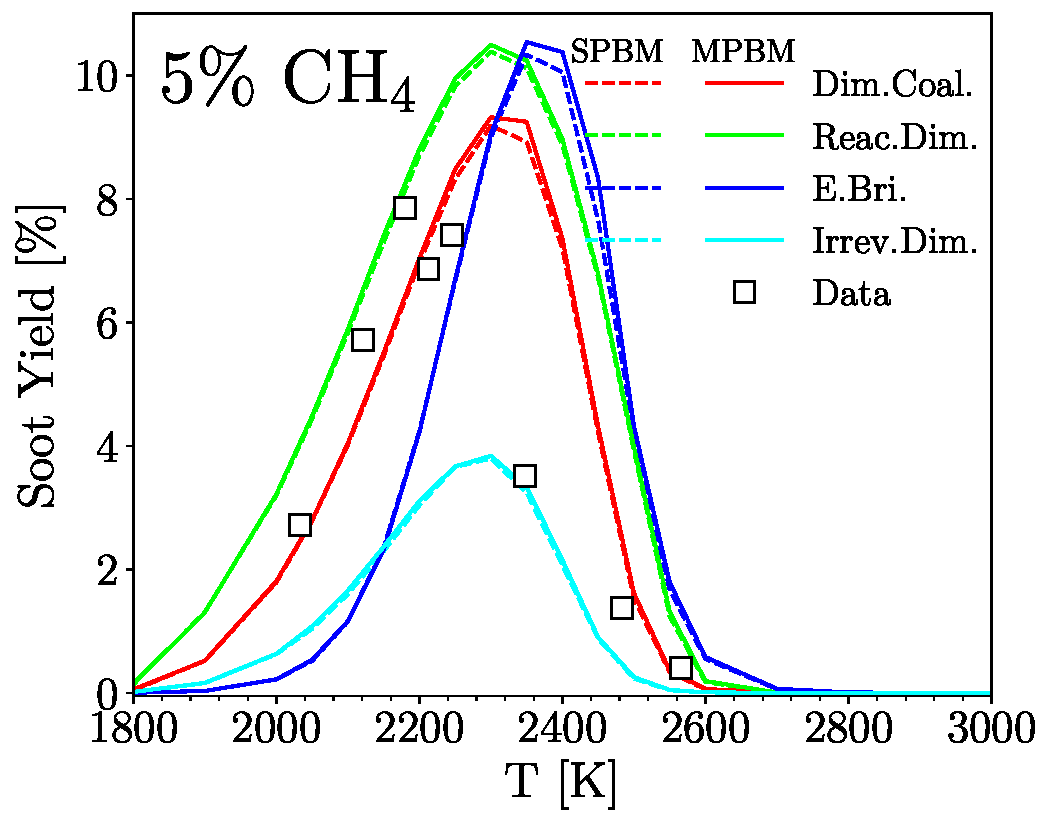
\includegraphics[width=1\textwidth]{Figures/Results/Shocktube/Agafonov2016/5CH4/carbon_yield.pdf}};
			\draw (2.44, 0.68) node {\tiny{\cite{agafonov2016unified}}};
		\end{tikzpicture}
	\end{subfigure}
	\begin{subfigure}[t]{0.4\textwidth}
	\begin{tikzpicture}
		\draw (0, 0) node[inner sep=0] 	{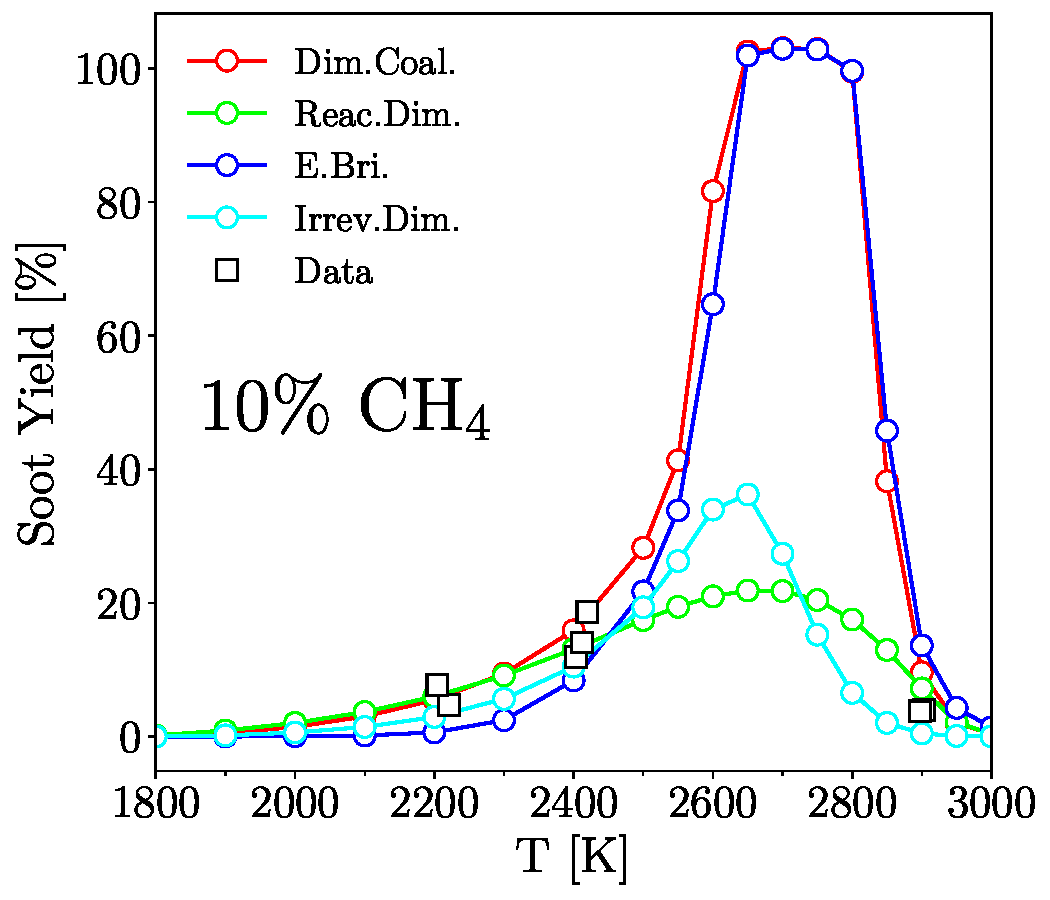
\includegraphics[width=1\textwidth]{Figures/Results/Shocktube/Agafonov2016/10CH4/carbon_yield.pdf}};
		\draw (0.29, -0.33) node {\tiny{\cite{agafonov2016unified}}};
	\end{tikzpicture}
	\end{subfigure}
	\caption{The temperature dependence of soot yield during pyrolysis of 5\%~$\mathrm{CH_4}$-Ar (left pane) and 10\%~$\mathrm{CH_4}$-Ar (right pane) at $\mathrm{P}$ = 4.5–6.7 bar obtained using Caltech mechanism and different inception models compared with measurements at 1.5ms~\cite{agafonov2016unified} where the absorption funtion of E(m)=0.37 is used to estimate soot yield.}
	\label{fig:shocktubeyield} 
\end{figure}


\begin{figure}[H]
	\centering
	\begin{subfigure}[t]{0.4\textwidth}
		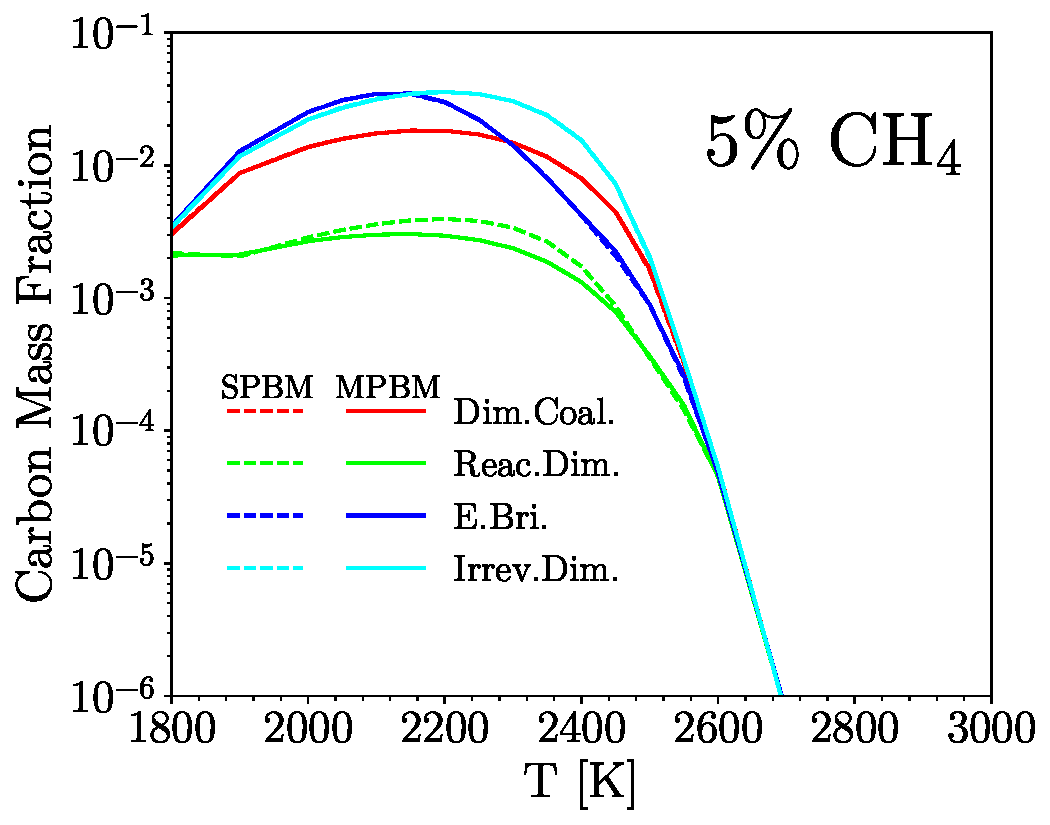
\includegraphics[width=1\textwidth]{Figures/Results/Shocktube/Agafonov2016/5CH4/AAAA.pdf}
	\end{subfigure}
	\begin{subfigure}[t]{0.4\textwidth}
		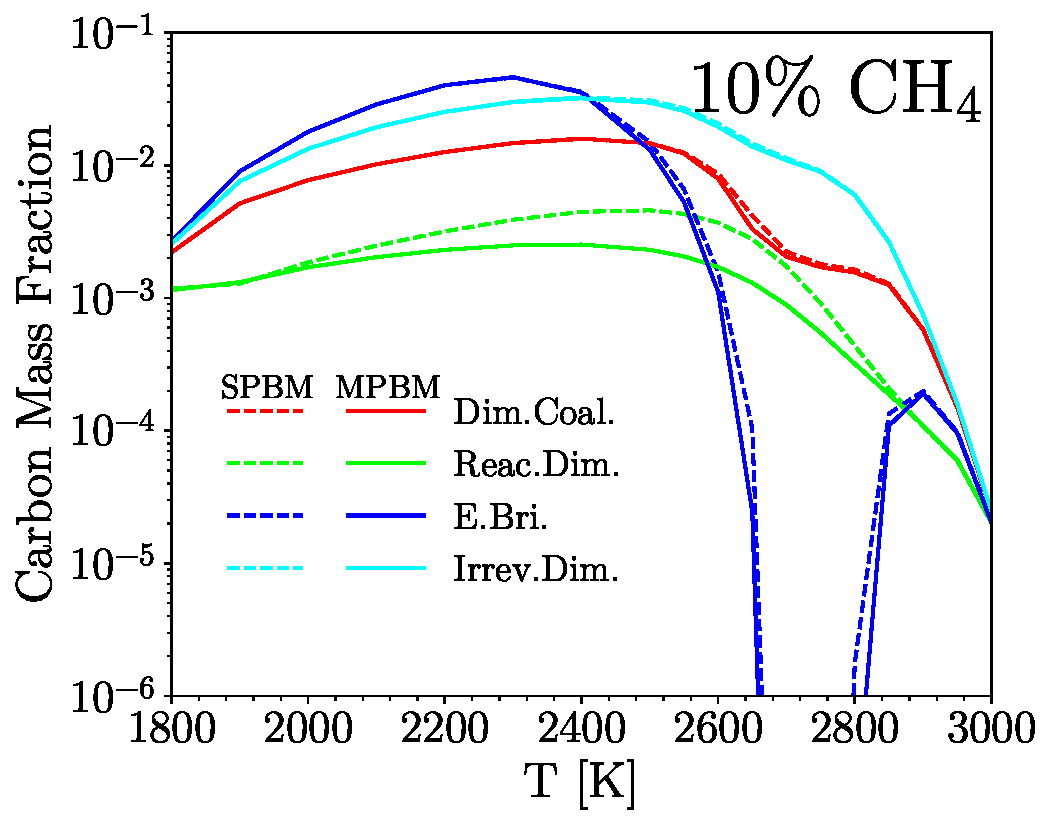
\includegraphics[width=1\textwidth]{Figures/Results/Shocktube/Agafonov2016/10CH4/AAAA.pdf}
	\end{subfigure}
	\caption{The temperature dependence of carbon mass fraction of soot precursors (A2, A2R5, A3, and A4) combined during pyrolysis of 5\%~$\mathrm{CH_4}$-Ar (left pane) and 10\%~$\mathrm{CH_4}$-Ar (right pane) at $\mathrm{P}$ = 4.5–6.7 bar obtained using Caltech mechanism and different inception models at t=1.5 ms}
	\label{fig:shocktubeAAAA} 
\end{figure}

EBridge Formation exhibits a similar behavior in \%10 $\mathrm{CH_4}$ simulations where it starts with the lowest SY at T$<$2500 K and then quickly increases reaching its peak at 100\% which is significantly larger that other PAH growth models. The remarkable drop in carbon mass fraction of precursors with EBridge Formation corresponds to \%100 yield meaning that all gaseous carbon including the precursors are directed towards soot particles.The higher precursor CMF with Irreversible Dimerization near the peak yield temperature region (2200-2400 K for \%5 $\mathrm{CH_4}$ and 2600-2800 K for \%10 $\mathrm{CH_4}$) indicates less consumption of precursors via inception and PAH adsorption.

Figure~\ref{fig:shocktubeC2H2} shows the CMF of $\mathrm{C_2H_2}$ that has an overall increasing trend in the temperature range, but it reaches a plateau for \%5 $\mathrm{CH_4}$. There is also a remarkable drop in $\mathrm{C_2H_2}$ CMF in 2600-2800 K due to strong mass growth rate of soot particles that drains $\mathrm{C_2H_2}$ from the gas mixture leading to high soot yield $\approxeq 100\%$. 


\begin{figure}[!htbp]
	\centering
	\begin{subfigure}[t]{0.4\textwidth}
		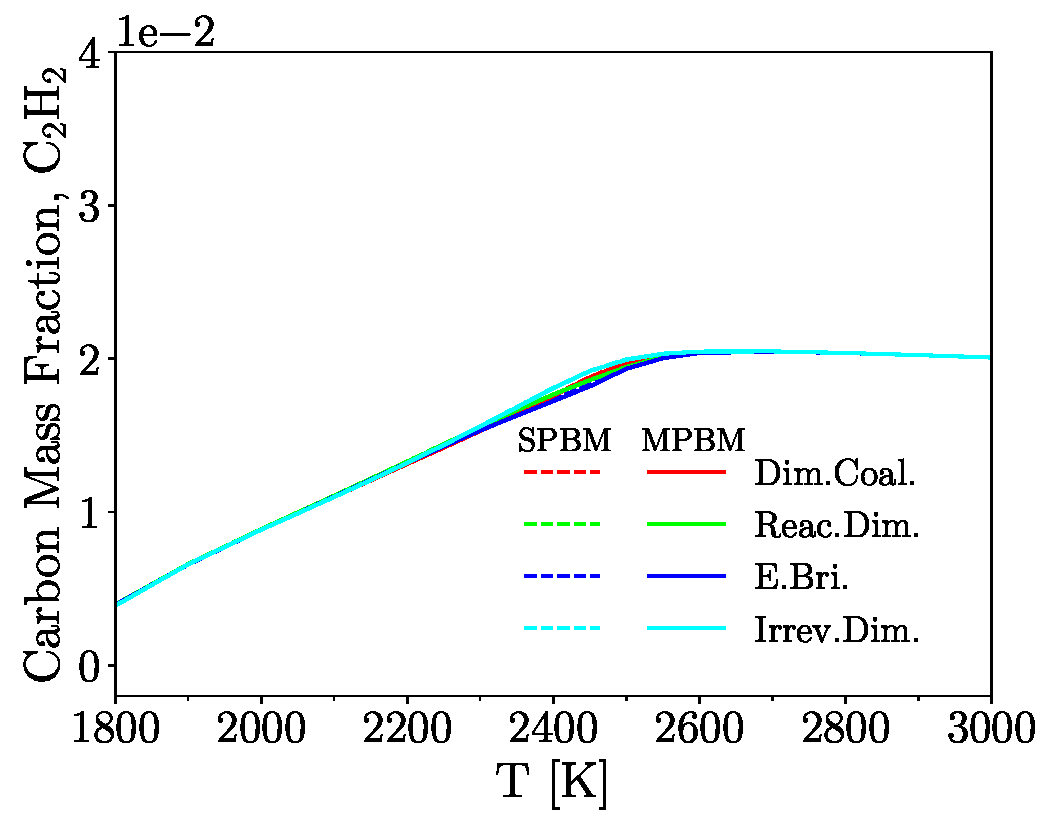
\includegraphics[width=1\textwidth]{Figures/Results/Shocktube/Agafonov2016/5CH4/C2H2.pdf}
	\end{subfigure}
	\begin{subfigure}[t]{0.4\textwidth}
		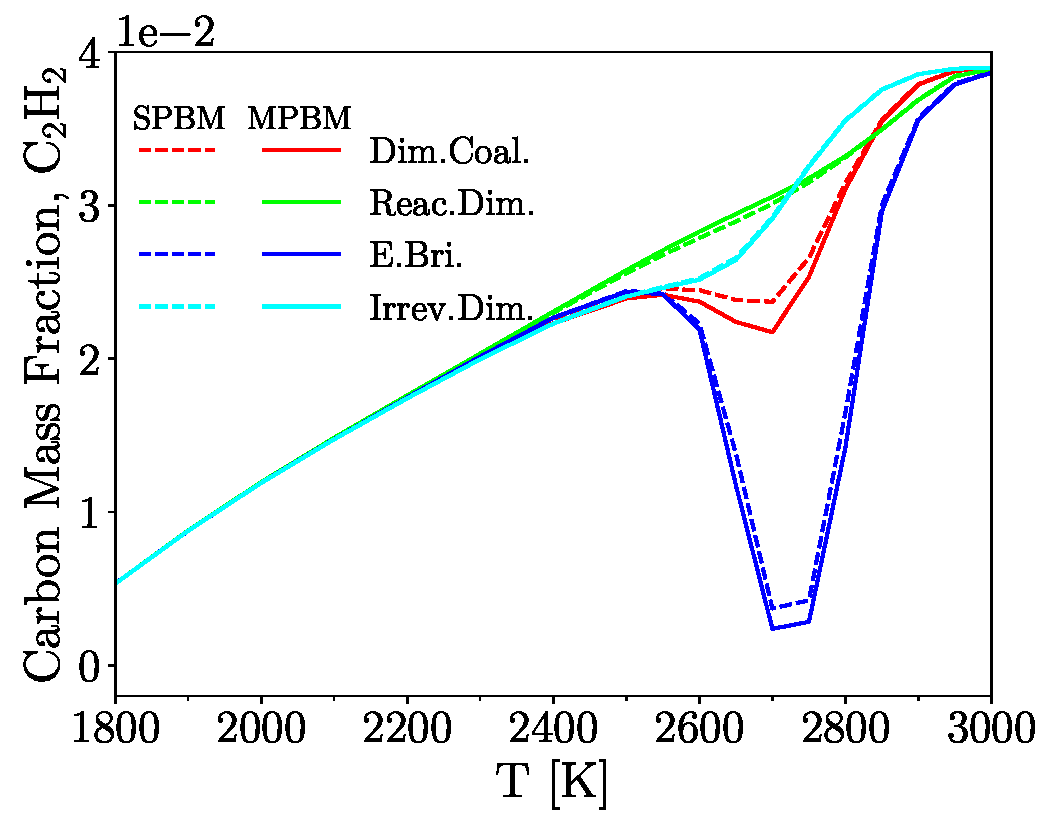
\includegraphics[width=1\textwidth]{Figures/Results/Shocktube/Agafonov2016/10CH4/C2H2.pdf}
	\end{subfigure}
	\caption{The temperature dependence of carbon mass fraction of $\mathrm{C_2H_2}$ during pyrolysis of 5\%~$\mathrm{CH_4}$-Ar (left pane) and 10\%~$\mathrm{CH_4}$-Ar (right pane) at $\mathrm{P}$ = 4.5–6.7 bar obtained using Caltech mechanism and different inception models at t=1.5 ms}
	\label{fig:shocktubeC2H2} 
\end{figure}

Although soot yield, and precursor and acetylene CMF are not sensitive to particle dynamics model, there is a significant difference in agglomerate morphology between SPBM and MPBM predictions. Fig.~\ref{fig:shocktubenp} shows the average number of primary particles per agglomerate, which is larger for SPBM by the maximum factor of 5 for EBridge Formation and Dimer Coalescence in 10\%~$\mathrm{CH_4}$. SPBM predicts larger agglomerates due to accounting for polydispersity of particles that results in higher overall collision rate and faster growth by coagulation. $\mathrm{n_p}$ follows a bell-shape trend similar to soot yield (Fig.~\ref{fig:shocktubeyield}). The $\mathrm{n_p}$ values and the difference between the particle dynamics models reaches their maximum in 2200-2400 K for \%5 $\mathrm{CH_4}$ and 2600-2800 K for \%10 $\mathrm{CH_4}$ because of a stronger inception flux leading to larger number concentration of particles and higher coagulation rate. $\mathrm{n_p}$ is larger for Dimer Coalescence and EBridge Formation reaching the maximum of nearly 100 and 1000 in \%5 and \%10 $\mathrm{CH_4}$, respectively using SPBM. The effect of particle dynamics is minimum for Reactive and Irreversible Dimerization at 5\%~$\mathrm{CH_4}$ over the whole temperature range. 

Fig.\ref{fig:shocktubesigma} shows the standard geometric deviation of mobility diameter, $\mathrm{\sigma_{g}}$ obtained by SPBM that reaches the maximum of 5 and 10 for \%5 and \%10 $\mathrm{CH_4}$, respectively indicating a significant degree of polydispersity in the generated particles at t=1.5ms.

%plot sigma in time to see how it changes and why the sigma values are so large + compare sigma with values from the flame

\begin{figure}[H]
	\centering
	\begin{subfigure}[t]{0.4\textwidth}
		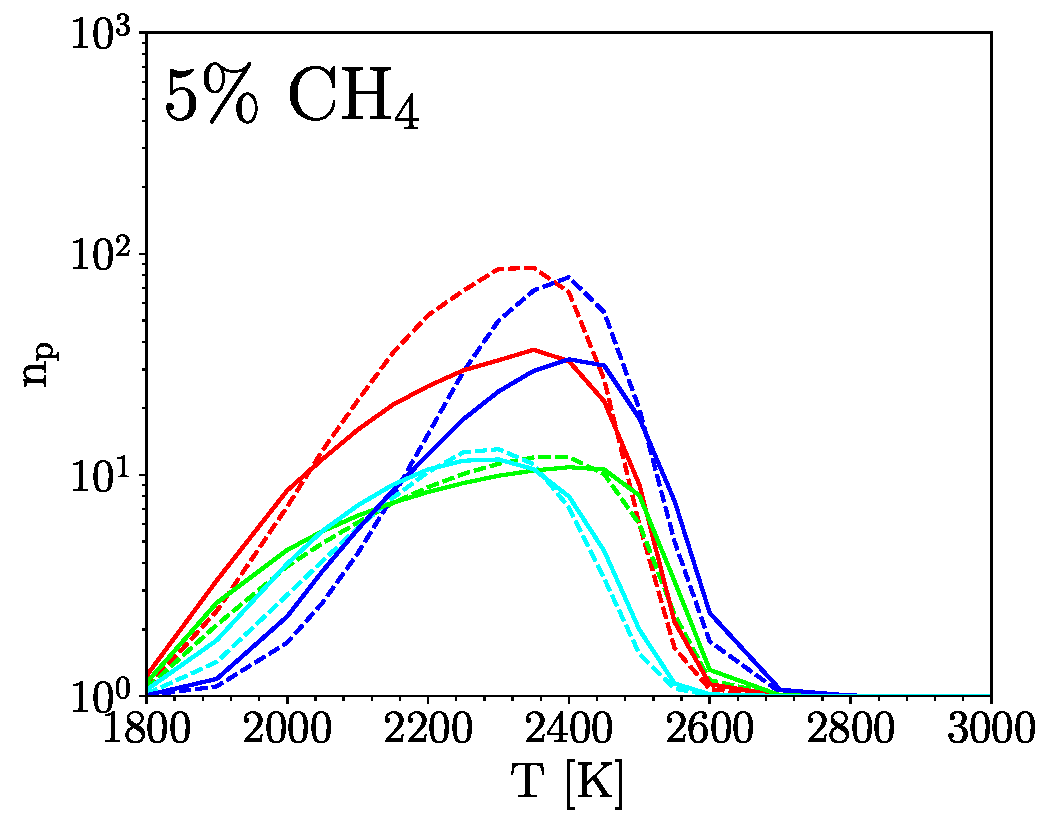
\includegraphics[width=1\textwidth]{Figures/Results/Shocktube/Agafonov2016/5CH4/n_p.pdf}
	\end{subfigure}
	\begin{subfigure}[t]{0.4\textwidth}
		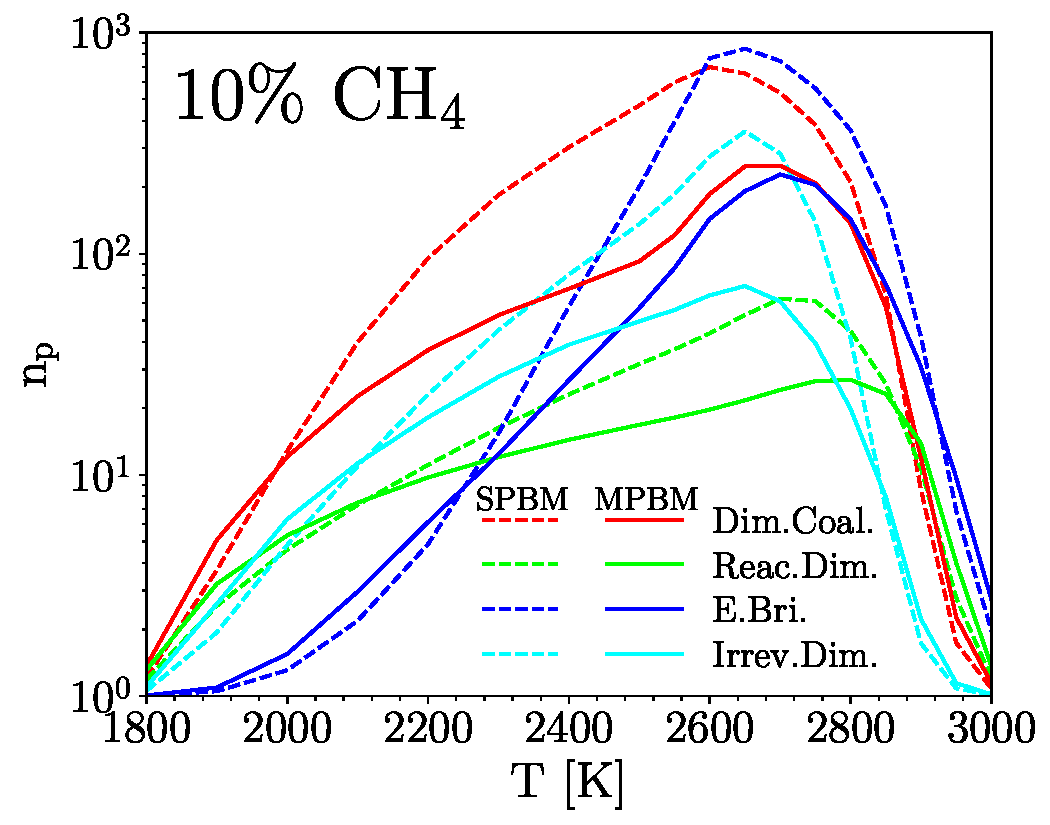
\includegraphics[width=1\textwidth]{Figures/Results/Shocktube/Agafonov2016/10CH4/n_p.pdf}
	\end{subfigure}
	\caption{The temperature dependence of average number of primary particle per agglomerate, $\mathrm{n_p}$ during pyrolysis of 5\%~$\mathrm{CH_4}$-Ar (left pane) and 10\%~$\mathrm{CH_4}$-Ar (right pane) at $\mathrm{P}$ = 4.5–6.7 bar obtained using Caltech mechanism and different inception models at t=1.5 ms}
	\label{fig:shocktubenp} 
\end{figure}

\begin{figure}[H]
	\centering
	\begin{subfigure}[t]{0.4\textwidth}
		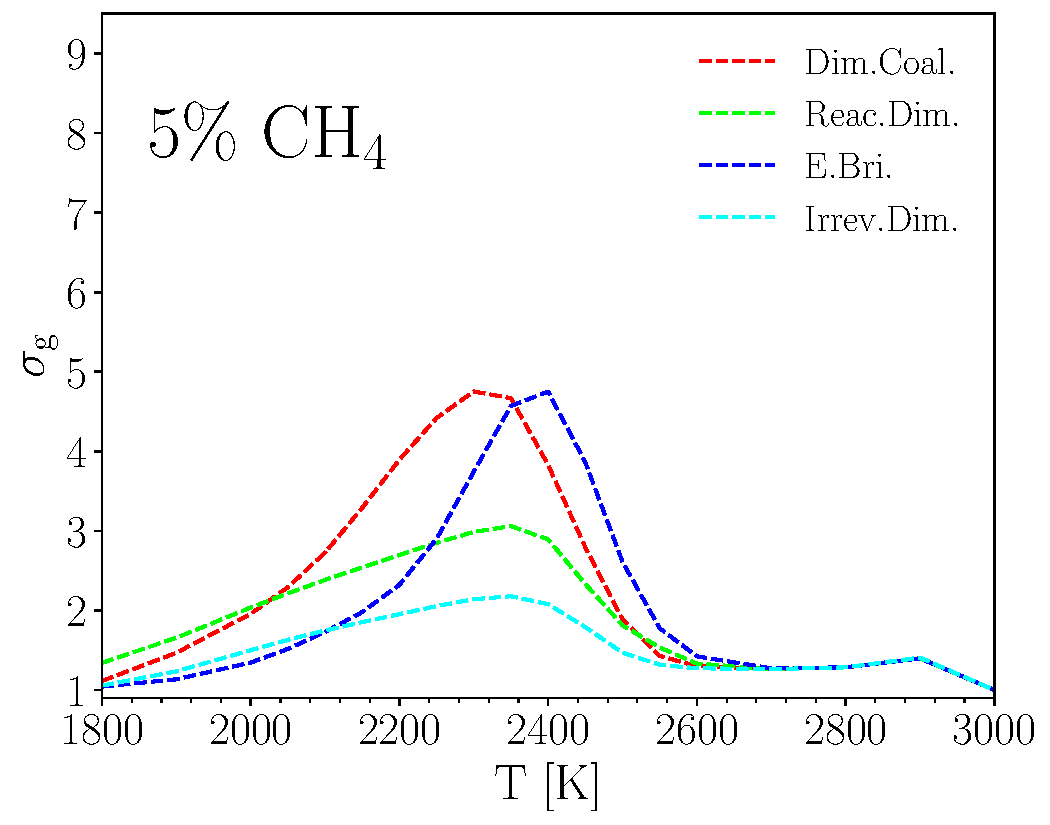
\includegraphics[width=1\textwidth]{Figures/Results/Shocktube/Agafonov2016/5CH4/sigma.pdf}
	\end{subfigure}
	\begin{subfigure}[t]{0.4\textwidth}
		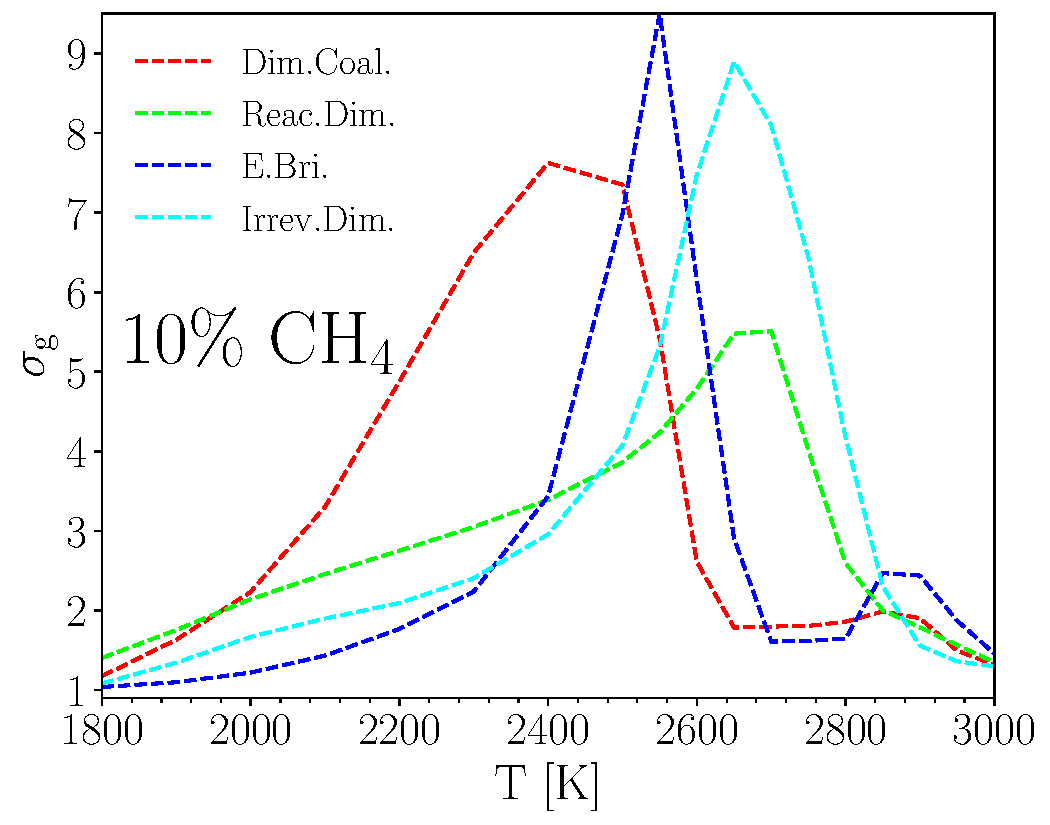
\includegraphics[width=1\textwidth]{Figures/Results/Shocktube/Agafonov2016/10CH4/sigma.pdf}
	\end{subfigure}
	\caption{The time variation of standard geometric deviation of mobility diameter, $\mathrm{\sigma_{g}}$ during pyrolysis of 5\%~$\mathrm{CH_4}$-Ar (left pane) and 10\%~$\mathrm{CH_4}$-Ar (right pane) at $\mathrm{P}$ = 4.5–6.7 bar obtained using Caltech mechanism and different inception models at t=1.5 ms}
\label{fig:shocktubesigma} 
\end{figure}

The $\mathrm{\sigma_{g}}$ values from the SMPS measurements of soot particles at t$\approx$=45ms in a benchmark burner-stabilized premixed are close to 1.1, which is significantly lower than values observed here. So, the evolution of $\mathrm{\sigma_{g}}$ in the studied shock tube is examined in an extended time frame up to 4 msf for 10\%~$\mathrm{CH_4}$ at T=2500 and 2700 K. As shown in Fig.\ref{fig:shocktubesigmatime}, for all PAH growth models $\mathrm{\sigma_{g}}$ rises in the beginning due to simultaneous inception and coagulation that increases polydispersity and rapidly drops and approaches 1.5 before t=3ms when coagulation becomes dominant and inception weaken due to consumption of precursors by PAH adsorption and HACA.


\begin{figure}[H]
	\centering
	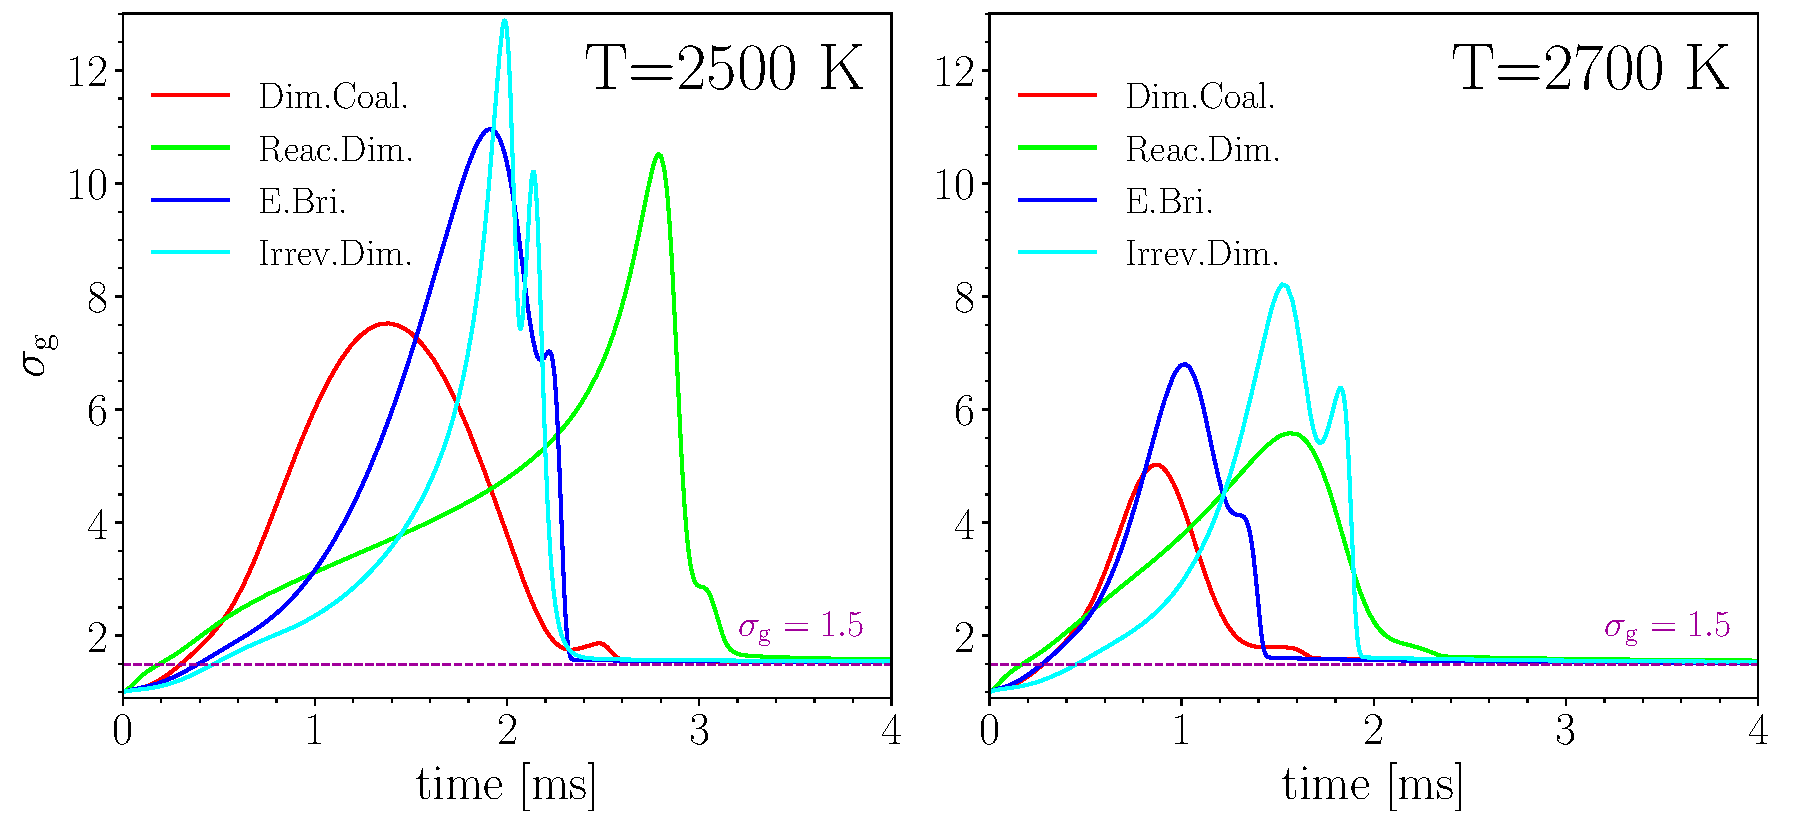
\includegraphics[width=0.8\textwidth]{Figures/Results/Shocktube/Agafonov2016/10CH4/sigma_time.pdf}
	\caption{The temperature dependence of standard geometric deviation of mobility diameter, $\mathrm{\sigma_{g}}$ during pyrolysis of 10\%~$\mathrm{CH_4}$-Ar at T=2500 K (left pane) and T=2700 K (right pane)}
	\label{fig:shocktubesigmatime} 
\end{figure}
%----------------------------------------------------------------
%
% STANFORD SHOKCTUBE DATA 30% CH4
%
%----------------------------------------------------------------

\subsection{Methane pyrolysis data of Stanford (Hanson Group)}

The next set of shock tube data comes from experiments on $\mathrm{CH_4}$ pyrolysis conducted by Ronald Hanson Group at Stanford University. The data has not been published yet (at the time of writing the document) and were provided through the collaboration with Monolith Materials and Stanford University.

The first data set includes eight measurements with the fuel loading of 30\% $\mathrm{CH_4}$-Ar at P=4$\pm$0.5 atm in the temperature range of 1800-2500 K. Table~\ref{tab:shocktubest_CH4_30} lists the process conditions including pressure, temperature and composition of all data points of 30\% $\mathrm{CH_4}$ pyrolysis.


\begin{table}[]
	\caption{The pressure, temperature and composition of simulation data points for 10\% $\mathrm{CH_4}$}
	\centering
	\begin{tabular}{l|llllllll|}
		\cline{2-9}
     	& \multicolumn{8}{c|}{Datapoints}                       \\ \cline{2-9} 
		& (1)  & (2)  & (3)  & (4)  & (5)  & (6)  & (7)  & (8)  \\ \hline
		\multicolumn{1}{|l|}{T {[}K{]}}   & 1861 & 1917 & 2030 & 2155 & 2184 & 2313 & 2375 & 2455 \\ \hline
		\multicolumn{1}{|l|}{P {[}atm{]}} & 4.12 & 3.74 & 3.56 & 3.93 & 3.62 & 3.58 & 3.75 & 3.47 \\ \hline
		\multicolumn{1}{|l|}{Composition} & \multicolumn{8}{c|}{$\mathrm{CH_4}$: 0.3, Ar: 0.7}               \\ \hline
	\end{tabular}
	\label{tab:shocktubest_CH4_30} 
\end{table}

 The time history of $\mathrm{CH_4}$, $\mathrm{C_2H_4}$ and $\mathrm{C_2H_2}$ mole fraction as well as soot yield and volume fraction were reported up to 0.5 ms. Soot volume fraction was measured using light extinction at $\mathrm{\lambda}$=632 nm with E(m)=0.37~\citep{agafonov2015soot}. The constant volume reactor was used with all PAH growth and particle dynamics models. First, the effect of gas chemistry on species and soot predictions will be examined by comparing the temperature, mole fraction of $\mathrm{CH_4}$, $\mathrm{C_2H_2}$ and soot volume fraction obtained using Caltech~\citep{blanquart2009chemical}, KAUST~\cite{wang2013pah} and ABF~\citep{appel2000kinetic} reaction mechanisms. Here, the comparison is done for one data point, T=2184 K and P=3.62 atm, but the extensive investigations in Appendix\hl{****} shows that the conclusions about the mechanisms are valid for the entire data set. Fig.\ref{fig:shocktubestT} temperature time history predicted by different PAH growth and particle dynamics models and mechanisms. All mechanisms underpredict the temperature and the discrepancy between numerical results and measurements increases with time. While the error of ABF predictions reaches a maximum of 33 K at t=0.5 ms, which is with acceptable range considering the experimental uncertainties, KAUST and Caltech yield the maximum error of 60 K and 102 K at the same time, respectively. As shown in Fig.\ref{fig:shocktubestch4} and \ref{fig:shocktubestch4}, ABF mechanism has a more accurate prediction of mole fraction of $\mathrm{CH_4}$ and $\mathrm{C_2H_2}$, but Caltech and KAUST uderpredict both quantities indicating that these mechanisms predict a stronger  decomposition rate of $\mathrm{CH_4}$ and a higher conversion of $\mathrm{C_2H_2}$ to larger hydrocarbons, especially PAHs. 

\begin{figure}[H]
	\centering
	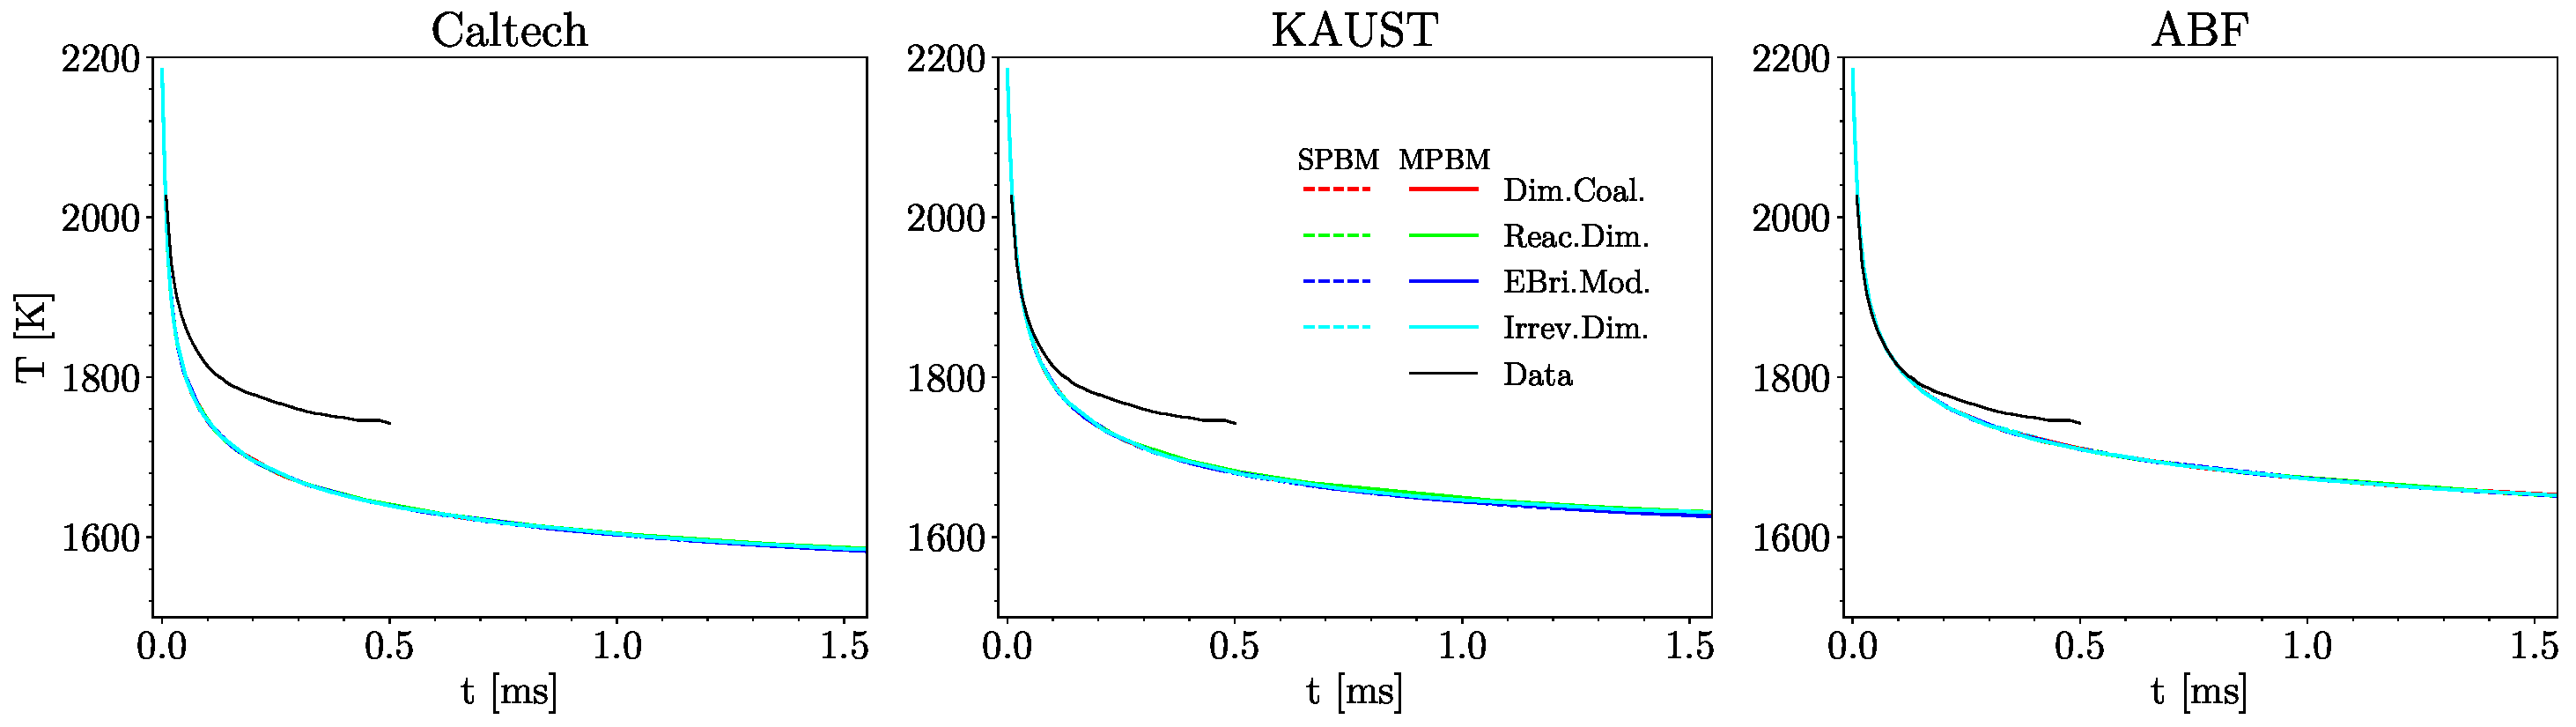
\includegraphics[width=0.9\textwidth]{Figures/Results/Shocktube/Stanford/june/stsh_mech_compare_T.pdf}
	\caption{The time history of temperature of 30\% $\mathrm{CH_4}$ pyrolysis at T=2184 K and P=3.62 atm using Caltech, KAUST, and ABF mechanism and different PAH growth and particle dynamics models}
	\label{fig:shocktubestT} 
\end{figure}

\begin{figure}[H]
	\centering
	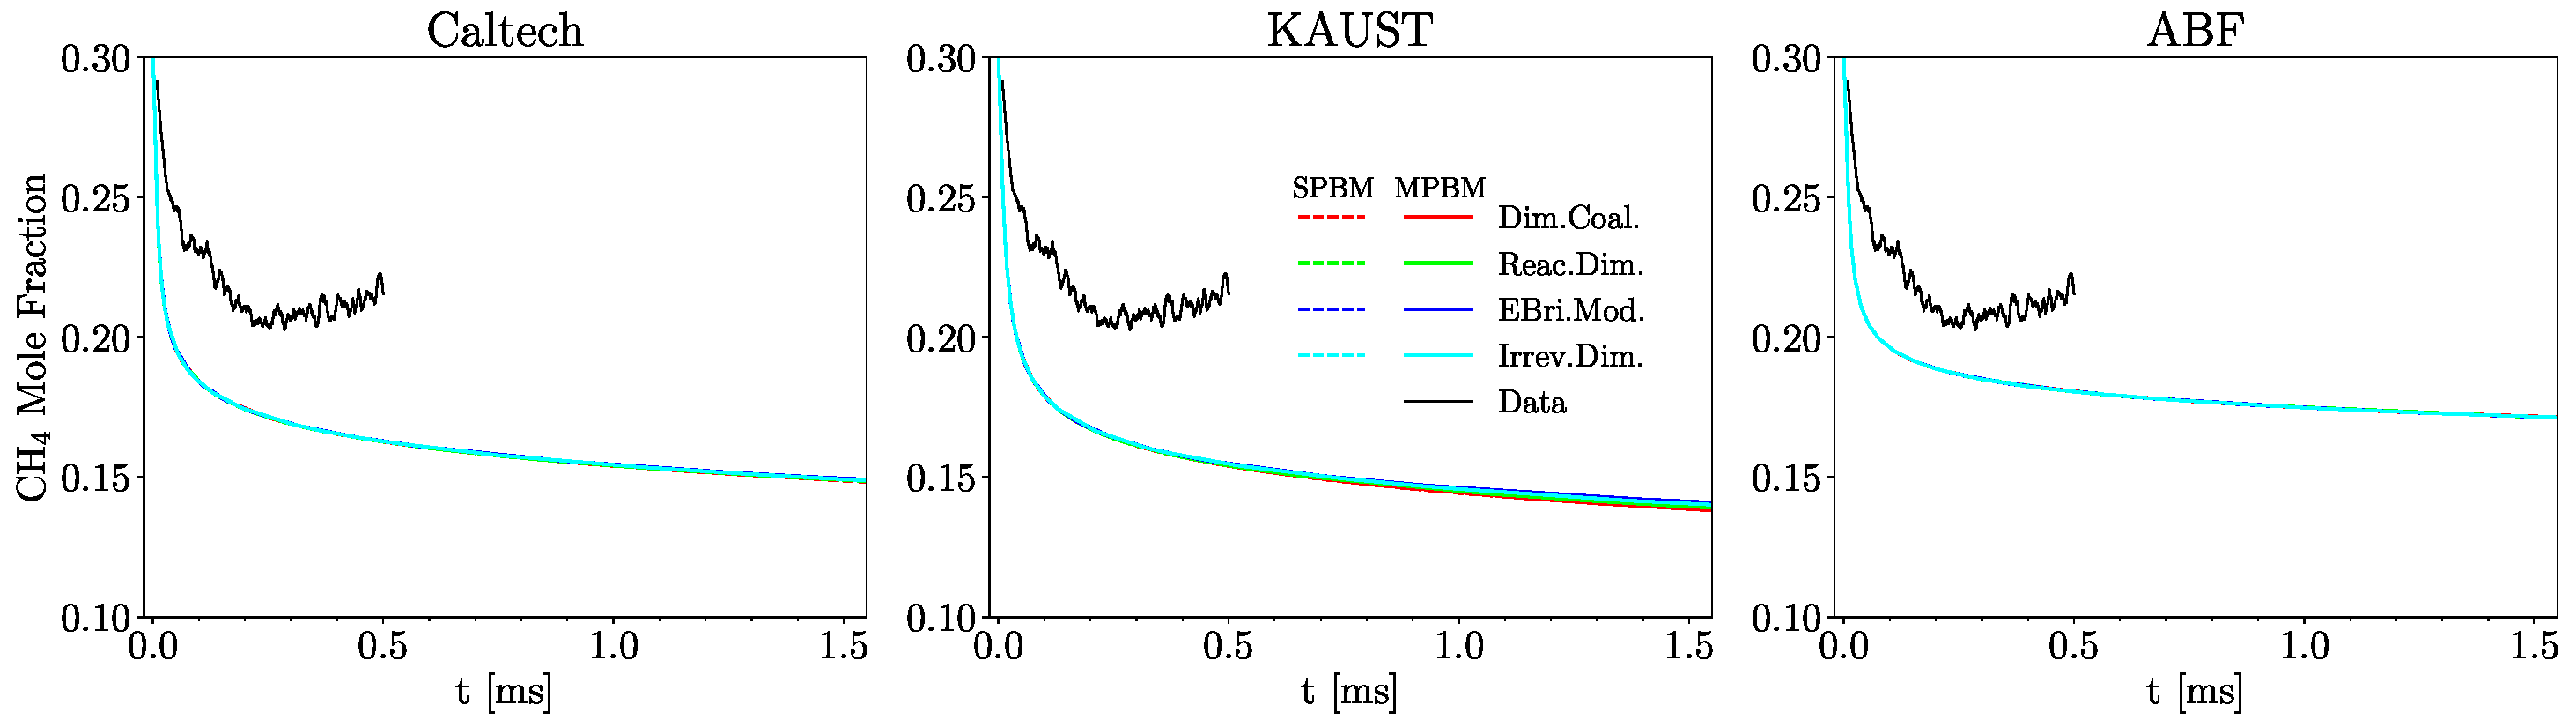
\includegraphics[width=0.9\textwidth]{Figures/Results/Shocktube/Stanford/june/stsh_mech_compare_CH4.pdf}
	\caption{The time history of $\mathrm{CH_4}$ mole fraction of 30\% $\mathrm{CH_4}$ pyrolysis at T=2184 K and P=3.62 atm using Caltech, KAUST, and ABF mechanism and different PAH growth and particle dynamics models}
	\label{fig:shocktubestch4} 
\end{figure}

\begin{figure}[H]
	\centering
	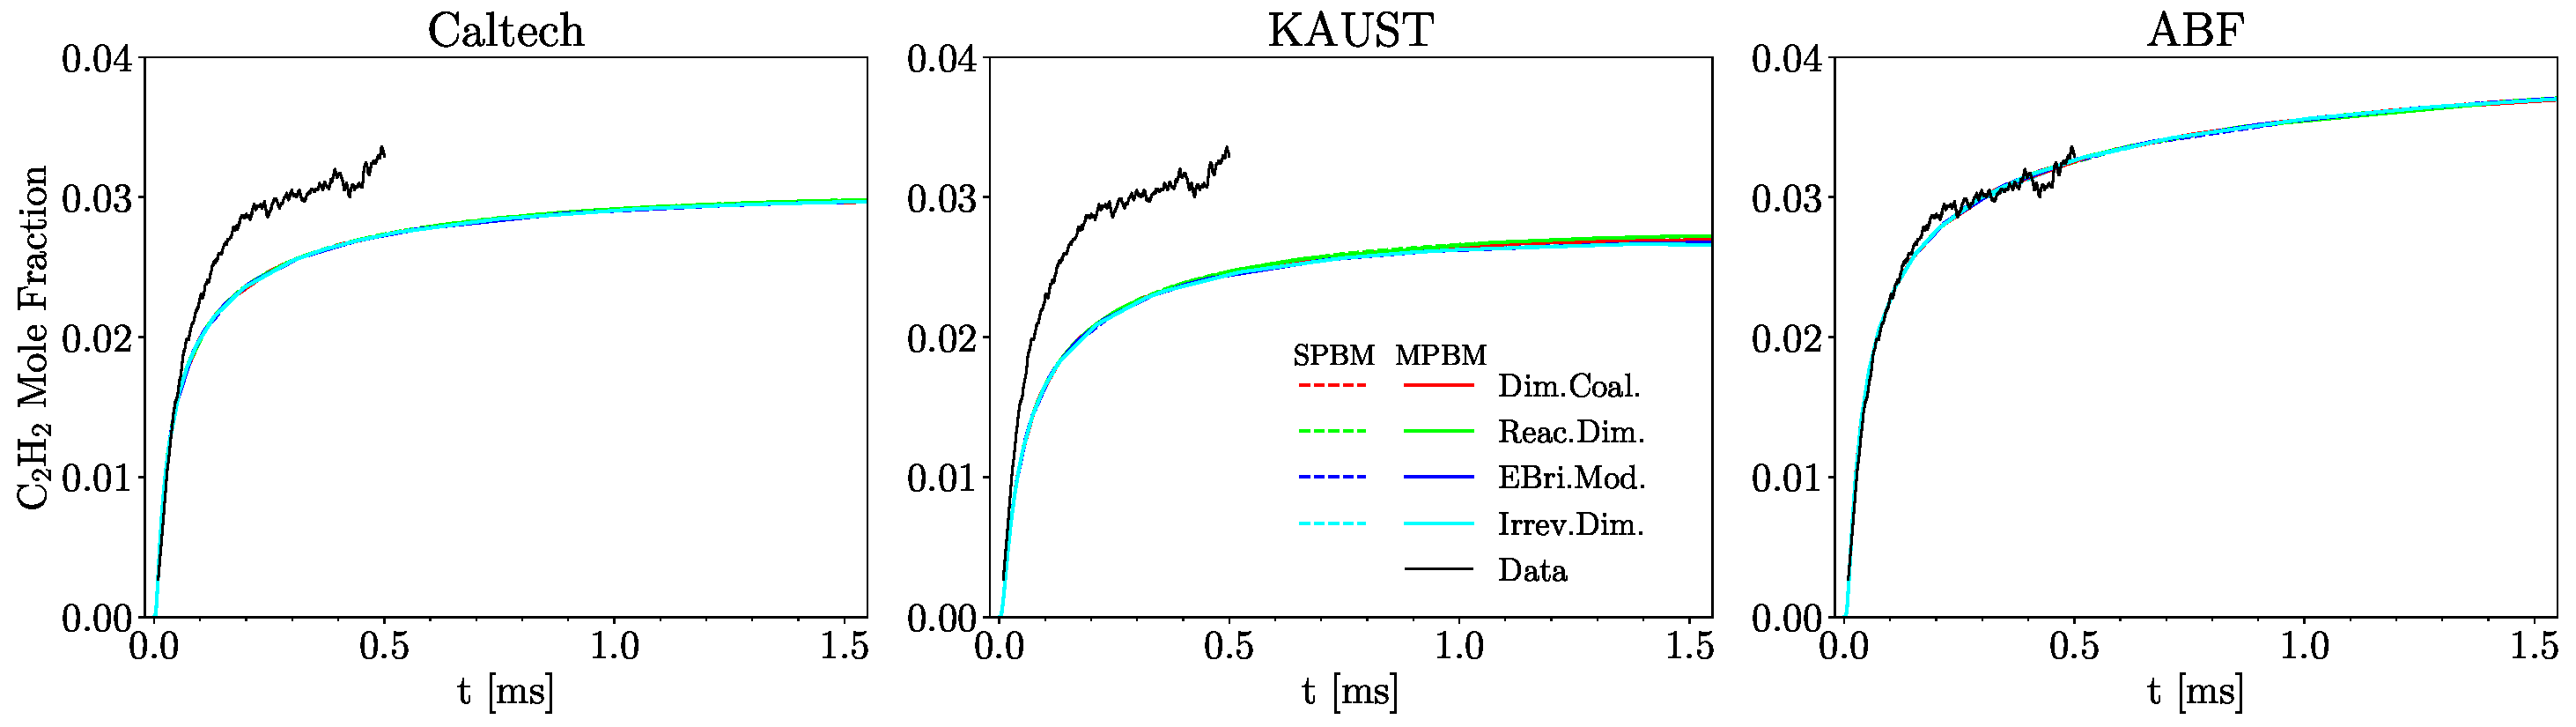
\includegraphics[width=0.9\textwidth]{Figures/Results/Shocktube/Stanford/june/stsh_mech_compare_C2H2.pdf}
	\caption{The time history of $\mathrm{C_2H_2}$ mole fraction of 30\% $\mathrm{CH_4}$ pyrolysis at T=2184 K and P=3.62 atm using Caltech, KAUST, and ABF mechanism and different PAH growth and particle dynamics models}
	\label{fig:shocktubestc2h2} 
\end{figure}

This is better evident in Fig.~\ref{fig:shocktubestch4} showing CMF of $\mathrm{CH_4}$, $\mathrm{C_2H_4}$, and $\mathrm{C_2H_2}$ combined. The results obtained using ABF increases after the initial decrease varying in the range of 1-0.95 indicating that most of carbon mass ($>$95\%) remains in these three species in the studied time frame. However, CMF of the species continuously decreases with KAUST and Caltech confirming the lack/weakness of pathways driving the transfer of carbon from small to large hydrocarbon in ABF mechanism that significantly reduces the soot inception rates. Fig.~\ref{fig:shocktubestvf} shows the soot volume fraction predicted using different models and mechanisms. ABF underpredicts $f_v$ by more than three orders of magnitude, but KAUST and Caltech predictions are close, for some PAH growth models, exceeds the measurements. Interestingly, the combination of KAUST and Ebridge Formation perfectly matches the value and trend of experimental $f_v$. The mechanism comparison can be summarized as following: ABF mechanism predict more accurate temperature and the mole fraction of $\mathrm{CH_4}$ and $\mathrm{C_2H_2}$, but remarkably underestimates soot volume fraction due to a low production rate of PAHs from $\mathrm{C_2H_2}$. Caltech and KAUST overestimate the endothermic decomposition of $\mathrm{CH_4}$ leading to lower temperature prediction, and directs more carbon to PAHs resulting in comparable soot mass. The temperature and species mole fractions is not sensitive to PAH growth and particle dynamics models. $f_v$ significantly changes with PAH growth model, but MPBM and SPBM predictions overlap within 1.5 ms of the simulation. As a results, only simulations by KAUST are used to examine soot morphology and composition and the effect of PAH growth models in the temperature range. 

\begin{figure}[H]
	\centering
	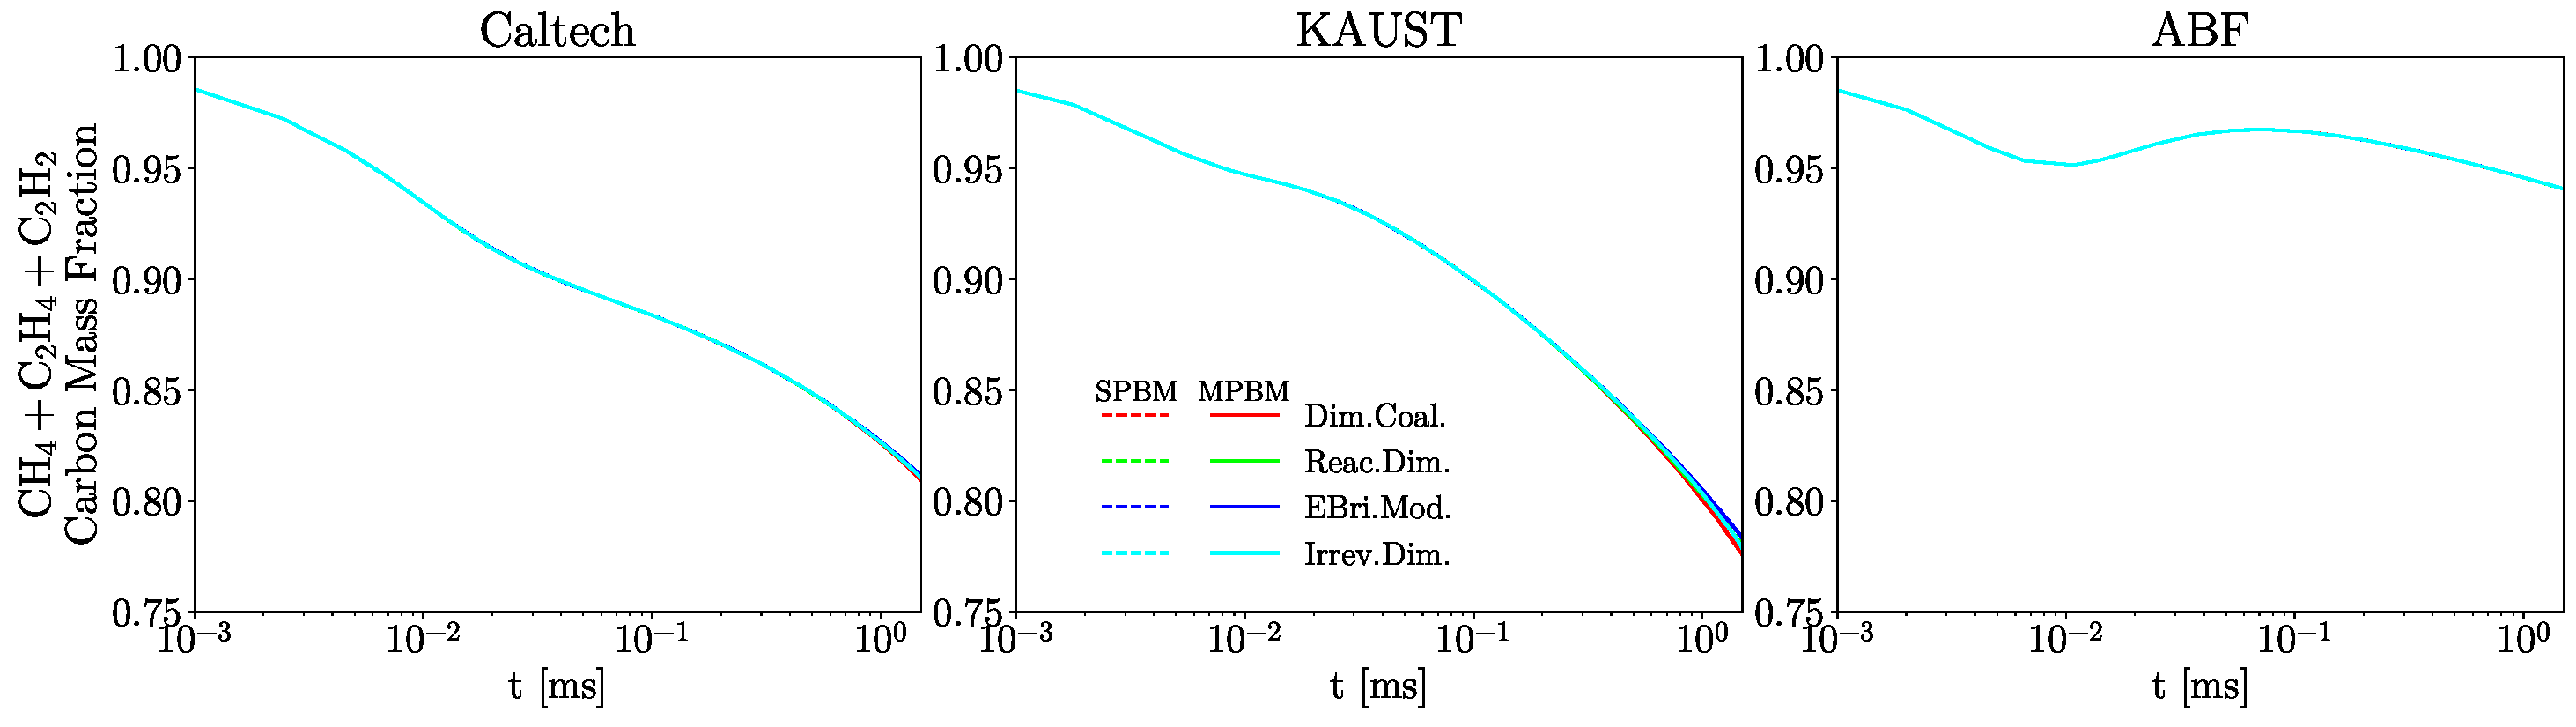
\includegraphics[width=0.9\textwidth]{Figures/Results/Shocktube/Stanford/june/stsh_mech_compare_CCC.pdf}
	\caption{The time history of carbon mass fraction of $\mathrm{CH_4}$, $\mathrm{C_2H_4}$, and $\mathrm{C_2H_2}$ of 30\% $\mathrm{CH_4}$ pyrolysis at T=2184 K and P=3.62 atm using Caltech, KAUST, and ABF mechanism and different PAH growth and particle dynamics models}
	\label{fig:shocktubestccc} 
\end{figure}


\begin{figure}[H]
	\centering
	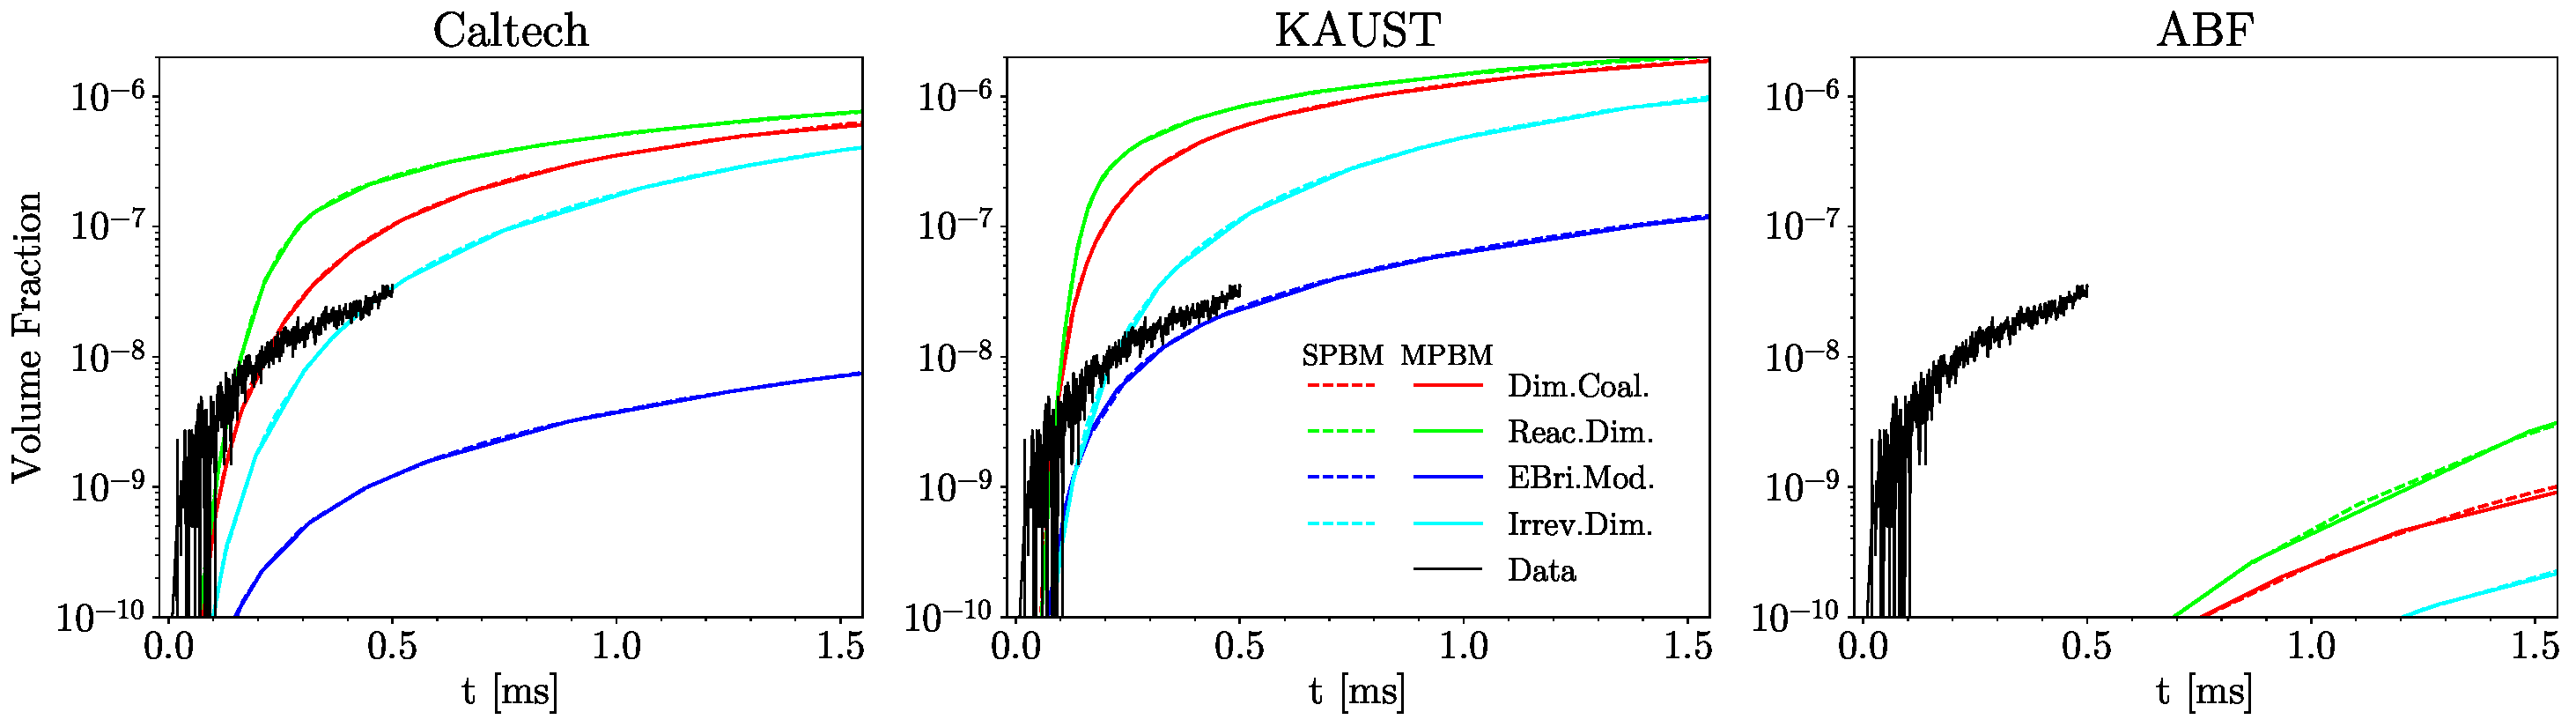
\includegraphics[width=0.9\textwidth]{Figures/Results/Shocktube/Stanford/june/stsh_mech_compare_vf.pdf}
	\caption{The time history of soot volume fraction of 30\% $\mathrm{CH_4}$ pyrolysis at T=2184 K and P=3.62 atm using Caltech, KAUST, and ABF mechanism and different PAH growth and particle dynamics models}
	\label{fig:shocktubestvf} 
\end{figure}

Fig.~\ref{fig:shocktubestcasevf} shows that the time variation of soot volume fraction in the temperature range of 1800-2500 K. The measurement data was not available (or too noisy) below T=2155 K due to lack of enough soot particle leading to weak extinction signal. In all cases with higher temperatures, EBridge Formation predicts the lowest volume fraction that interestingly are in close agreement with the data. Reactive Dimerization and Dimer Coalescence yields the largest $f_v$ nearly two orders of magnitude higher than the measurements that start with a rapid increase indicating a stronger inception rate leading to larger number concentration of particles that provide more surface area for surface growth via HACA. Shock tube temperature increases $f_v$ with all PAH growth models over the 1.5 ms. Moreover, high temperature accelerates soot formation, which can be examined by comparing $f_v$ at early stages of simulation. For example, no soot appears before t=0.25 ms i.e. $f_v<10^{-10}$ at T=1861 K, but $f_v$ approaches $10^{-6}$ at T=2455.

Fig.\ref{fig:shocktubestcasedp} shows the time history of primary particle diameter, $d_p$ at different temperatures. As expected, EBridge Formation and Irreversible Dimerization has the lowest $d_p$ due to low soot mass growth rate leading to small $f_v$ values. Although Dimer Coalescence and Reactive Dimerization generate close volume fraction values corresponding to similar soot mass, the latter predicts larger $d_p$ indicating a lower number of $N_{pri}$. In other words, RD has lower inception rates and a stronger PAH adsorption rate compared to DC. The $d_p$ by RD exhibits a noticeable sensitivity to particle dynamics model that grows with temperature. Both model predict the initial rapid rise in $d_p$. While MPBM predicts a gradual increase to final value, $d_p$ by SPBM decreases for T$>$2000 K due to stronger inception rate by SPBM that generates particle with $d_p$=2 nm bringing down the average $d_p$.

% Final fv in terms of temperature
% the time that it taks for each PAH growth model to each 50%/90% of the final value

\begin{figure}[H]
	\centering
	\includegraphics[width=1\textwidth]{Figures/Results/Shocktube/Stanford/june/stsh_cases_vf.pdf}
	\caption{The time history of soot volume fraction of 30\% $\mathrm{CH_4}$ pyrolysis in the temperature range of 1800-2500 K and P=4$\pm$0.5 atm using KAUST mechanism and different PAH growth and particle dynamics models}
	\label{fig:shocktubestcasevf} 
\end{figure}


\begin{figure}[H]
	\centering
	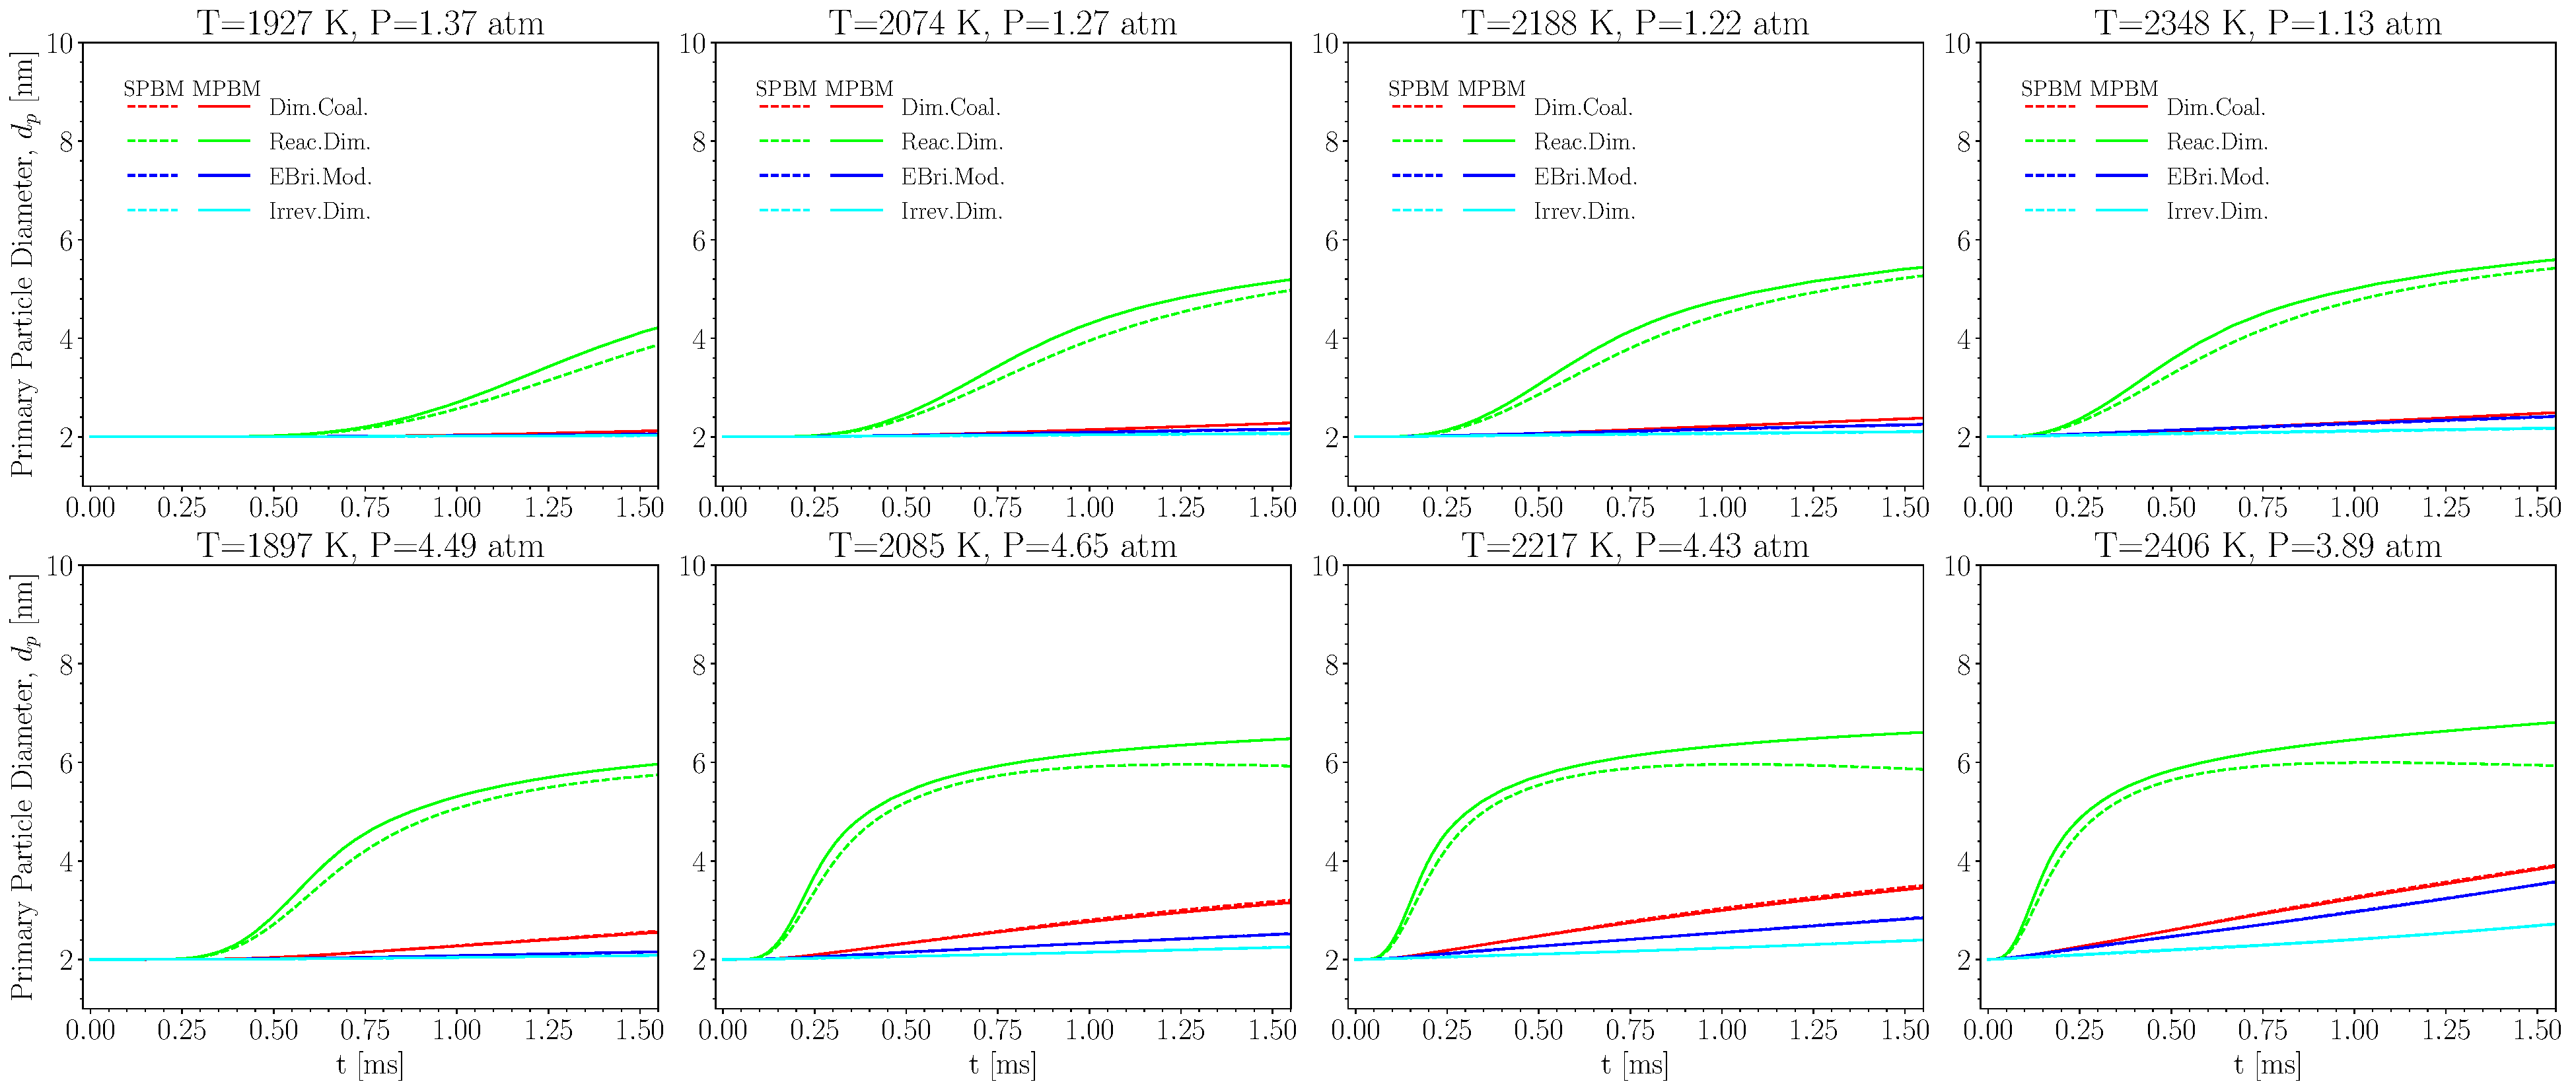
\includegraphics[width=1\textwidth]{Figures/Results/Shocktube/Stanford/june/stsh_cases_dp.pdf}
	\caption{The time history of primary particle diameter, $d_p$ of 30\% $\mathrm{CH_4}$ pyrolysis in the temperature range of 1800-2500 K and P=4$\pm$0.5 atm using KAUST mechanism and different PAH growth and particle dynamics models}
	\label{fig:shocktubestcasedp} 
\end{figure}

Fig.\ref{fig:shocktubestcasedm} shows time histories $d_m$ at different shock tube temperature. Similar to $d_p$, $d_m$ increases over time and with shock tube temperature. The rise in $d_m$ occurs faster. Initially, the generated agglomerates are small ($n_p\approx1$), and $d_m$ is close to $d_p$, so RD yield the highest $d_m$, but DC takes over and exceeds RD. Additionally, $d_m$ predicted by MPBM is larger in the beginning of the simulation, but $d_m$ predicted by SPBM rises faster at longer residence times. Fig.~\ref{fig:shocktubecarbon} shows the carbon mass growth rate by inception, HACA and PAH adsorption at T=2455 K and P=3.47 atm that explains the difference in the behavior of PAH growth and particle dynamics model in prediction of soot mass and morphology. The inception rate of RD (Fig.~\ref{fig:shocktubecarbon}-a) rapidly rises reaching its peak values and quickly drops until t=0.25 ms when a bifurcation occurs. While the inception rate by MPBM gradually decreases, SPBM predicts an increasing rate of production of new particles leading to a smaller $d_p$. DC reaches the inception peak higher than other PAH growth models before t=0.25 ms creating more particles that causes larger $d_m$ after coagulation becomes dominant. Such a high number concentration also leads to large HACA growth rates evident in Fig.~\ref{fig:shocktubecarbon}-b. RD has the highest PAH adsorption rate with a peak near t=0.1 ms as opposed to other PAH growth models that causes the rapid drop in inception rate and higher soot mass gain rates leading to larger volume fraction (Fig.\ref{fig:shocktubestvf}).

\begin{figure}[H]
	\centering
	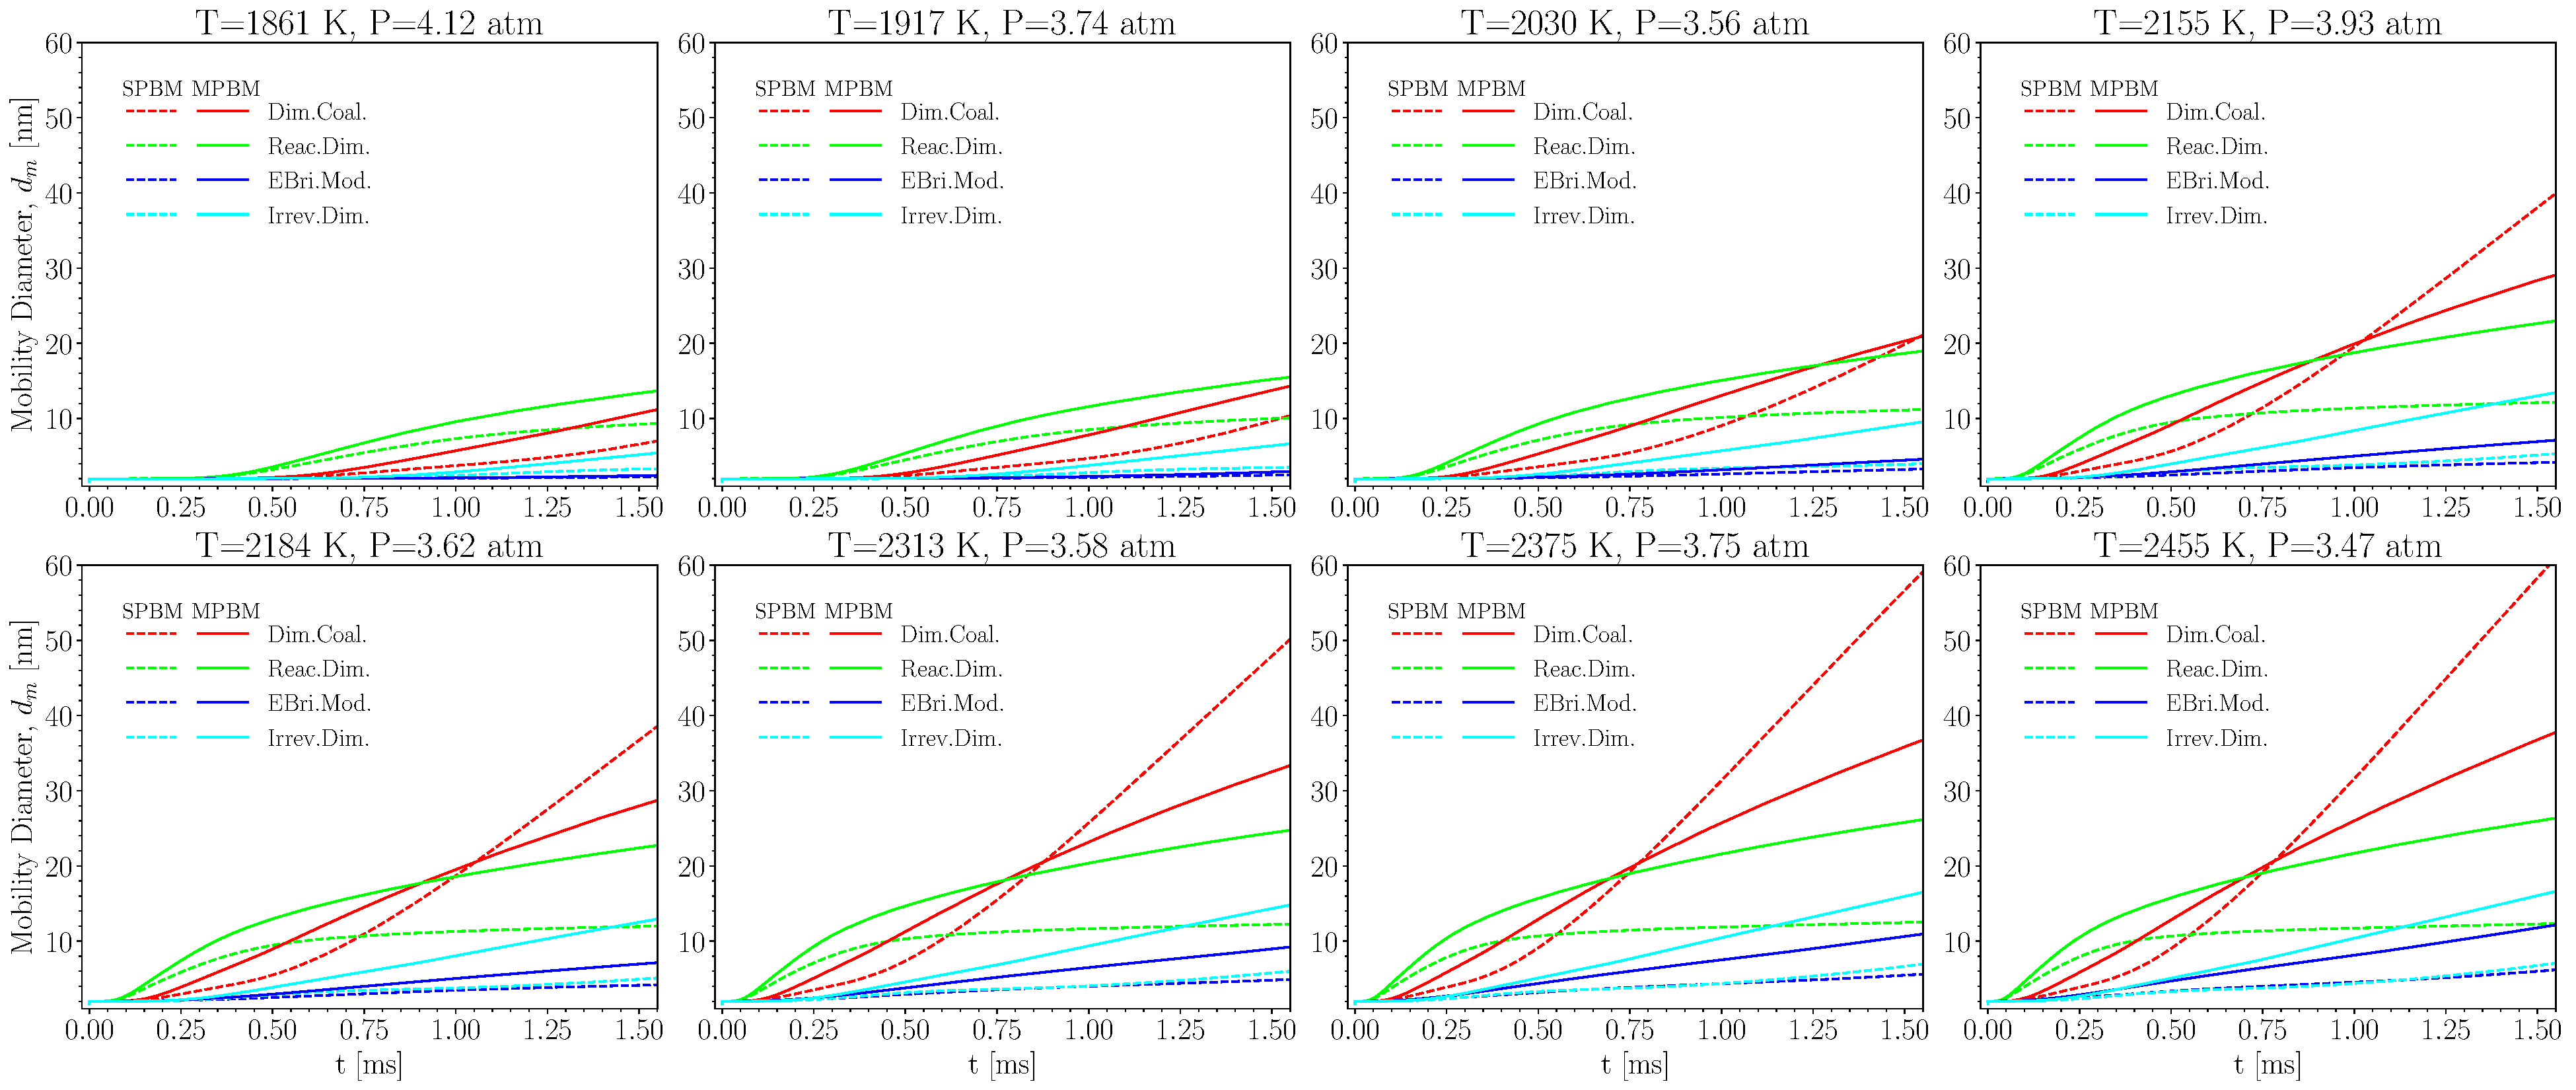
\includegraphics[width=1\textwidth]{Figures/Results/Shocktube/Stanford/june/stsh_cases_dm.pdf}
	\caption{The time history of mobility diameter, $d_m$ of 30\% $\mathrm{CH_4}$ pyrolysis in the temperature range of 1800-2500 K and P=4$\pm$0.5 atm using KAUST mechanism and different PAH growth and particle dynamics models}
	\label{fig:shocktubestcasedm} 
\end{figure}

\begin{comment}
	\begin{figure}[H]
		\centering
		\begin{subfigure}[t]{0.32\textwidth}
			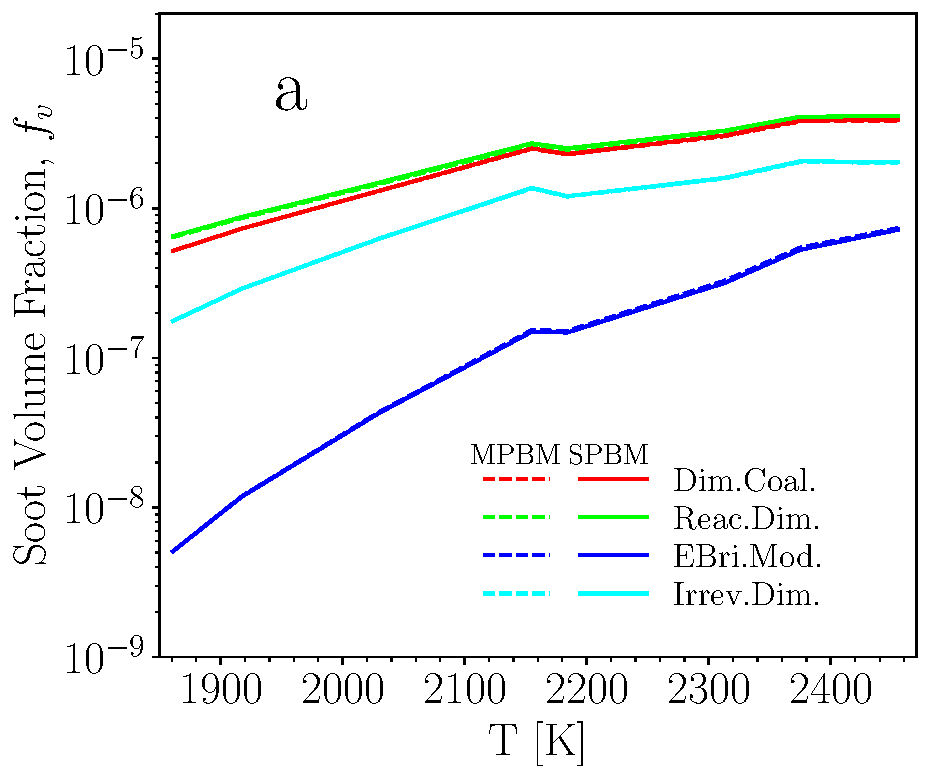
\includegraphics[width=1\textwidth]{Figures/Results/Shocktube/Stanford/June/stsh_temp_fv.pdf}
		\end{subfigure}
		\begin{subfigure}[t]{0.32\textwidth}
			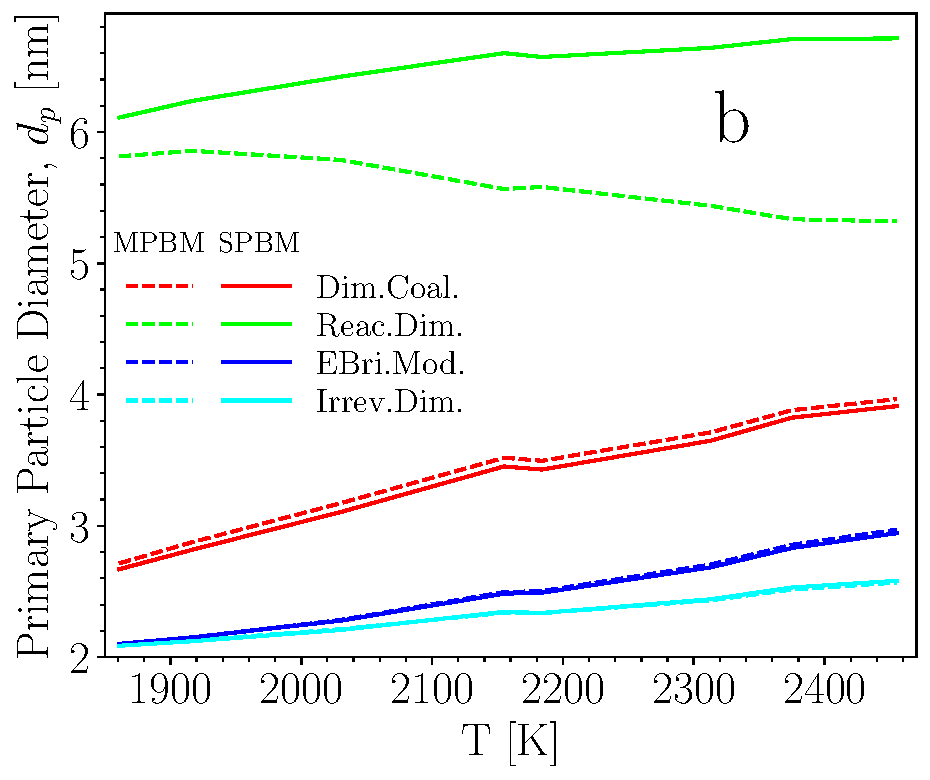
\includegraphics[width=1\textwidth]{Figures/Results/Shocktube/Stanford/June/stsh_temp_dp.pdf}
		\end{subfigure}
		\begin{subfigure}[t]{0.32\textwidth}
			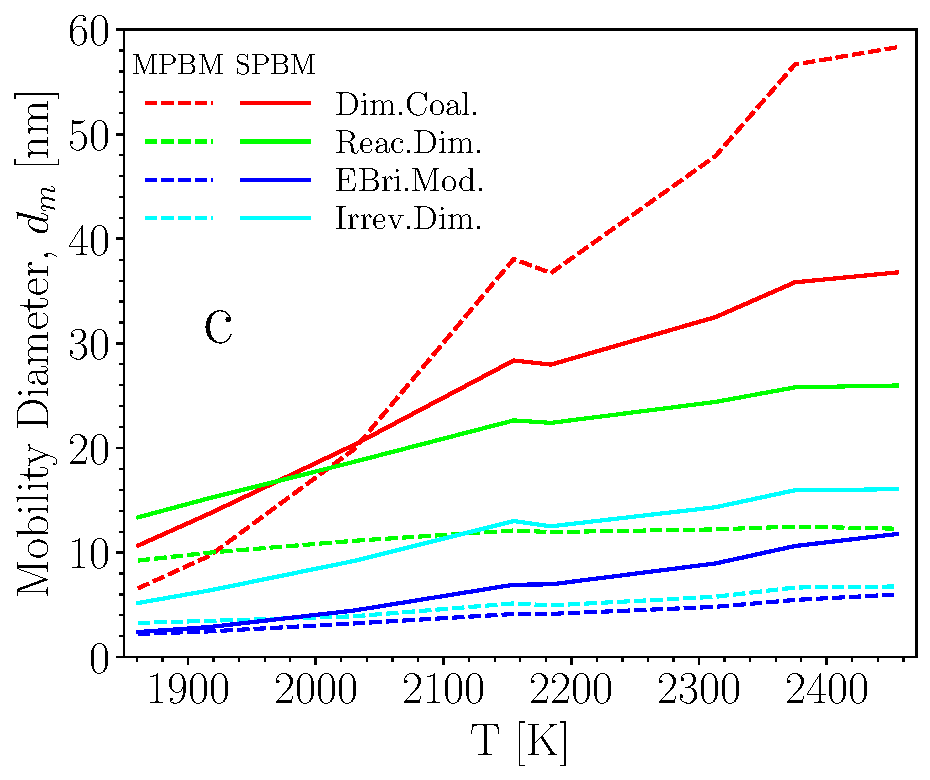
\includegraphics[width=1\textwidth]{Figures/Results/Shocktube/Stanford/June/stsh_temp_dm.pdf}
		\end{subfigure}
		\caption{The temperature dependence of volume fraction, $f_v$ (a), primary particle diameter, $d_p$ (b), mobility diameter, $d_m$ (c) at t=1.5ms of pyrolysis of 30\% $\mathrm{CH_4}$ in the temperature range of 1800-2500 K and P=4$\pm$0.5 atm using KAUST mechanism and different PAH growth and particle dynamics models}
		\label{fig:shocktubetemponehalf} 
	\end{figure}
\end{comment}



\begin{figure}[H]
	\centering
	\begin{subfigure}[t]{0.32\textwidth}
		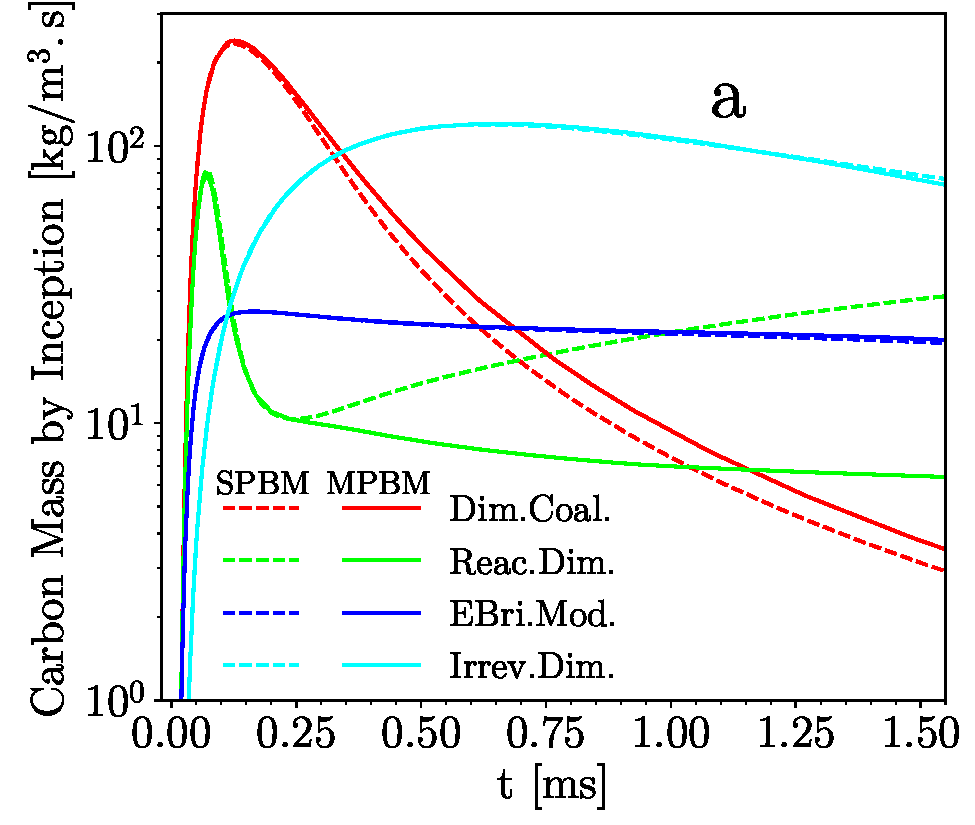
\includegraphics[width=1\textwidth]{Figures/Results/Shocktube/Stanford/June/stsh_single_inc.pdf}
	\end{subfigure}
	\begin{subfigure}[t]{0.32\textwidth}
		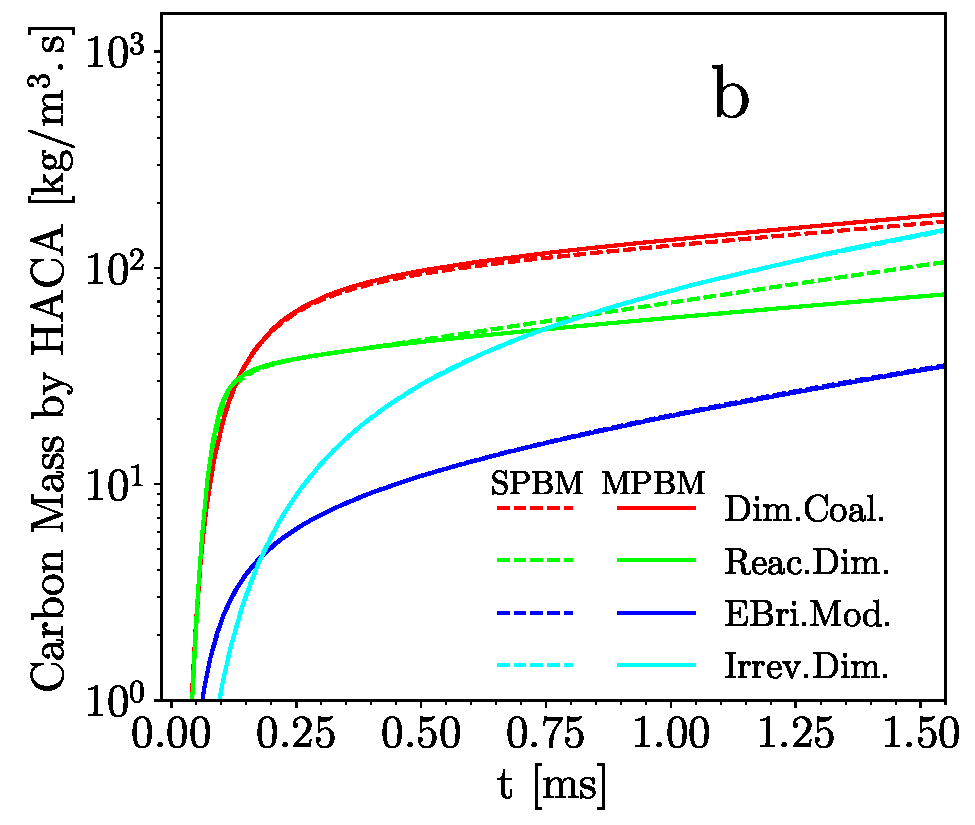
\includegraphics[width=1\textwidth]{Figures/Results/Shocktube/Stanford/June/stsh_single_HACA.pdf}
	\end{subfigure}
	\begin{subfigure}[t]{0.32\textwidth}
		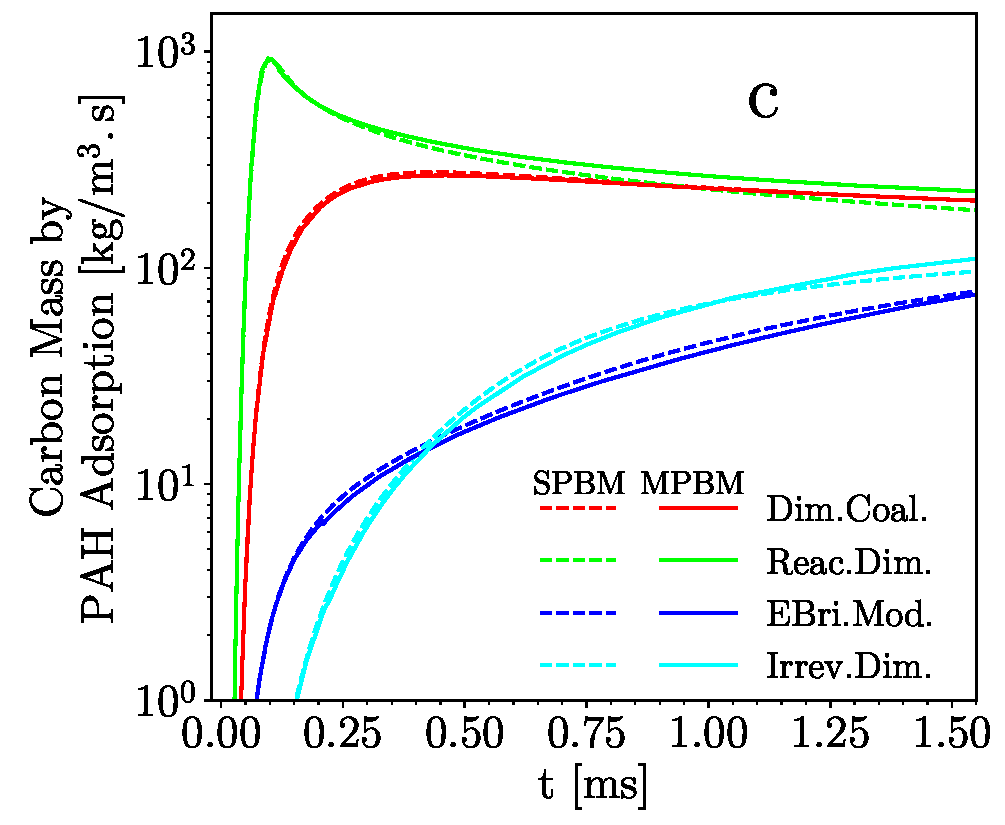
\includegraphics[width=1\textwidth]{Figures/Results/Shocktube/Stanford/June/stsh_single_PAH.pdf}
	\end{subfigure}
	\caption{The time history of carbon mass gained by inception(a), HACA (b), and PAH adsorption (c) of pyrolysis of 30\% $\mathrm{CH_4}$ at T=2455 K and P=3.47 atm using KAUST mechanism and different PAH growth and particle dynamics models}
	\label{fig:shocktubecarbon} 
\end{figure}


%----------------------------------------------------------------
%
% STANFORD SHOKCTUBE DATA 10% CH4
%
%----------------------------------------------------------------

Now, we will examine the data from Stanford's group experiments on 10\% $\mathrm{CH_4}$ pyrolysis at P=1$\pm$0.5 atm and 4$\pm$0.5 atm in the temperature range of 1900-2500 K.


\begin{table}[]
	\caption{The pressure, temperature and composition of simulation data points for 10\% $\mathrm{CH_4}$}
	\centering
	\begin{tabular}{l|llllllll|}
		\cline{2-9}
		& \multicolumn{8}{c|}{Datapoints}                       \\ \cline{2-9} 
		& (1)  & (2)  & (3)  & (4)  & (5)  & (6)  & (7)  & (8)  \\ \hline
		\multicolumn{1}{|l|}{T {[}K{]}}   & 1927 & 2074 & 2030 & 2348 & 1897 & 2085 & 2277 & 2406 \\ \hline
		\multicolumn{1}{|l|}{P {[}atm{]}} & 1.37 & 1.27 & 1.22 & 1.13 & 4.49 & 4.85 & 4.43 & 3.89 \\ \hline
		\multicolumn{1}{|l|}{Composition} & \multicolumn{8}{c|}{$\mathrm{CH_4}$: 0.1, $\mathrm{CO_2}$: 0.01, Ar: 0.7}               \\ \hline
	\end{tabular}
	\label{tab:shocktubest_CH4_10} 
\end{table}


First, the mechanism comparison is conducted by simulating 10\% $\mathrm{CH_4}$ pyrolysis in a constant volume reactor. As shown before in Figs.~\ref{fig:shocktubestch4} and ~\ref{fig:shocktubestc2h2}, the particle dynamics and PAH growth models has minimal effect on the prediction of major small hydrocarbons. So, the mechanism comparison is only based on the combination of MPBM and RD to avoid clutter in graphs, and it is focused on two data points, T=2188 K, P=1.22 atm and T=2217 K, P=4.43 atm, each being representative of atmospheric and high pressure cases, respectively. Fig.\ref{fig:shocktubes_sepch4} shows $\mathrm{CH_4}$ mole fraction for these data points predicted using KAUST, Caltech, and ABF mechanisms and compared with measurements. Similar to 30\% $\mathrm{CH_4}$ data set, KAUST and Caltech yield larger $\mathrm{CH_4}$ conversion corresponding to a lower mole fraction. However, KAUST predictions are in close agreement for both data points, but ABF underestimates $\mathrm{CH_4}$ conversion. As shown in Fig.~\ref{fig:shocktubes_sepc2h2}, all mechanisms exhibit a similar behavior underestimating $\mathrm{C_2H_2}$ mole fraction in the high pressure, but overestimating it for the atmospheric case. Fig.~\ref{fig:shocktubes_sepvf} compares soot volume fraction predicted by different mechanisms with light extinction measurements. As expected, ABF significantly underpredicts $f_v$ due to low production rate of soot precursors (PAHs). Temperature analysis is not done for 10\% $\mathrm{CH_4}$ due to lack of measurements. KAUST mechanism is used for soot analysis as it predicts species and soot volume fraction close to the measurements.

\begin{figure}[H]
	\centering
	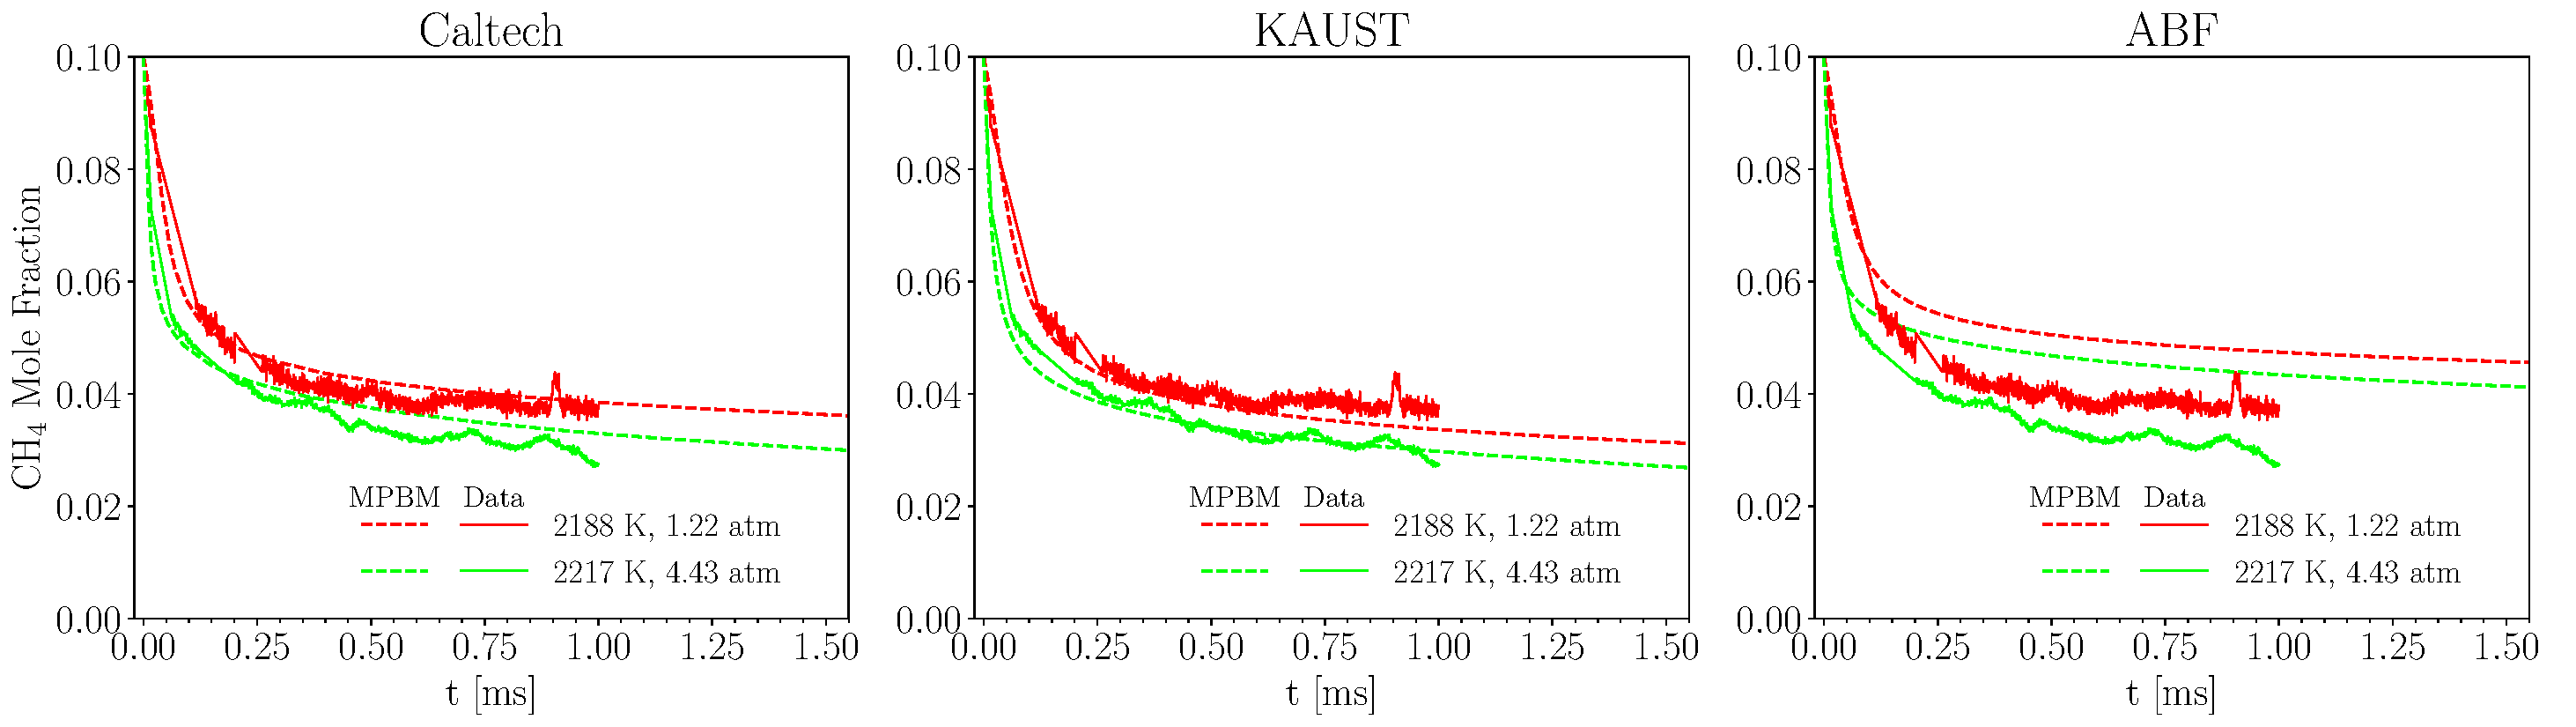
\includegraphics[width=0.9\textwidth]{Figures/Results/Shocktube/Stanford/September/stsh_sepmechs_CH4.pdf}
	\caption{The time history of $\mathrm{CH_4}$ mole fraction during 10\% $\mathrm{CH_4}$ pyrolysis at T=2188 K, P=1.22 atm (red line) and T=2217 K, P=4.43 atm (green line) using Caltech, KAUST, and ABF mechanism with MPBM and Reactive Dimerization}
	\label{fig:shocktubes_sepch4} 
\end{figure}

\begin{figure}[H]
	\centering
	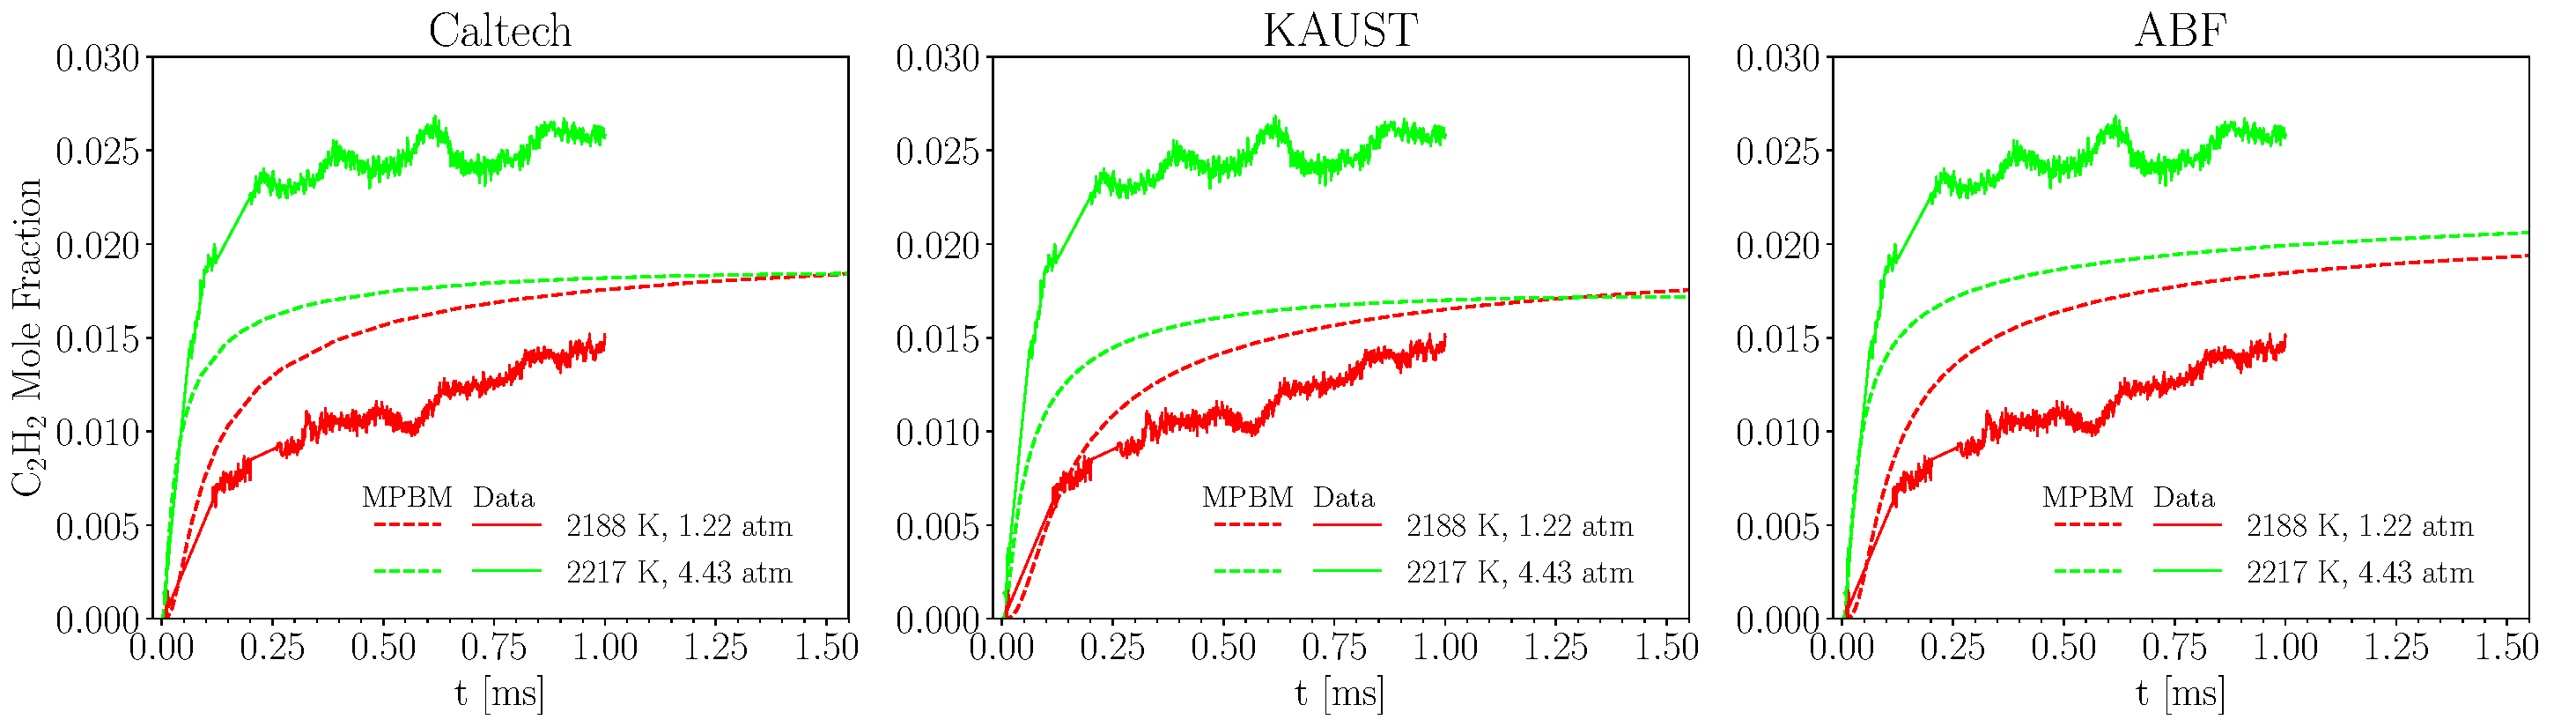
\includegraphics[width=0.9\textwidth]{Figures/Results/Shocktube/Stanford/September/stsh_sepmechs_C2H2.pdf}
	\caption{The time history of $\mathrm{C_2H_2}$ mole fraction during 10\% $\mathrm{CH_4}$ pyrolysis at T=2188 K, P=1.22 atm (red line) and T=2217 K, P=4.43 atm (green line) using Caltech, KAUST, and ABF mechanism with MPBM and Reactive Dimerization}
	\label{fig:shocktubes_sepc2h2} 
\end{figure}

\begin{figure}[H]
	\centering
	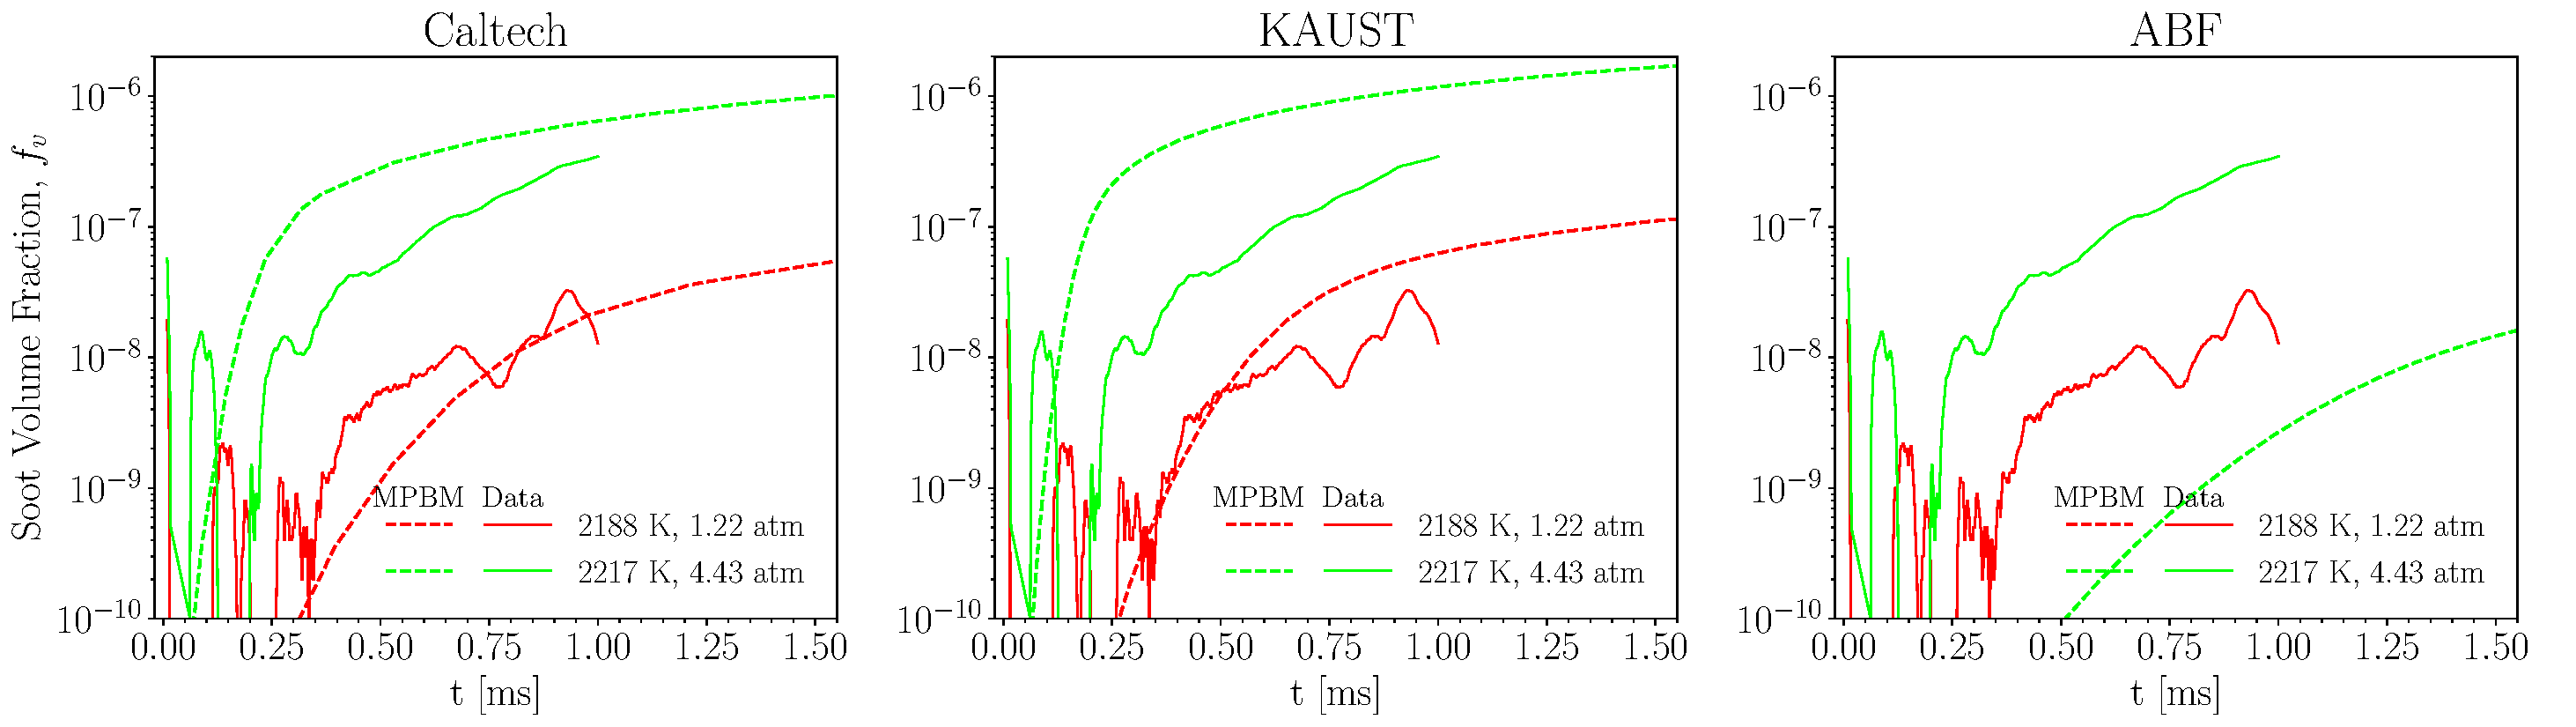
\includegraphics[width=0.9\textwidth]{Figures/Results/Shocktube/Stanford/September/stsh_sepmechs_vf.pdf}
	\caption{The time history of soot volume fraction, $f_v$ of 10\% $\mathrm{CH_4}$ pyrolysis at T=2188 K, P=1.22 atm (red line) and T=2217 K, P=4.43 atm (green line) using Caltech, KAUST, and ABF mechanism with MPBM and Reactive Dimerization}
	\label{fig:shocktubes_sepvf} 
\end{figure}

Fig.~\ref{fig:shocktubest_sepcasevf} shows the evolution of soot volume fraction, $f_v$ over simulation time in the temperature range (increasing from left to right) and (near) atmospheric and 4 atm pressure using KAUST mechanism. The upper and bottom rows correspond to 1 and 4 atm cases, and each column contains cases with similar temperatures. As expected, $f_v$ is not affected by particle dynamics model, but it increases with shock tube temperature. The time of $f_v=10^{-10}$ is shorter for 4 atm cases in each temperature indicating that pressure accelerates the soot formation. EF yields the most accurate $f_v$ prediction compared with the data in 2000-2500 K of 4 atm cases. The final $f_v$ predicted by increases by two orders of magnitude in 1900-2500 range at both pressures indicating more sensitivity of its inception rate to temperature.


\begin{figure}[H]
	\centering
	\includegraphics[width=1\textwidth]{Figures/Results/Shocktube/Stanford/September/stsh_cases_vf.pdf}
	\caption{The time history of soot volume fraction of 10\% $\mathrm{CH_4}$ pyrolysis in the temperature range of 1900-2500 K (increasing from left to right) and P=1$\pm$0.5 (bottom row) and 4$\pm$0.5 atm (upper row) using KAUST mechanism and different PAH growth and particle dynamics models}
	\label{fig:shocktubest_sepcasevf} 
\end{figure}

Figs.~\ref{fig:shocktubest_sepcasedp} and \ref{fig:shocktubest_sepcasedm} show time history of $d_p$ and $d_m$, respectively. The largest $d_p$ is predicted by RD in all cases with final values near 6 nm, which is close to $d_p$ of 10\% $\mathrm{CH_4}$. However, $d_m$ significantly decreased when feed-stock mole fraction is lowered from \%30 to \%10. Overall, the $d_p$ increases slightly with both temperature and pressure. RD has the largest $d_m$ in the entire temperature range of atmospheric cases, but at 4 atm $d_m$ by DC quickly increases and exceed RD due to stronger inception rate leading to larger coagulation rate and agglomerates. 

\begin{figure}[H]
	\centering
	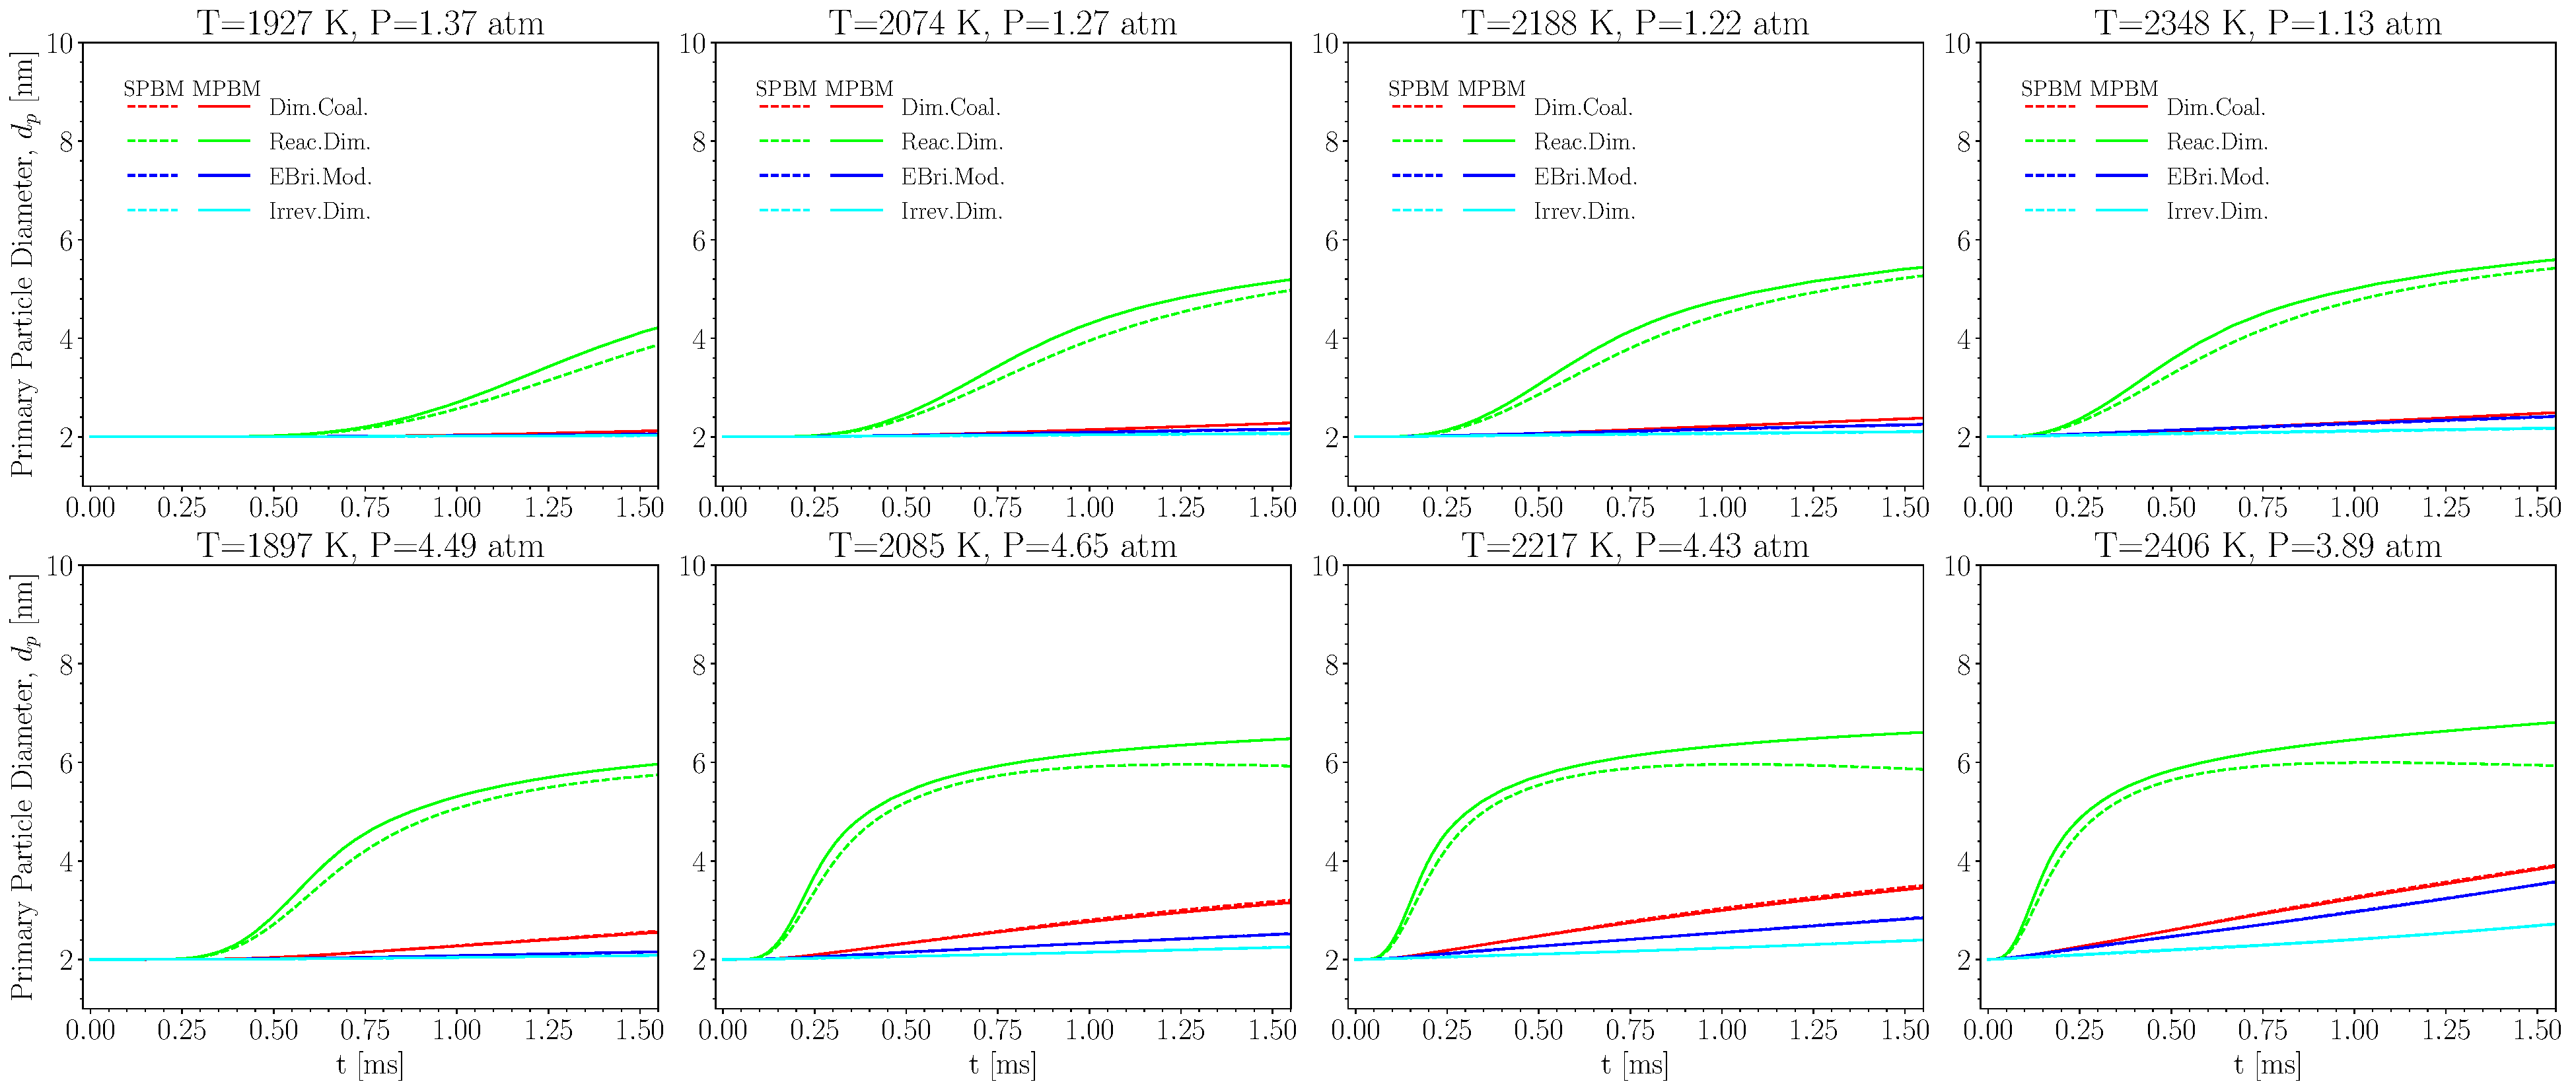
\includegraphics[width=1\textwidth]{Figures/Results/Shocktube/Stanford/june/stsh_cases_dp.pdf}
	\caption{The time history of primary particle diameter, $d_p$ of 30\% $\mathrm{CH_4}$ pyrolysis in the temperature range of 1800-2500 K and P=1$\pm$0.5 and 4$\pm$0.5 atm using KAUST mechanism and different PAH growth and particle dynamics models}
	\label{fig:shocktubest_sepcasedp} 
\end{figure}

\begin{figure}[H]
	\centering
	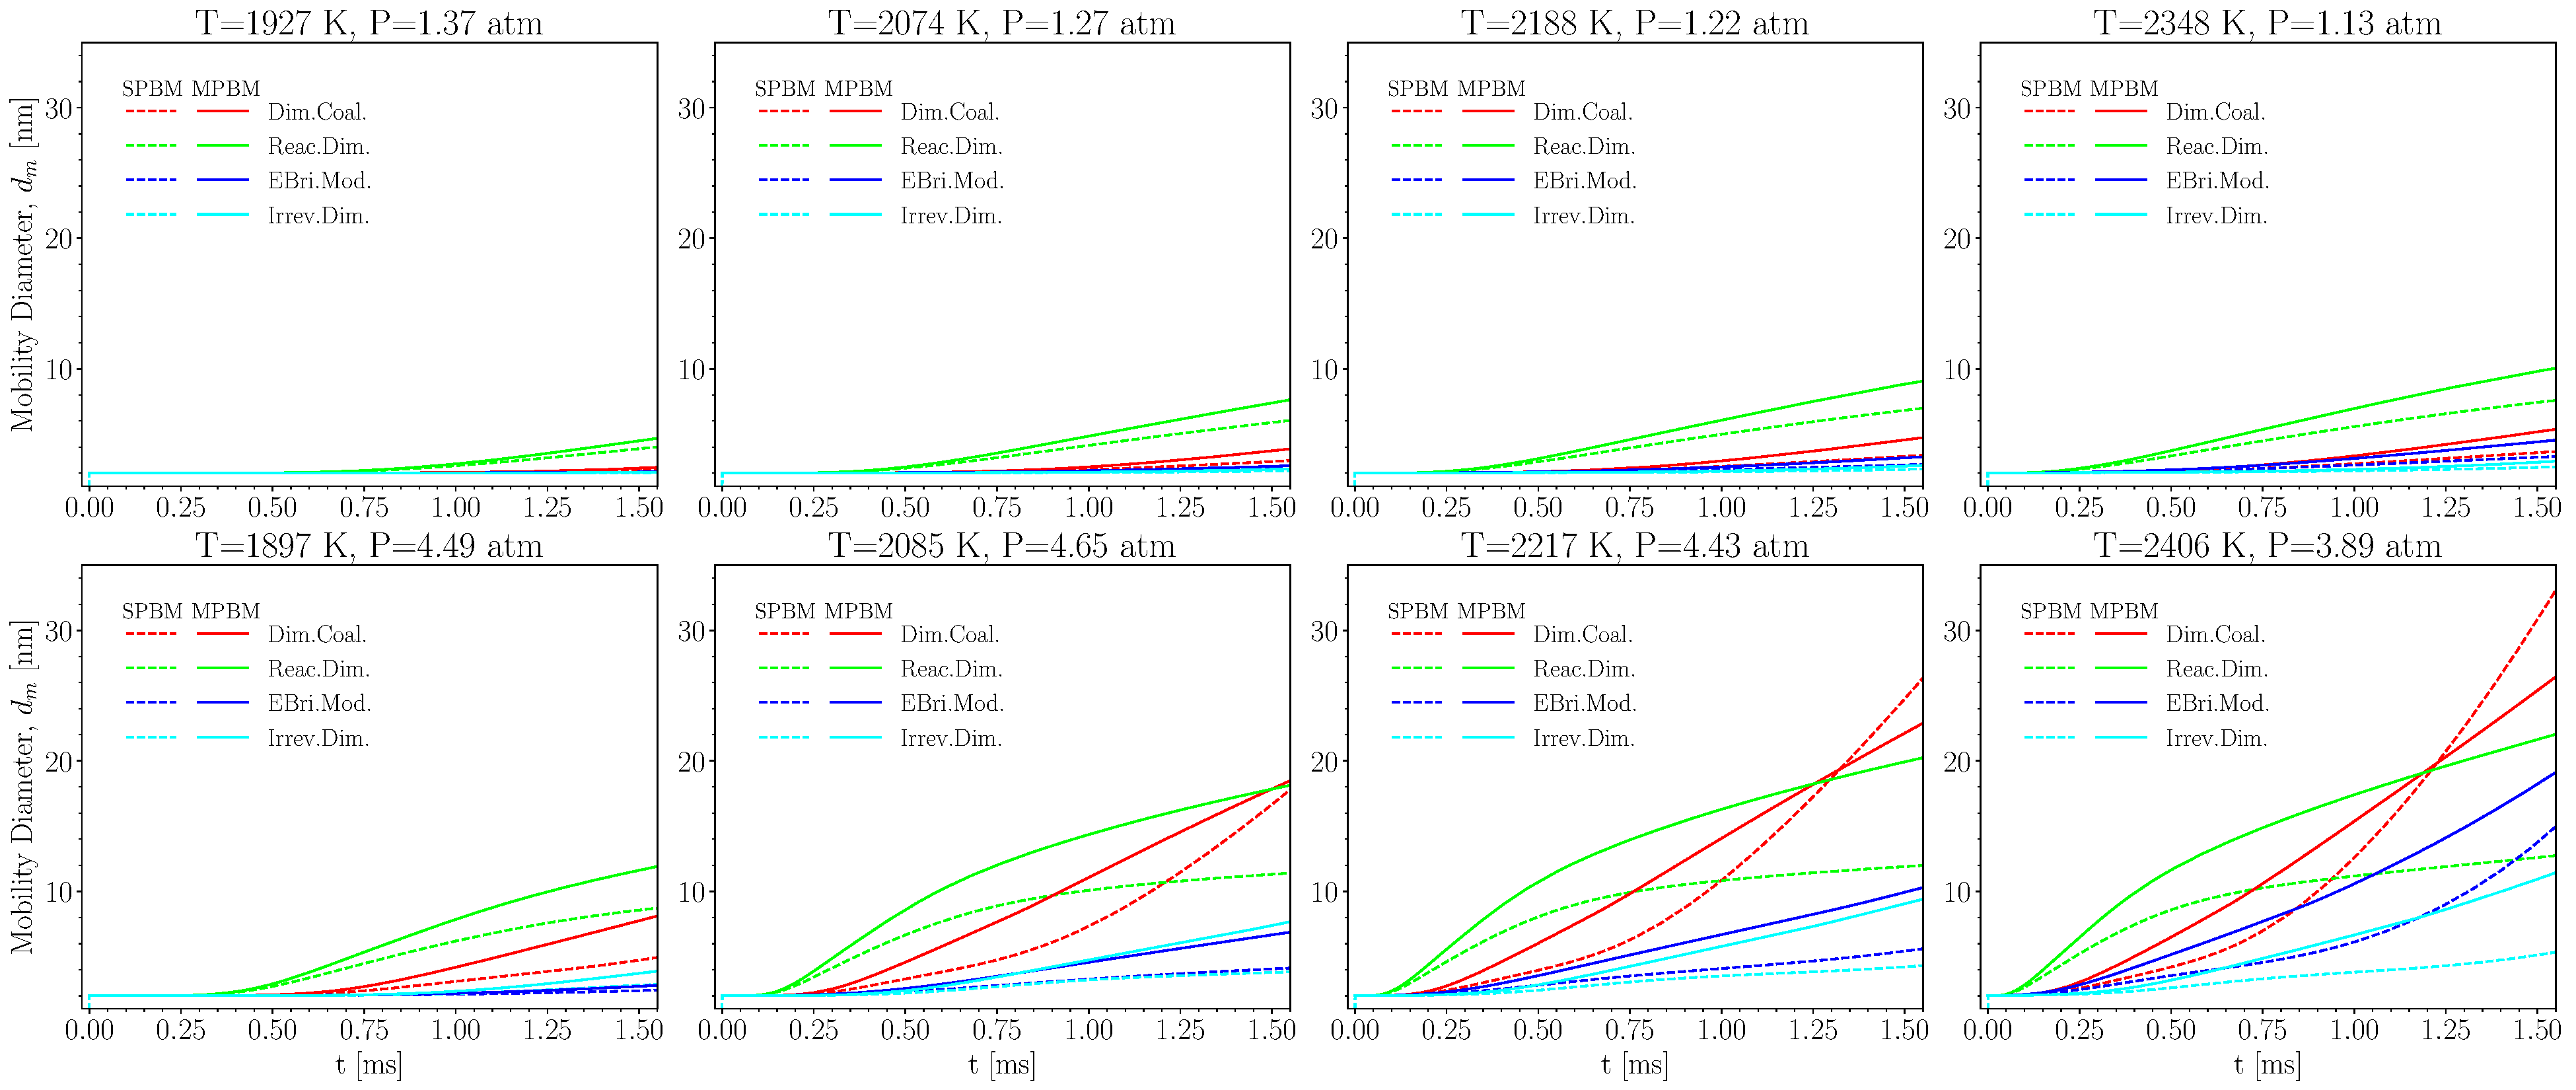
\includegraphics[width=1\textwidth]{Figures/Results/Shocktube/Stanford/September/stsh_cases_dm.pdf}
	\caption{The time history of mobility diameter, $d_m$ of 30\% $\mathrm{CH_4}$ pyrolysis in the temperature range of 1800-2500 K and P=1$\pm$0.5 and 4$\pm$0.5 atm using KAUST mechanism and different PAH growth and particle dynamics models}
	\label{fig:shocktubest_sepcasedm} 
\end{figure}

\subsection{Analysis of soot morphology in methane pyrolysis shock-tube}

The TEM images of 10\% $\mathrm{CH_4}$ at T=2230 K and P=4.5 atm data point provided by Stanford group are used to evaluate the performance of omnisoot in the prediction of $\mathrm{d_p}$ and $\mathrm{d_m}$ and compare the effect of different PAH growth and particle dynamics model on morphology. Soot particles are sampled from \hl{the end pipe wall} and analyzed using a \hl{****} Transmission Electron Microscopy model \hl{****} over \hl{****} TEM grid. As reported by Stanford team, the expansion wave traverses the shock tube around 2 ms reducing the temperature to nearly \hl{****} K freezing the chemical reactions that contribute to the surface growth, but the coagulation might continue until the collection of particles leading to larger agglomerates. As a result, $d_p$ estimated from the TEM images closely represents $d_p$ of agglomerates at the end of process, but TEM-based $d_m$ could be larger the actual values due to post expansion wave growth of particles. \textit{atems} package~\citep{sipkens2021using} was used for characterizing soot aggregates in TEM images with different methods for evaluating the aggregate projected area, perimeter, and primary particle diameter. It creates a binary map from the raw TEM image where white and black pixels represent the agglomerates and background, respectively, and feeds the map to a agglomerate segmentation algorithm to detect individual agglomerates. Fig.\ref{fig:shocktubest_binarymapprocess} shows a sample from TEM images and segmented agglomerates from generated map.

\begin{figure}[H]
	\centering
	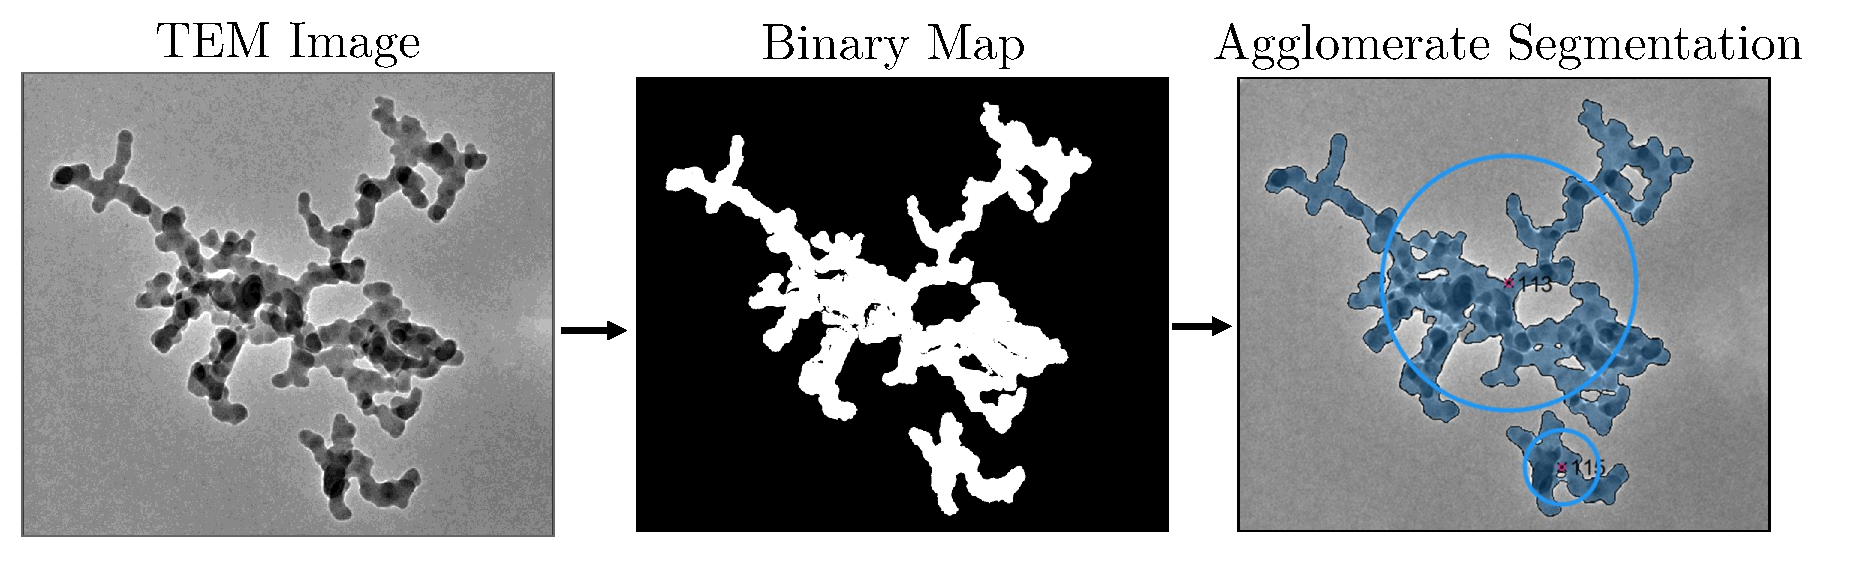
\includegraphics[width=0.9\textwidth]{Figures/Results/Shocktube/Stanford/TEM/binarymapprocess.pdf}
	\caption{A TEM image provided by Stanford group (left pane) with the generated binary map (middle pane) and detected agglomerates using the segmentation algorithm (right pane)}
	\label{fig:shocktubest_binarymapprocess} 
\end{figure}

We applied K-means clustering (KMC)~\citep{sipkens2021using} and otsu thresholding~\citep{dastanpour2016automated} to the same TEM images and compared the segmented agglomerates. A sample is shown in Fig.\ref{fig:shocktubest_aggseg_compare} where  KMC detected more agglomerates in the TEM image, but segments part of the background as agglomerates or divides a single agglomerate into multiple ones. On the other hand, otsu thresholding misses most of agglomerates in the TEM image. Here, the  K-means clustering~\citep{sipkens2021using} is used and 171 agglomerates were detected. $d_m$ was calculated from the diameter of equivalent projected area , $A_a$ of each agglomerate. The pair correlation method (PCM)~\citep{dastanpour2016automated} was applied to compute the projected primary particle area, $A_p$ and the mean $d_p$ assuming that primary particle are almost uniform in size within each agglomerate. The number of primary particle per agglomerate is calculated as $n_p=A_a/A_p$ resulting in 6554 primary particles. The mean $d_p$ of the entire samples is calculated as 

\begin{equation}
	\overline{d}_{p} = \frac{\sum_{Aggs} n_p d_p}{\sum_{Aggs} n_p} 
	\label{eqn:meandp}
\end{equation}


\begin{figure}[H]
	\centering
	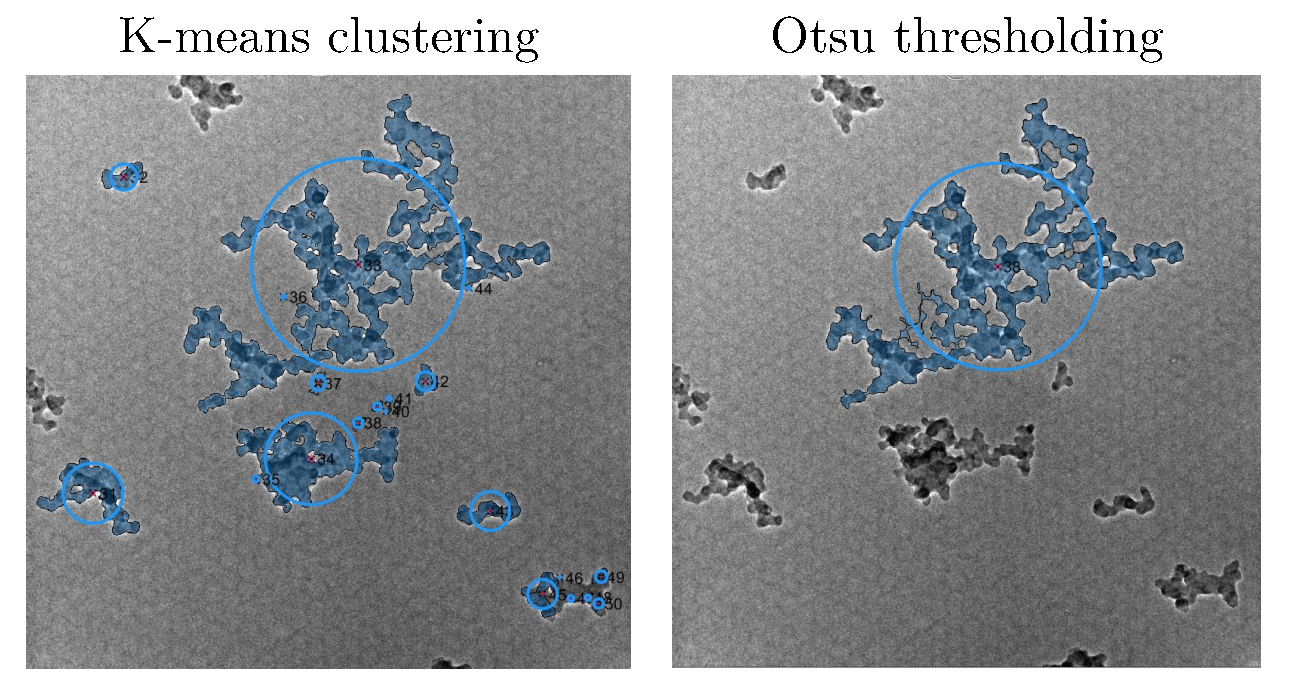
\includegraphics[width=0.6\textwidth]{Figures/Results/Shocktube/Stanford/TEM/aggseg_compare.pdf}
	\caption{Agglomerates in single TEM image segmented by K-means clustering (left pane) and otsu thresholding (right pane)}
	\label{fig:shocktubest_aggseg_compare} 
\end{figure}


\begin{table}
	\caption{The morphological characteristics of agglomerates quantified by atems using KMC and PCM}
	\label{tab:shocktube_TEM_morph}
	\centering
	\begin{tabular}{l l l}
		\hline
		Property & Arithmetic mean & Median \\
		\hline
		$d_m$ [nm] & 97 & 69 \\
		$d_p$ [nm] & 22 & 18 \\
		\hline
	\end{tabular}
\end{table}


Table~\ref{fig:shocktubest_aggseg_compare} reports the arithmetic mean and median of mobility and primary particle diameter detected by atems from TEM images. The computed $d_m$ and $d_p$ will be compared with soot sampled from various sources. Soot morphology is mainly governed by coagulation leading to self-similar structures in which $d_m$ scales with $d_p$ and $n_p$. Following that principle, a power-law derived from DEM simulation in flame conditions~\citep{Kelesidis2017} was introduced in Sec.~\ref{sec:sootmorphology}. Here, we compare the ratio of mobility to primary particle diameter $d_m/d_p$ with $d_m/d_p=n_p^{0.45}$ (Eq.~\ref{eqn:d_m}). \citet{olfert2019universal} analyzed soot particles from flares~\citep{kazemimanesh2019size}, inverted burners~\citep{dastanpour2017variation}, compression ignition engines~\citep{graves2015characterization} and other sources to support the external mixing hypothesis and related agglomerate size characterized by $d_m$ to $d_p$ using the following power-law:

\begin{equation}
	d_{p} = d_{p,100} 
	\left(
	\frac{d_m}{100 nm}
	\right)^{D_{\mathrm{TEM}}},
	\label{eqn:usf}
\end{equation}

\noindent where $d_{p,100}$ is the average primary particle diameter for a 100 nm aggregate, and $D_{\mathrm{TEM}}$ is the exponent. Both quantities were obtained by fitting Eq.~\eqref{eqn:usf} to soot sampled from different sources. the left pane of Fig~\ref{fig:shocktube_TEM_powerlaws} demonstrates the ratio of mobility to primary particle diameter, $d_m/d_p$ from TEM images analyzed by atems compared with the DEM derived power-law (Eq.~\eqref{eqn:d_m}). In the right pane of the same Figure, the scatter plot of $d_p$ against $d_m$ is compared with power-law curves of Eq.~\eqref{eqn:usf} using two sets of prefactor and exponent values, i) $D_{\mathrm{TEM}}$=0.32, $d_{\mathrm{p,100}}$=20.6 nm, and ii) $D_{\mathrm{TEM}}$=0.39, $d_{\mathrm{p,100}}$=20.2 nm taken from average values reported in summary of fit parameters in Table 1 of \citet{olfert2019universal}. Both power-laws show a good agreement with quantities obtained from TEM images with DEM power-law reaching the maximum different of 35\% indicating that $d_p$ and $d_m$ computed by atems can be good representative of soot agglomerates with minimal agglomerate overlap.

\begin{figure}[H]
	\centering
	\begin{subfigure}[t]{0.32\textwidth}
		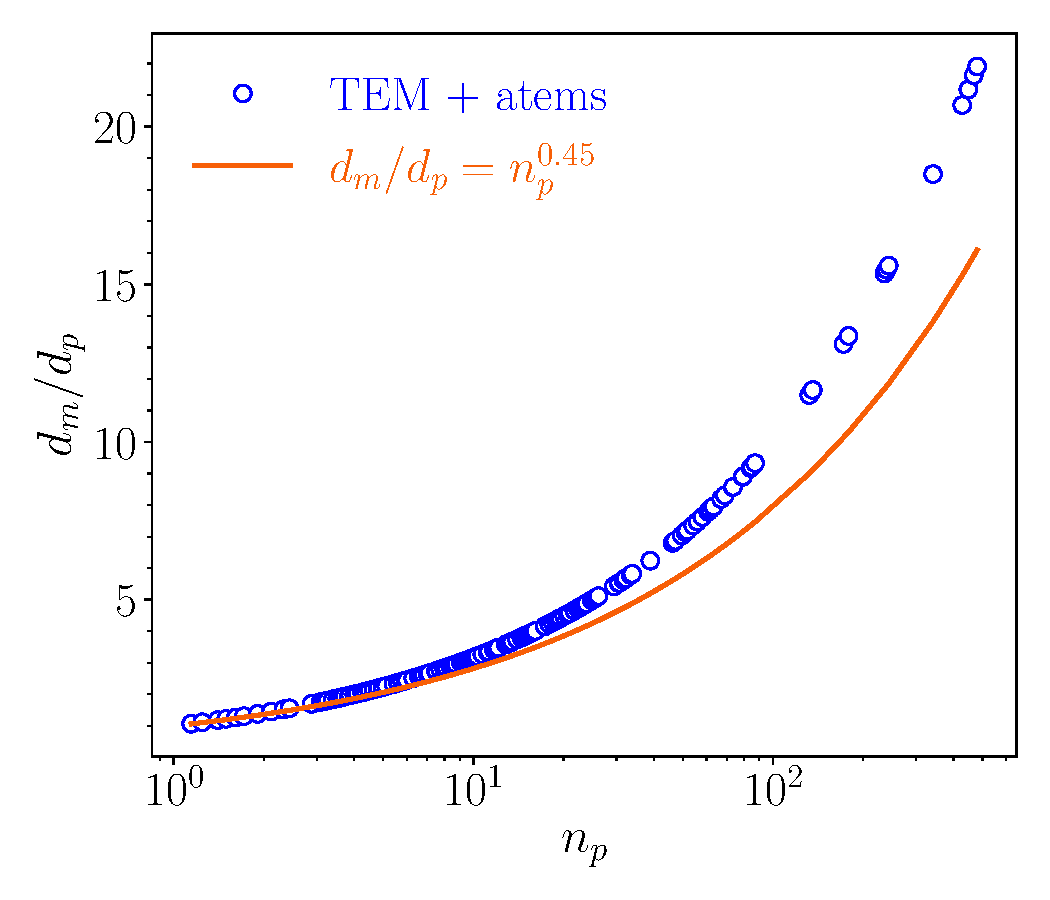
\includegraphics[width=1\textwidth]{Figures/Results/Shocktube/Stanford/TEM/dm_scalelaw.pdf}
	\end{subfigure}
	\begin{subfigure}[t]{0.32\textwidth}
		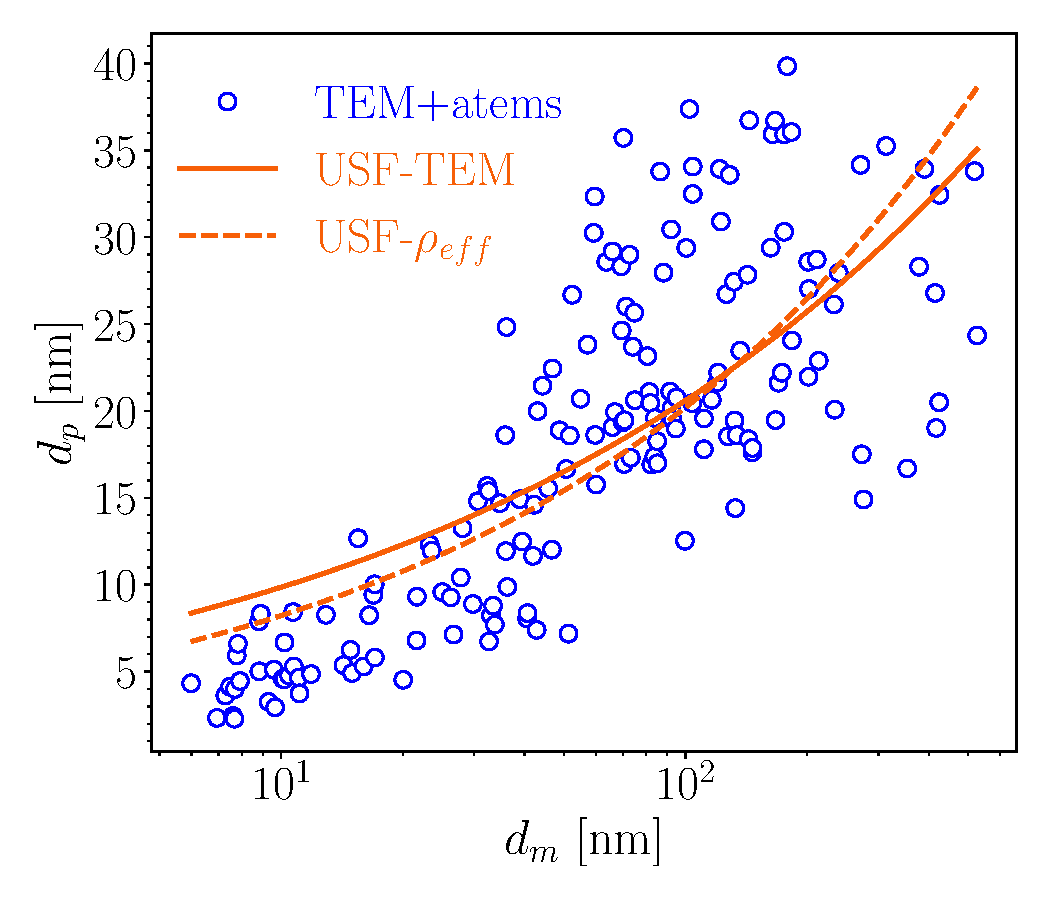
\includegraphics[width=1\textwidth]{Figures/Results/Shocktube/Stanford/TEM/dmdp_scalelaw.pdf}
	\end{subfigure}
	\caption{The ratio of mobility to primary particle diameter $d_m/d_p$ from TEM image obtained by atems~\citep{sipkens2021using} (symbols) compared with the DEM derived power law $d_m/d_p=n_p^{0.45}$~\citep{Kelesidis2017} (left pane) and the $d_m$ as a function of $d_p$ compared with power law in Eq.~\eqref{eqn:usf} (right pane)} 
	\label{fig:shocktube_TEM_powerlaws} 
\end{figure}

Fig.~\ref{fig:shocktube_TEM_fvdd} compares $f_v$ from extinction measurement, $d_p$ and $d_m$ computed from TEM images with model predictions using KAUST mechanism, Monodisperse and different PAH growth models. The horizontal error bars denotes the uncertainty in residence time that TEM measurements correspond to. As reported by Stanford group, the expansion wave propagates near t=2 ms stopping the growth of $d_p$. Although the predicted soot mass, represented by volume fraction, is close even greater than measurements, but $d_p$ is underpredicted by all PAH growth models. RD yields the largest $d_p$ near 7 nm that is lower than $d_p$ from TEM measurements by a factor of 3.

\begin{figure}[H]
	\centering
	\begin{subfigure}[t]{0.3\textwidth}
		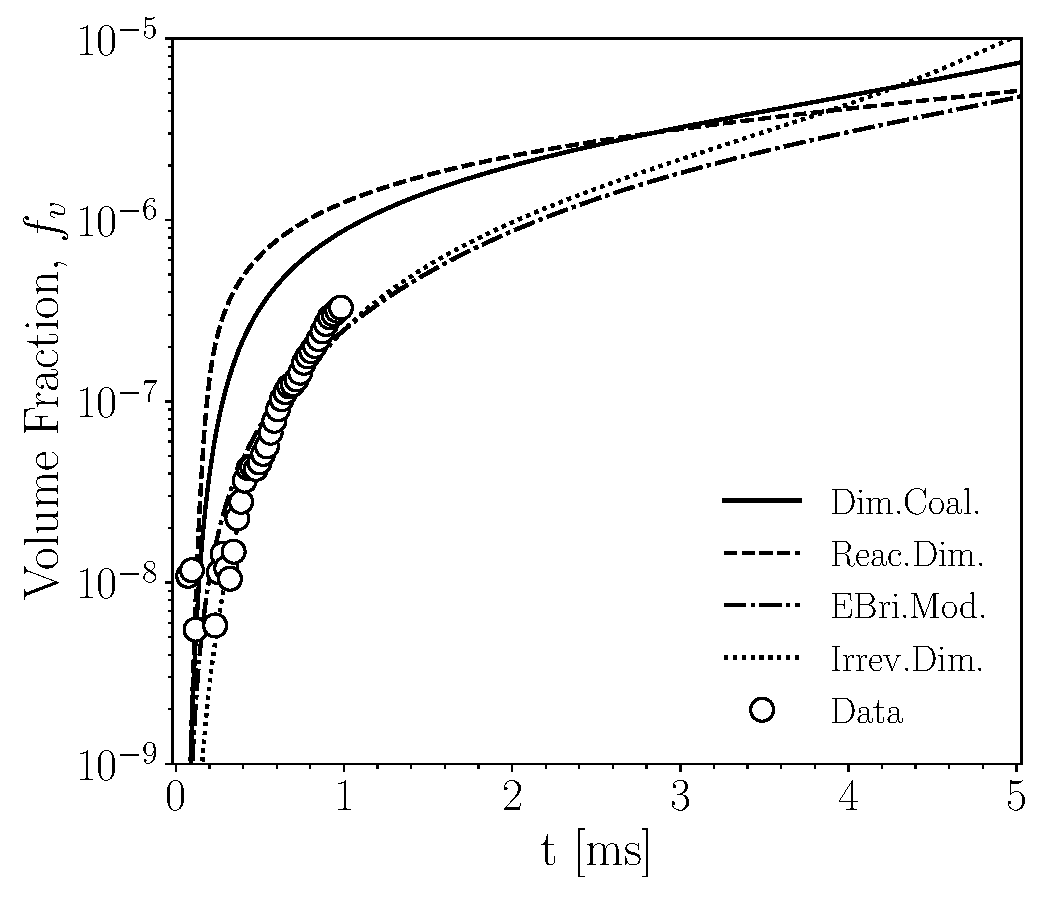
\includegraphics[width=1\textwidth]{Figures/Results/Shocktube/Stanford/TEM/vf_TEM.pdf}
	\end{subfigure}
	\begin{subfigure}[t]{0.32\textwidth}
		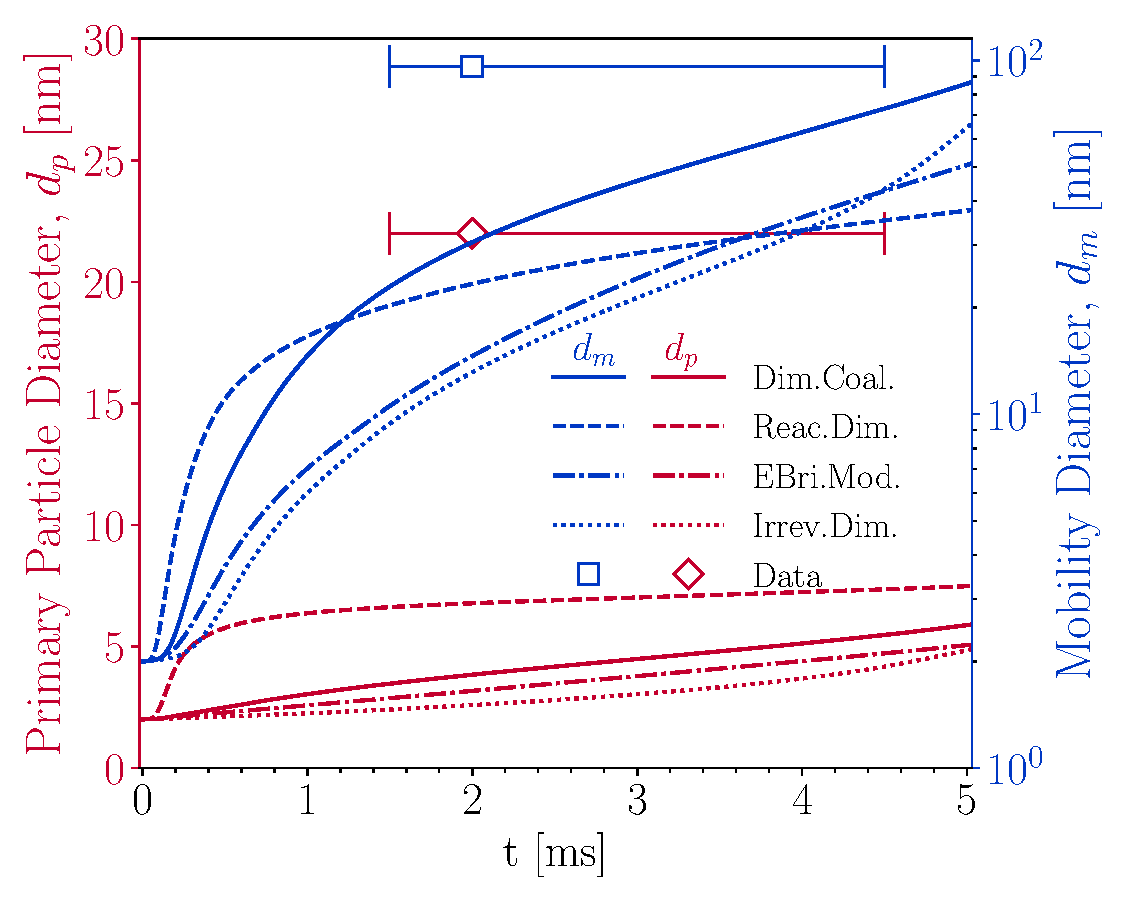
\includegraphics[width=1\textwidth]{Figures/Results/Shocktube/Stanford/TEM/dp_dm_TEM.pdf}
	\end{subfigure}
	\caption{The volume fraction, $f_v$ (left pane) and mobility, $d_m$ (blue lines in right pane) and primary particle diameter, $d_p$ (red lines in right pane) predicted by KAUST mechanism, MPBM, and different PAH growth models at T=2230 K, P=4.5 atm that corresponds to shock-tube conditions of TEM measurement}
	\label{fig:shocktube_TEM_fvdd} 
\end{figure}

\subsection{Sensitivity of yield and morphology to inception and surface growth rate}

The underprediction of $d_p$ by the model despite producing enough or even more soot carbon mass compared with the measurement motivated performing a sensitivity analysis for soot yield and morphology, especially because of uncertainties in inception and surface growth pathways and reaction rates associated with the PAH growth models integrated in omnisoot. It should be noted that this section is not aimed at a systematic sensitivity analysis with respect to all reaction rates, but rather to determine which sub-model has the dominant effect on yield and morphology that can be modified within the physical constraints to tailor these quantities to the desired values.

First, we examine the effect of HACA rates on yield and morphology of soot generated during 10\% $\mathrm{CH_4}$ at T=2230 K and P=4.5 atm in the Stanford shock-tube. To this  purpose, the surface reactivity, $\alpha$, in HACA formulation is modified by introducing a damping factor, $\zeta$ in Eq.~\eqref{eqn:hacaRate} as:

\begin{equation}
	\alpha^i = \tanh 
	\left(
	\frac{12.56 - 0.00563\cdot \zeta T}
	{\mbox{log}_{10}
		\left( \frac{\rho_{soot}\cdot Av}{W_{carbon}} \frac{\pi}{6}{d^i_p}^3 \right) } -1.38+0.00068\cdot \zeta T
	\right)
	\label{eqn:alpha_modified}.
\end{equation}

Note that, there are many adjustable parameters in HACA scheme such as rate constants. $\zeta$ to modify $\alpha$ is intentionally chosen for a number of reasons. First, $\alpha$ was initially introduced as a tuning parameter as a function of local temperature and primary particle diameter to control surface growth rate, and it has been usually adjusted specifically for each flame~\citep{castaldi1996pah, xu1997soot} to match the predicted volume fraction with the measurements. Second, the global empirical relation of \citet{appel2000kinetic} (used omnisoot to quantify $\alpha$) developed by fitting parameters of $\alpha$ to minimize the prediction error of volume fraction for various premixed flames, and shock tubes generally have larger temperature ranges compared with premixed flames, which could excessively reduce surface reactivity and HACA growth rates. Finally, larger volume fractions (in the order of few ppm) were underpredicted by the global $\alpha$ relation (Fig. 9 of \citep{appel2000kinetic}). So, the low values of $\alpha$ in the shock tube at T=2230 K corresponding to process conditions of TEM measurements can contribute to underprediction of surface growth rates and $d_p$. We introduce $\zeta$ to reduce the damping effect of temperature on surface reactivity. Fig.~\ref{fig:shocktube_alpha_HACA} demonstrates the variation of $\alpha$ with temperature for $\zeta$=0.6, 0.8, 1 and primary particle diameter 2 and 6 nm. $\alpha$ decreases with temperature, and it is inversely proportional to $\zeta$. 

\begin{figure}[H]
	\centering
	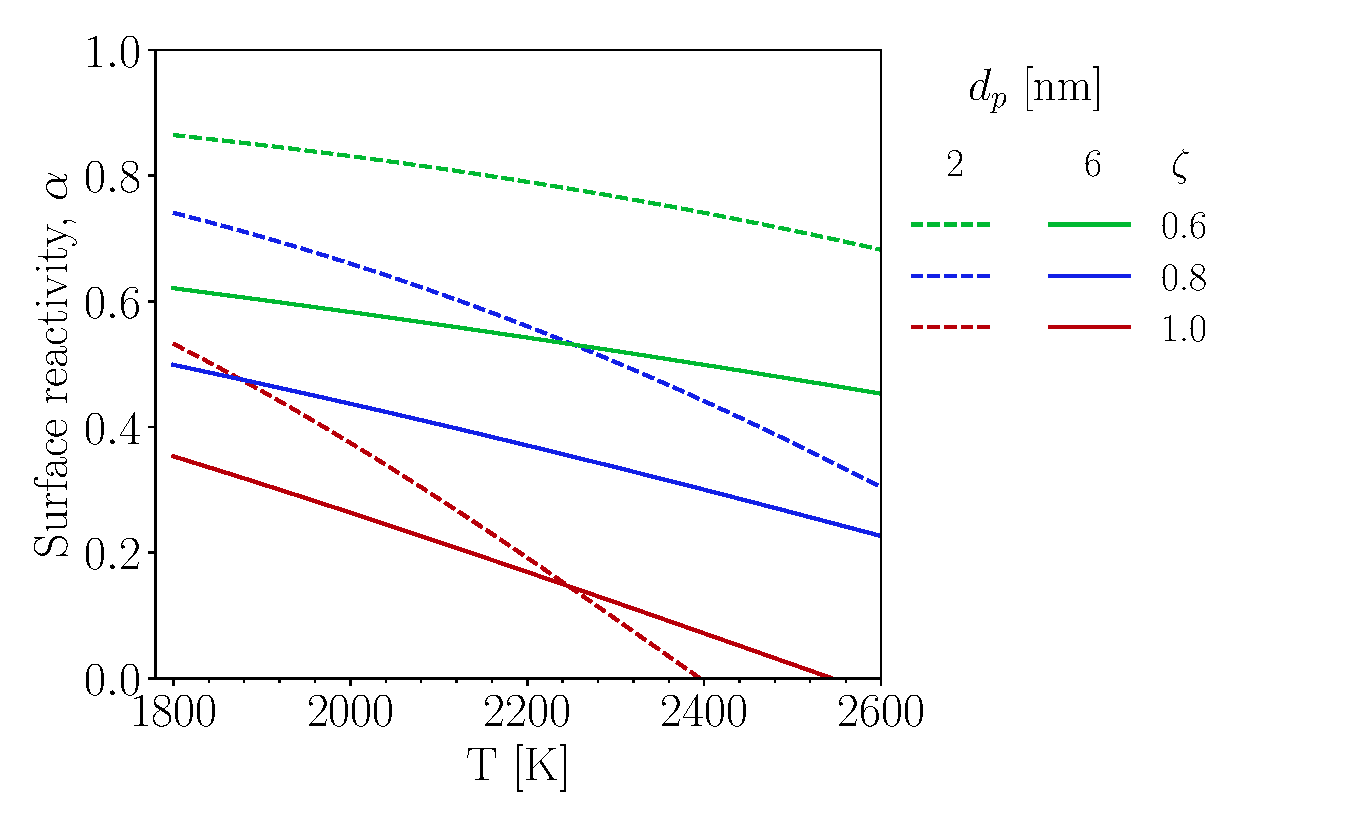
\includegraphics[width=0.5\textwidth]{Figures/Results/Shocktube/HACA/alpha.pdf}
	\caption{The variation of surface reactivity, $\alpha$, as a function of temperature for different values of $\zeta$ and primary particle size of 2 nm (dashed lines) and 6 nm (solid lines)}
	\label{fig:shocktube_alpha_HACA} 
\end{figure}

A series of simulation were performed to study the damping effect of temperature on soot mass and morphology by varying   $\zeta$ from 1 to 0.8 and 0.6. Note that, $\zeta$ of 1 represent the original $\alpha$ formulation. The reaction mechanism and particle dynamic model were set to KAUST and MPBM, respectively, but all PAH growth were used in the simulations.
Fig.~\ref{fig:shocktube_vf_zetseffect} and~\ref{fig:shocktube_sy_zetseffect} depicts the volume fraction and soot carbon yield, respectively. As expected, both quantities increases by reducing $\zeta$. The difference due to three $zeta$ values become significant only after t=1.5 ms, so it does not change the agreement with measurements available up to 1 ms. The final SY at the end of 5 ms increases by a factor of 1.3 to 2 depending on the PAH growth model by varying $\zeta$ from 1 to 0.6. Additionally, soot yield for DC, EF, and ID models levels off towards the end of simulation indicting the maximum yield.

\begin{figure}[H]
	\centering
	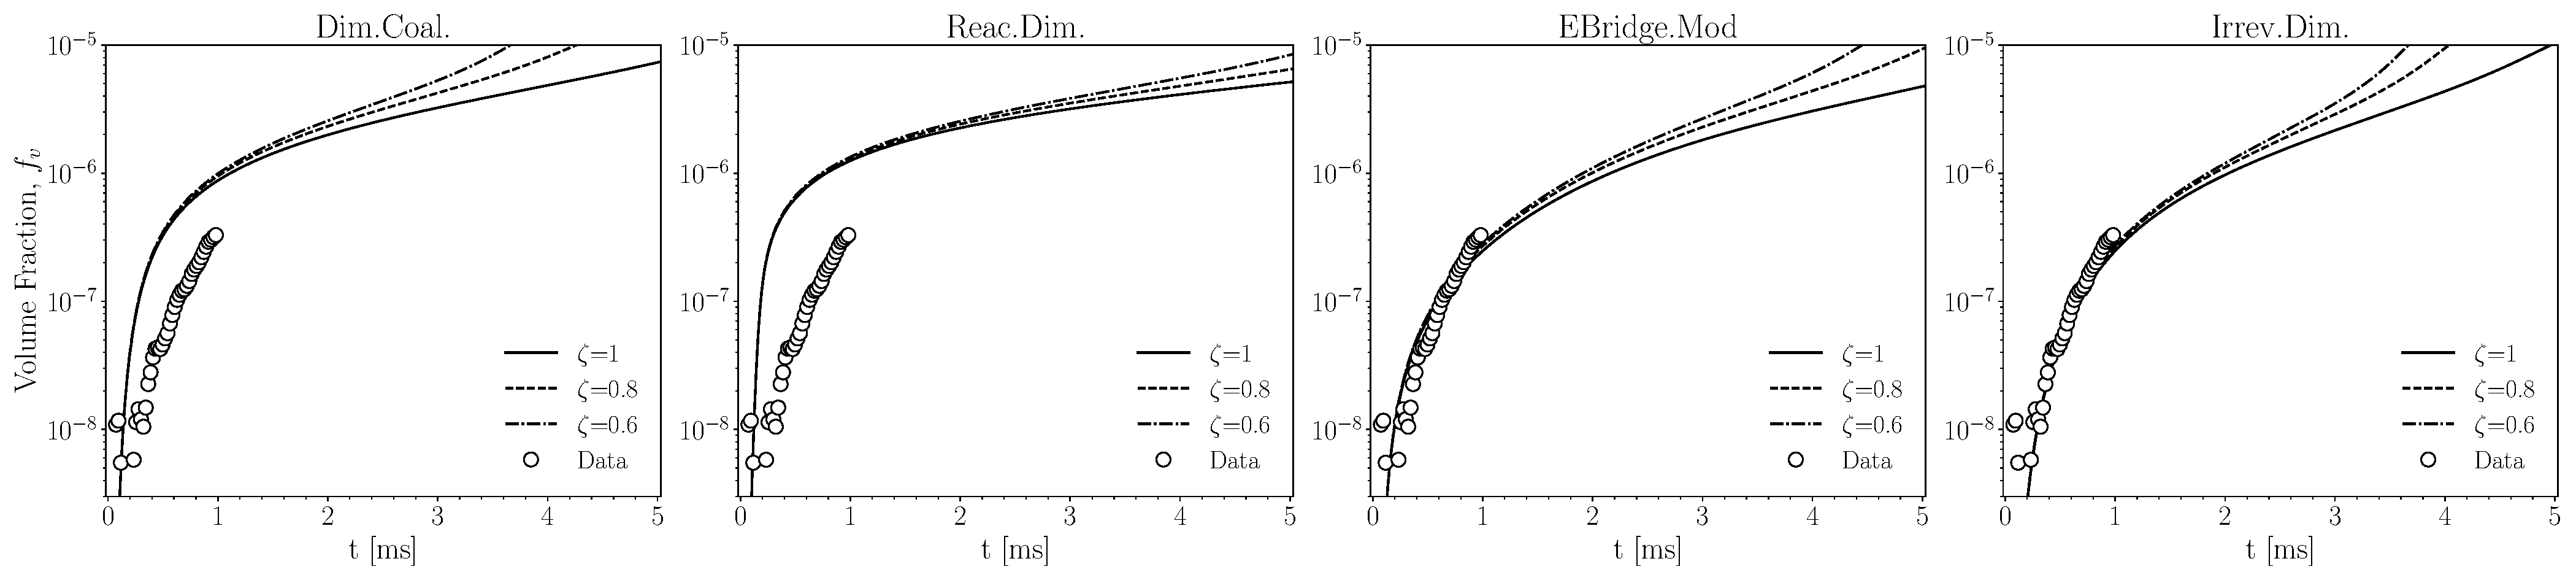
\includegraphics[width=1\textwidth]{Figures/Results/Shocktube/Stanford/TEM/vf_all_zetaeffect.pdf}
	\caption{The effect of reducing $\zeta$ leading to larger HACA rates on soot volume fraction, $f_v$ using KAUST and MPBM and different PAH growth model}
	\label{fig:shocktube_vf_zetseffect} 
\end{figure}


\begin{figure}[H]
	\centering
	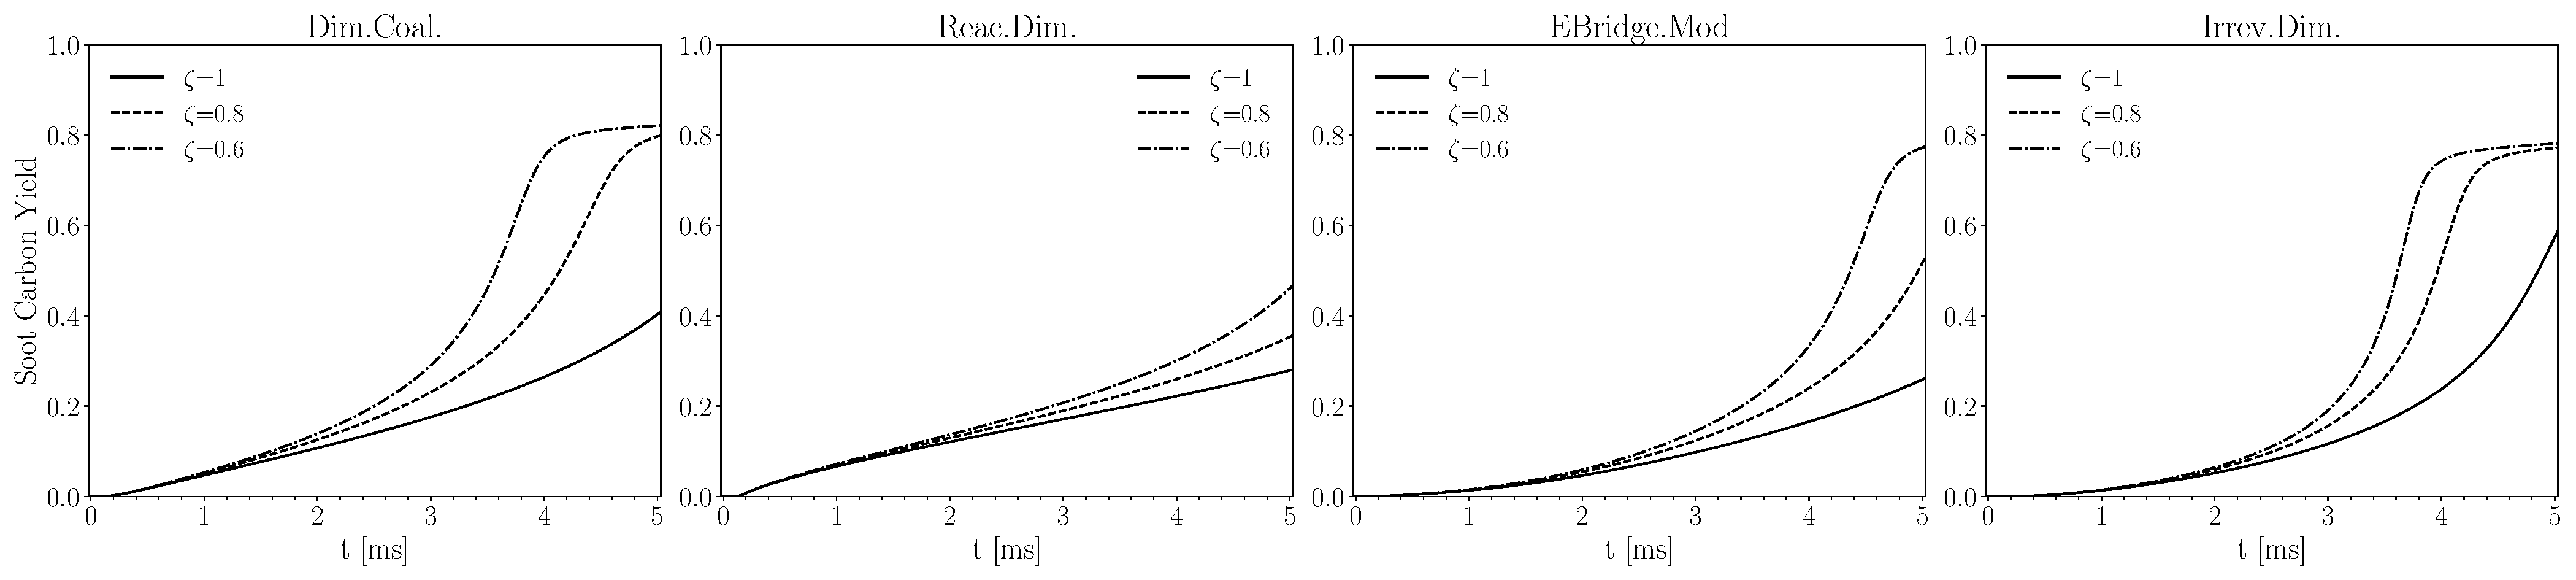
\includegraphics[width=1\textwidth]{Figures/Results/Shocktube/Stanford/TEM/sy_all_zetaeffect.pdf}
	\caption{The effect of reducing $\zeta$ leading to larger HACA rates on soot carbon yield using KAUST and MPBM and different PAH growth model}
	\label{fig:shocktube_sy_zetseffect} 
\end{figure}

Fig.\ref{fig:shocktube_ddd_zetseffect} demonstrates changes of $d_p$ and $d_m$ due to $\zeta$ values using different PAH growth models. Reducing $\zeta$ to 0.6 increases $d_p$ to a maximum of 2 nm. $d_p$ predicted by DC, EF, and ID model reaches its maximum indicating that smaller $\zeta$ values (higher HACA rate) will not change the maximum $d_p$. The simulations using different $\zeta$ values highlight relatively low sensitivity of $d_p$ with respect to surface reactivity in 10\% $\mathrm{CH_4}$ pyrolysis in shock tube described using a constant volume reactor.

\begin{figure}[H]
	\centering
	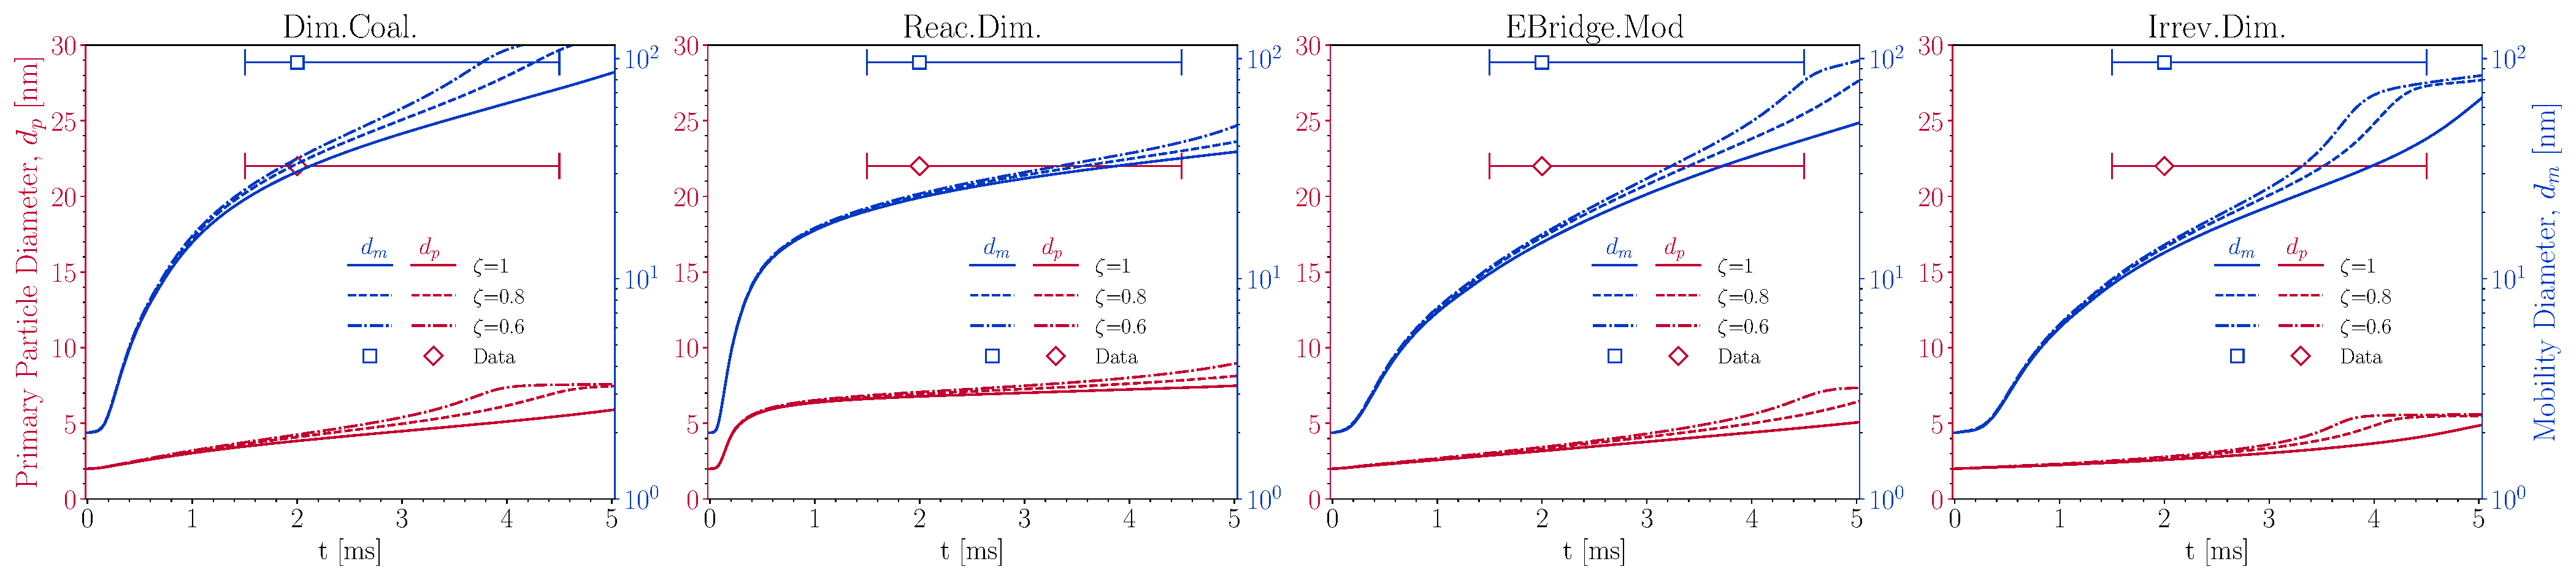
\includegraphics[width=1\textwidth]{Figures/Results/Shocktube/Stanford/TEM/dp_dm_zetaeffect.pdf}
	\caption{The effect of reducing $\zeta$ leading to larger HACA rates on mobility, $d_m$ and primary particle diameter, $d_p$ using KAUST and MPBM and different PAH growth model}
	\label{fig:shocktube_ddd_zetseffect} 
\end{figure}